\documentclass[mathserif,11pt]{beamer}
%%%%%%%%%%%%%%%%%%%%%%%%%%%%%%%%%%%%%%%%%%%%%%%%%%%%%%%%%%%%%%%%%%%%%%%%%%%%%%%%%%%%%%%%%%%%%%%%%%%%%%%%%%%%%%%%%%%
% Appearance
\mode<presentation>
{
	\usetheme{CambridgeUS}
	\usecolortheme{whale}
	\setbeamercovered{transparent}
}
% Redefine beamer colors
\definecolor{UoNblue1}{RGB}{0,155,189}
\definecolor{UoNblue2}{RGB}{0,125,168}
\definecolor{UoNblue3}{RGB}{0,86,151}
\definecolor{UoNblue4}{RGB}{27,42,107}
\definecolor{UoNblue5}{RGB}{25,26,79}
% Captions and titles
\setbeamertemplate{caption}{\raggedright\insertcaption} 
\setbeamercolor{frametitle}{fg=UoNblue3}
\setbeamercolor{title}{bg=UoNblue2}

\setbeamercolor{palette primary}{fg=white, bg=UoNblue3}
\setbeamercolor{palette secondary}{fg=white, bg=UoNblue4}
\setbeamercolor{palette tertiary}{fg=white, bg=UoNblue5}
% Outline slide
\setbeamertemplate{section in toc}[circle]
\setbeamerfont{section number projected}{family=\rmfamily,series=\bfseries,size=\normalsize}
\setbeamercolor{section number projected}{bg=UoNblue5,fg=white}
% Itemize list
\setbeamertemplate{itemize item}[circle]
\setbeamertemplate{itemize subitem}[circle]
\setbeamercolor{itemize item}{fg=UoNblue4}
\setbeamercolor{itemize subitemitem}{fg=UoNblue5}
% Title box
\setbeamertemplate{frametitle}{%
	\nointerlineskip%
	\begin{beamercolorbox}[wd=\paperwidth,ht=2.0ex,dp=0.6ex]{frametitle}
		\hspace*{1ex}\insertframetitle%
	\end{beamercolorbox}%
}
%%%%%%%%%%%%%%%%%%%%%%%%%%%%%%%%%%%%%%%%%%%%%%%%%%%%%%%%%%%%%%%%%%%%%%%%%%%%%%%%%%%%%%%%%%%%%%%%%%%%%%%%%%%%%%%%%%%
\usepackage[english]{babel}
% or whatever
\usepackage[latin1]{inputenc}
% or whatever
\usepackage{array} % To vertically center tabular content 
\usepackage{times}
\usepackage[T1]{fontenc}
%\usepackage{eulervm}
%\usepackage{cmbright}
%%%%%%%%%%%%%%%%%%%%%%%%%%%%%%%%%%%%%%%%%%%%%%%%%%%%%%%%%%%%%%%%%%%%%%%%%%%%%%%%%%%%%%%%%%%%%%%%%%%%%%%%%%%%%%%%%%%%
%\usepackage{tikz}
\usepackage{pgfplots}
\usepackage{tikz-3dplot}
\tdplotsetmaincoords{60}{-30}
\tdplotsetrotatedcoords{0}{90}{90}
\pgfplotsset{every axis/.append style={line width=0.5pt},label style={font=\scriptsize},tick label style={font=\scriptsize},x tick label style={/pgf/number format/.cd,fixed,precision=3, set thousands separator={}},z tick label style={/pgf/number format/.cd,fixed,precision=3, set thousands separator={}}}
\usetikzlibrary{shapes,shadows,arrows,backgrounds,patterns,positioning,automata,calc,decorations.markings,decorations.pathreplacing,bayesnet,arrows.meta}
\usepackage{amsmath,amssymb,mathrsfs,amsfonts,amsthm} % for maths
\usepackage{graphicx}
\usepackage{animate}
%\usepackage{subfig}
\usepackage{eucal}    % for curly math letter symbols
\usepackage{amssymb}  % for ams symbols
\usepackage{pifont}
\usepackage{color} %Invoke options usenames,dvipsnames for larger color choice
\usepackage{microtype} % Slightly tweak font spacing for aesthetics
\usepackage{multicol} % Used for the two-column layout of the document
%%%%%%%%%%%%%%%%%%%%%%%%%%%%%%%%%%%%%%%%%%%%%%%%%%%%%%%%%%%%%%%%%%%%%%%%%%%%%%%%%%%%%%%%%%%%%%%%%%%%%%%%%%%%%%%%%%%%
\DeclareSymbolFontAlphabet{\mathcal} {symbols}
\DeclareSymbolFont{symbols}{OMS}{cm}{m}{n}
\DeclareMathAlphabet{\mathbfit}{OML}{cmm}{b}{it}
\newcommand\id{\ensuremath{\mathbbm{1}}} 
\DeclareMathOperator{\E}{\mathbb{E}}
\DeclareMathOperator{\eye}{\mathbb{I}}
\DeclareMathOperator{\zeros}{\mathbb{O}}
\DeclareMathOperator{\tr}{\textrm{tr}}
\DeclareMathOperator{\vc}{\textrm{vec}}
\DeclareMathOperator{\rk}{\textrm{rk}}
\DeclareMathOperator{\ik}{\mathrm{k}}
\DeclareMathOperator{\ip}{\mathrm{p}}
\DeclareMathOperator{\inn}{\mathrm{n}}
\DeclareMathOperator{\im}{\mathrm{m}}
\DeclareMathOperator{\td}{\mathrm{t}}
\DeclareMathOperator{\kd}{\mathrm{k}}
\DeclareMathOperator{\T}{\mathrm{T}}
\DeclareMathOperator{\K}{\mathrm{K}}
%%%%%%%%%%%%%%%%%%%%%%%%%%%%%%%%%%%%%%%%%%%%%%%%%%%%%%%%%%%%%%%%%%%%%%%%%%%%%%%%%%%%%%%%%%%%%%%%%%%%%%%%%%%%%%%%%%%%
\usepackage[backend=bibtex,style=ieee]{biblatex} % bibliography
\bibliography{bibliography}
\renewcommand*{\bibfont}{\footnotesize}
%%%%%%%%%%%%%%%%%%%%%%%%%%%%%%%%%%%%%%%%%%%%%%%%%%%%%%%%%%%%%%%%%%%%%%%%%%%%%%%%%%%%%%%%%%%%%%%%%%%%%%%%%%%%%%%%%%%%
% Populate title page
\title[AMR in poultry litter] % (optional, use only with long paper titles)
{Antimicrobial resistance in chicken manure heaps: UK composting experiment}
\author[A. Kadochnikova]{A. Kadochnikova\inst{1}}
\institute[UoN]{\inst{1}
	School of Mathematical Sciences\\
	The University of Nottingham}
\date{18 March 2024}
\logo{
\begin{tikzpicture}[overlay,remember picture]
\node[right=0.05cm] at (current page.212){
\includegraphics[height=0.7cm]{UoNlogoFC}};
\end{tikzpicture}}
\begin{document}
\begin{frame}
	\titlepage
\end{frame}
\begin{frame}{Outline}
\tableofcontents[hideallsubsections]
\end{frame}
%\subsection{Prototype in action}
%\begin{frame}{3D simulation of a self-heating compost heap}
%	\centering
%\animategraphics[loop,width=11cm]{10}{Figures/sh}{1}{122}	
%\end{frame}
%%%%%%%%%%%%%%%%%%%%%%%%%%%%%%%%%%%%%%%%%%%%%%%%%%%%%%%%%%%%%%%%%%%%%%%%%%%%%%%%%%%%%%%%
\section{Prototype informs experiment design}
%%%%%%%%%%%%%%%%%%%%%%%%%%%%%%%%%%%%%%%%%%%%%%%%%%%%%%%%%%%%%%%%%%%%%%%%%%%%%%%%%%%%%%%%
\begin{frame}{Prototyping output}
	\begin{itemize}
		\item Rapid heating followed by steadily high temperature, then slow cooling: must adjust frequency of biota sampling to capture interactions with temperature
		\item Sharp temperature gradients within heap: must sample across the heap, not just core and 
		\item Convective flux cools the heap faster than radiative flux: avoid direct contact with the soil
		\item Simple geometry is best: use wooden pellets
		\item pH does not have strong effect: sample to see what levels it reaches
		\item water activity is essential: measure moisture content and know litter composition
	\end{itemize}
\end{frame}
\begin{frame}{Composting experiment}
6 replicates observed for 75 days starting 09/01/2022:\\
	\begin{columns}
	\begin{column}{0.5\textwidth}
		\centering
		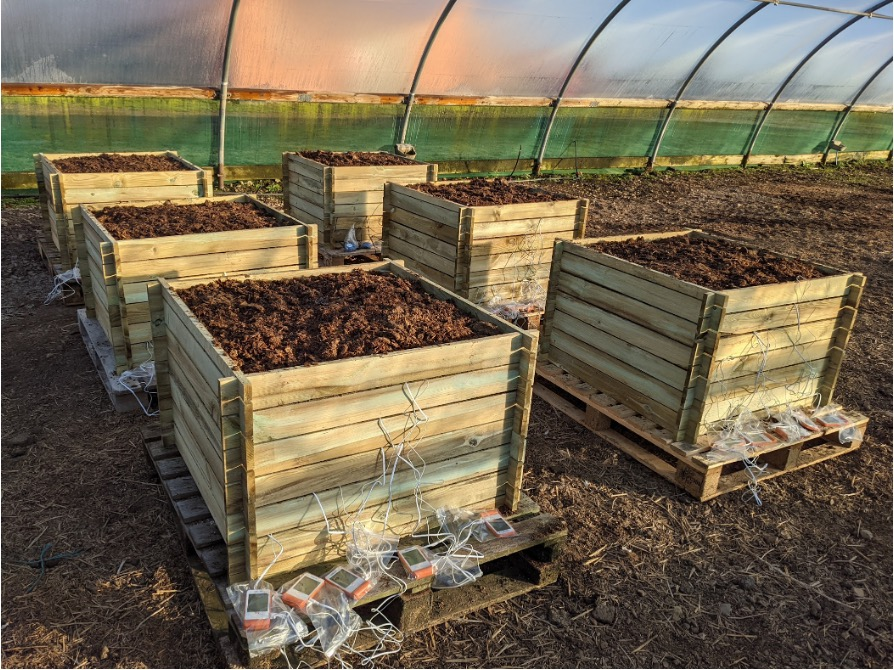
\includegraphics[width=\textwidth]{Figures/heaps.jpg}\\
	\end{column}
	\begin{column}{0.5\textwidth}
	\centering
\begin{itemize}
	\item temperature
	\item pH
	\item moisture content
	\item microbiota
	\item control sample - day 0, before making heaps
\end{itemize}
	\end{column}
\end{columns}
\end{frame}
\begin{frame}{AMR genes}
\begin{columns}
\begin{column}{0.5\textwidth}
	Genes targeted by rtPCR:
\scriptsize
\begin{itemize}
	\item AY1(16s rRNA) - host gene
	\item AY293(inti11) - Integron, related to HGT
	\item AY24(strB) - aminoglycosides
	\item AY456(qepA) - quinolone
	\item AY459(qnrD) - quinolone
	\item AY242(sul1) - sulfonamide
	\item AY577(tetR) - tetracycline
	\item AY284(dfrA1) - trimethoprim
	\item AY595(vanA) - vancomycin
	\item AY56(ermB1) - macrolide/MLSB
	\item AY184(satA)  - virginiamycin assoc.
	\item AY466(mcr1) - other (interesting dynamics).
\end{itemize}
\end{column}
\begin{column}{0.5\textwidth}
	Sampling locations:
	\begin{itemize}
		\item Top
		\item Top Corner (TC)
		\item Upper Middle (UM)
		\item Core
		\item Lower Middle (LM)
		\item Bottom Corner (BC)
	\end{itemize}
		\centering
		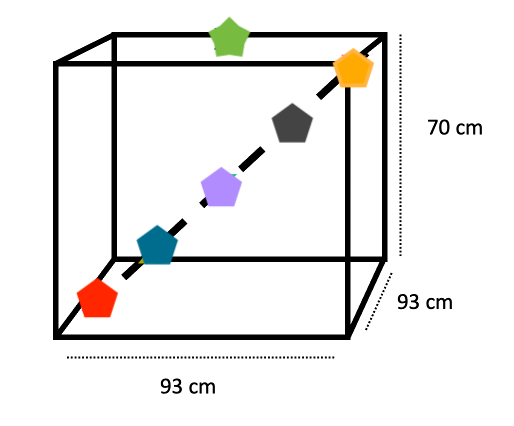
\includegraphics[width=0.6\textwidth]{Figures/Colour_coded_probes.png}\\
\end{column}
\end{columns}
\end{frame}
%%%%%%%%%%%%%%%%%%%%%%%%%%%%%%%%%%%%%%%%%%%%%%%%%%%%%%%%%%%%%%%%%%%%%%%%%%%%%%%%%%%%%%%%
\section{Experimental data informs models}
\subsection{Data from composting experiment}
\begin{frame}{Temperature in compost heaps}
\centering
	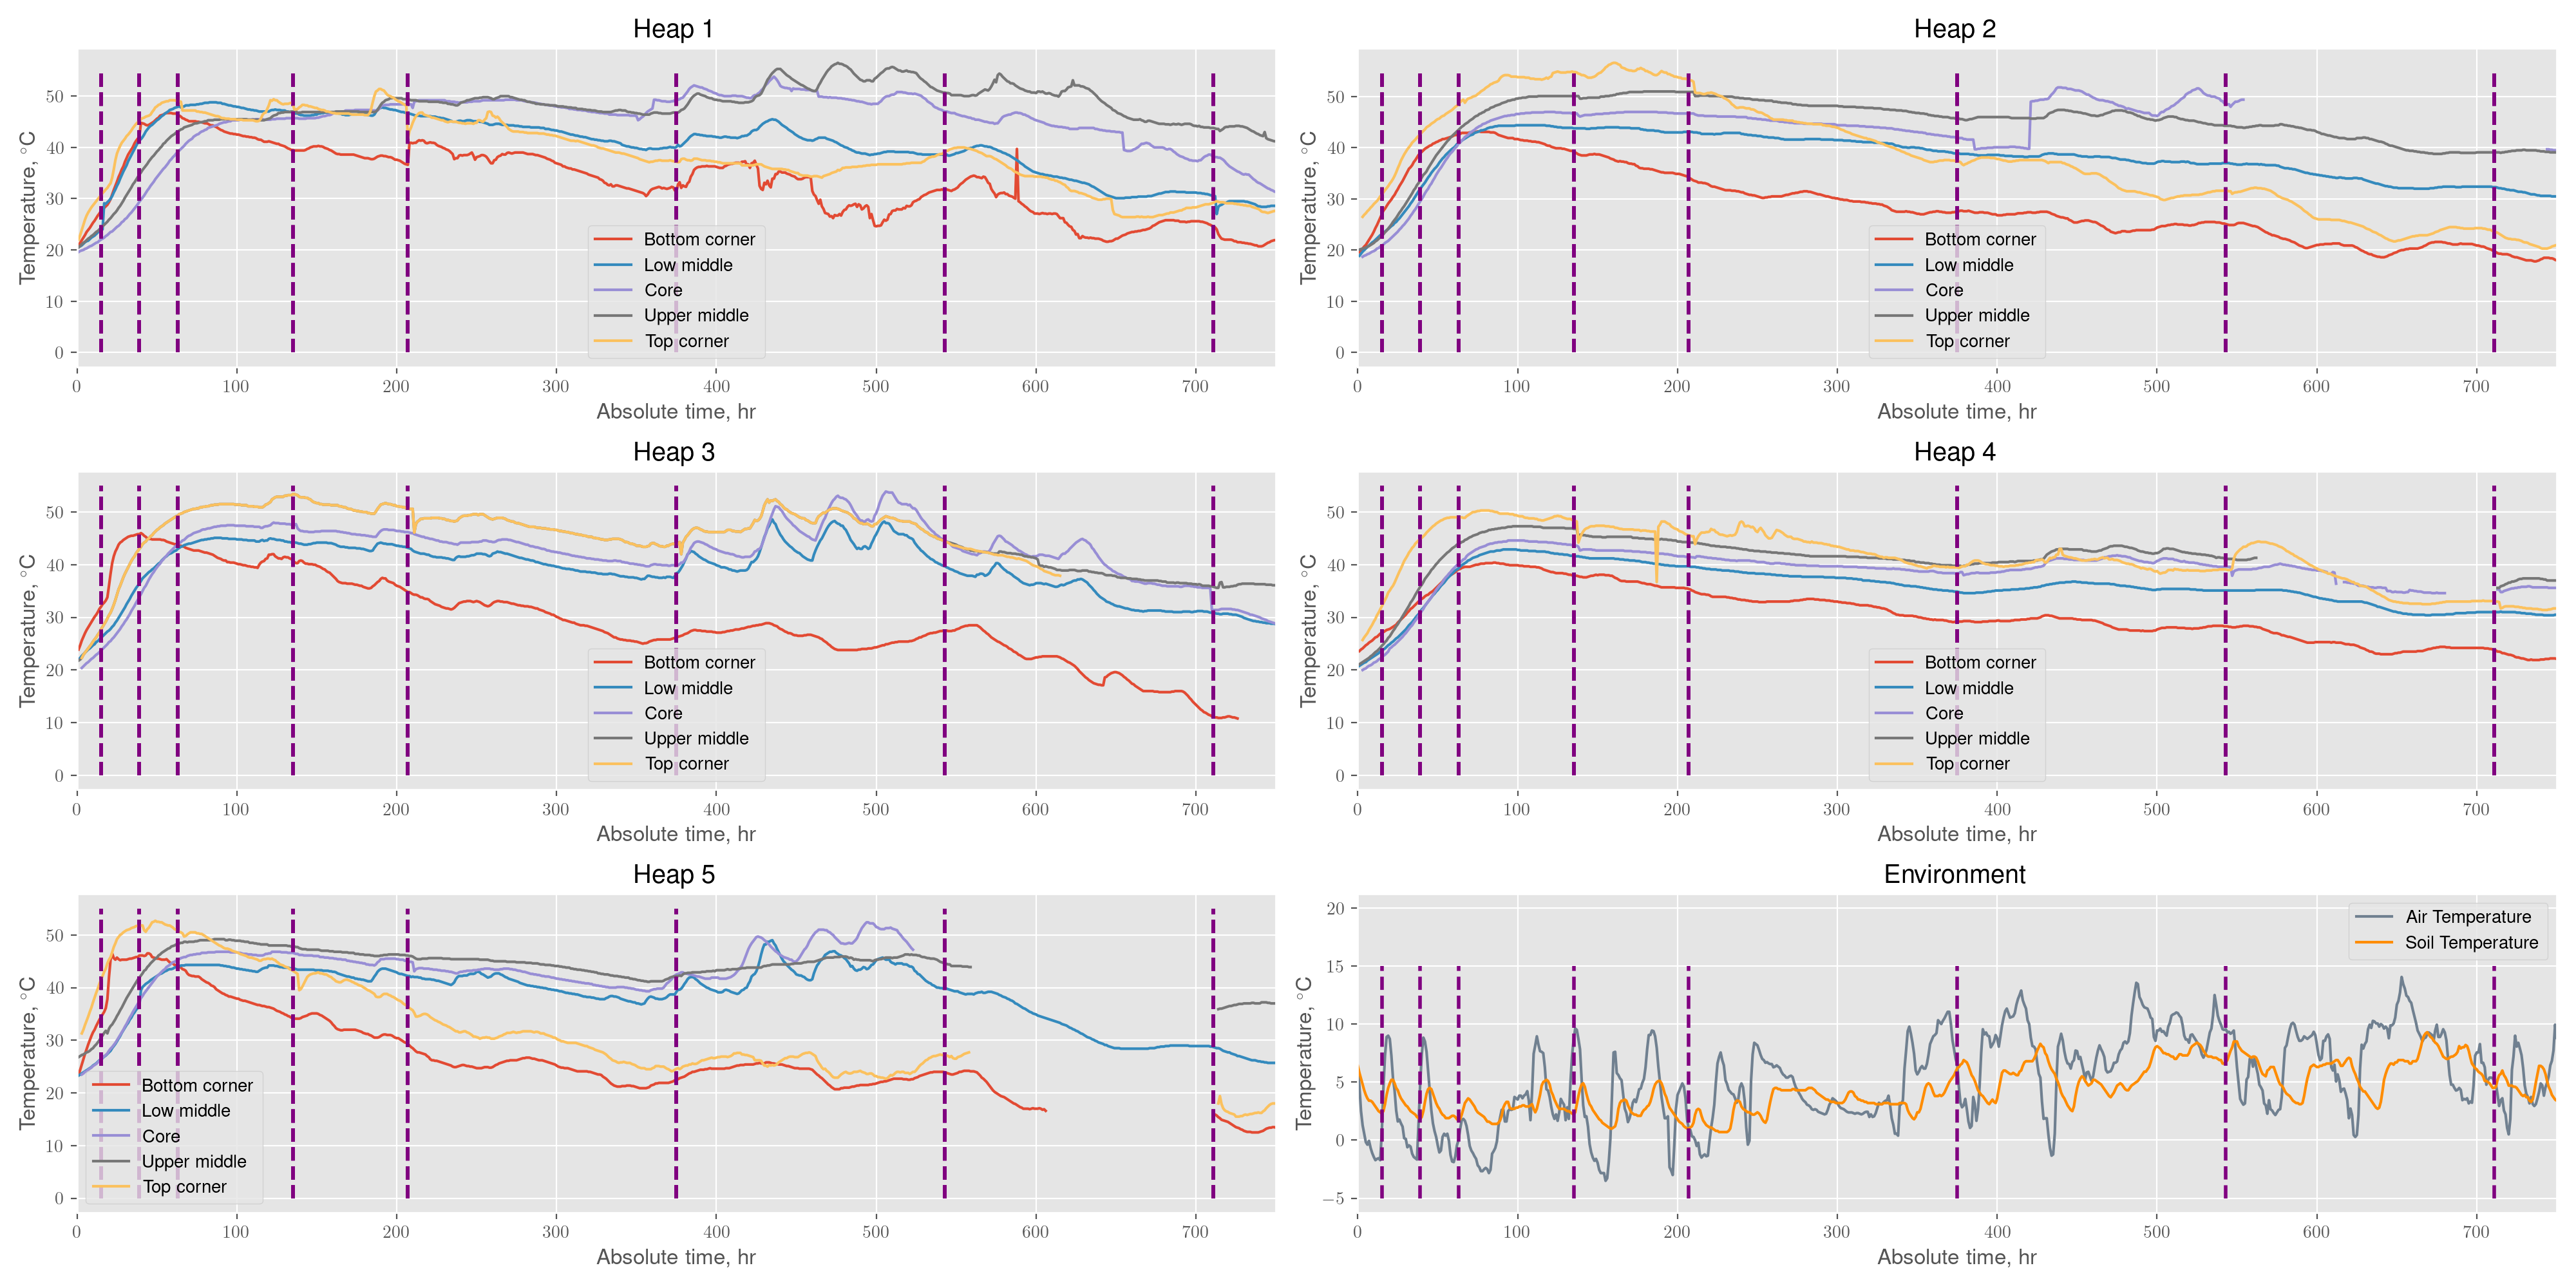
\includegraphics[width=\textwidth]{Figures/Temperatures_per_heap_crop.png}\\
	Vertical lines: times when microbiome sample was taken.
\end{frame}
\begin{frame}{Temperature gradients}
\centering
	\includegraphics[width=\textwidth]{Figures/all_heaps_temperature.png}\\
\end{frame}
\begin{frame}{pH in compost heaps}
\centering
	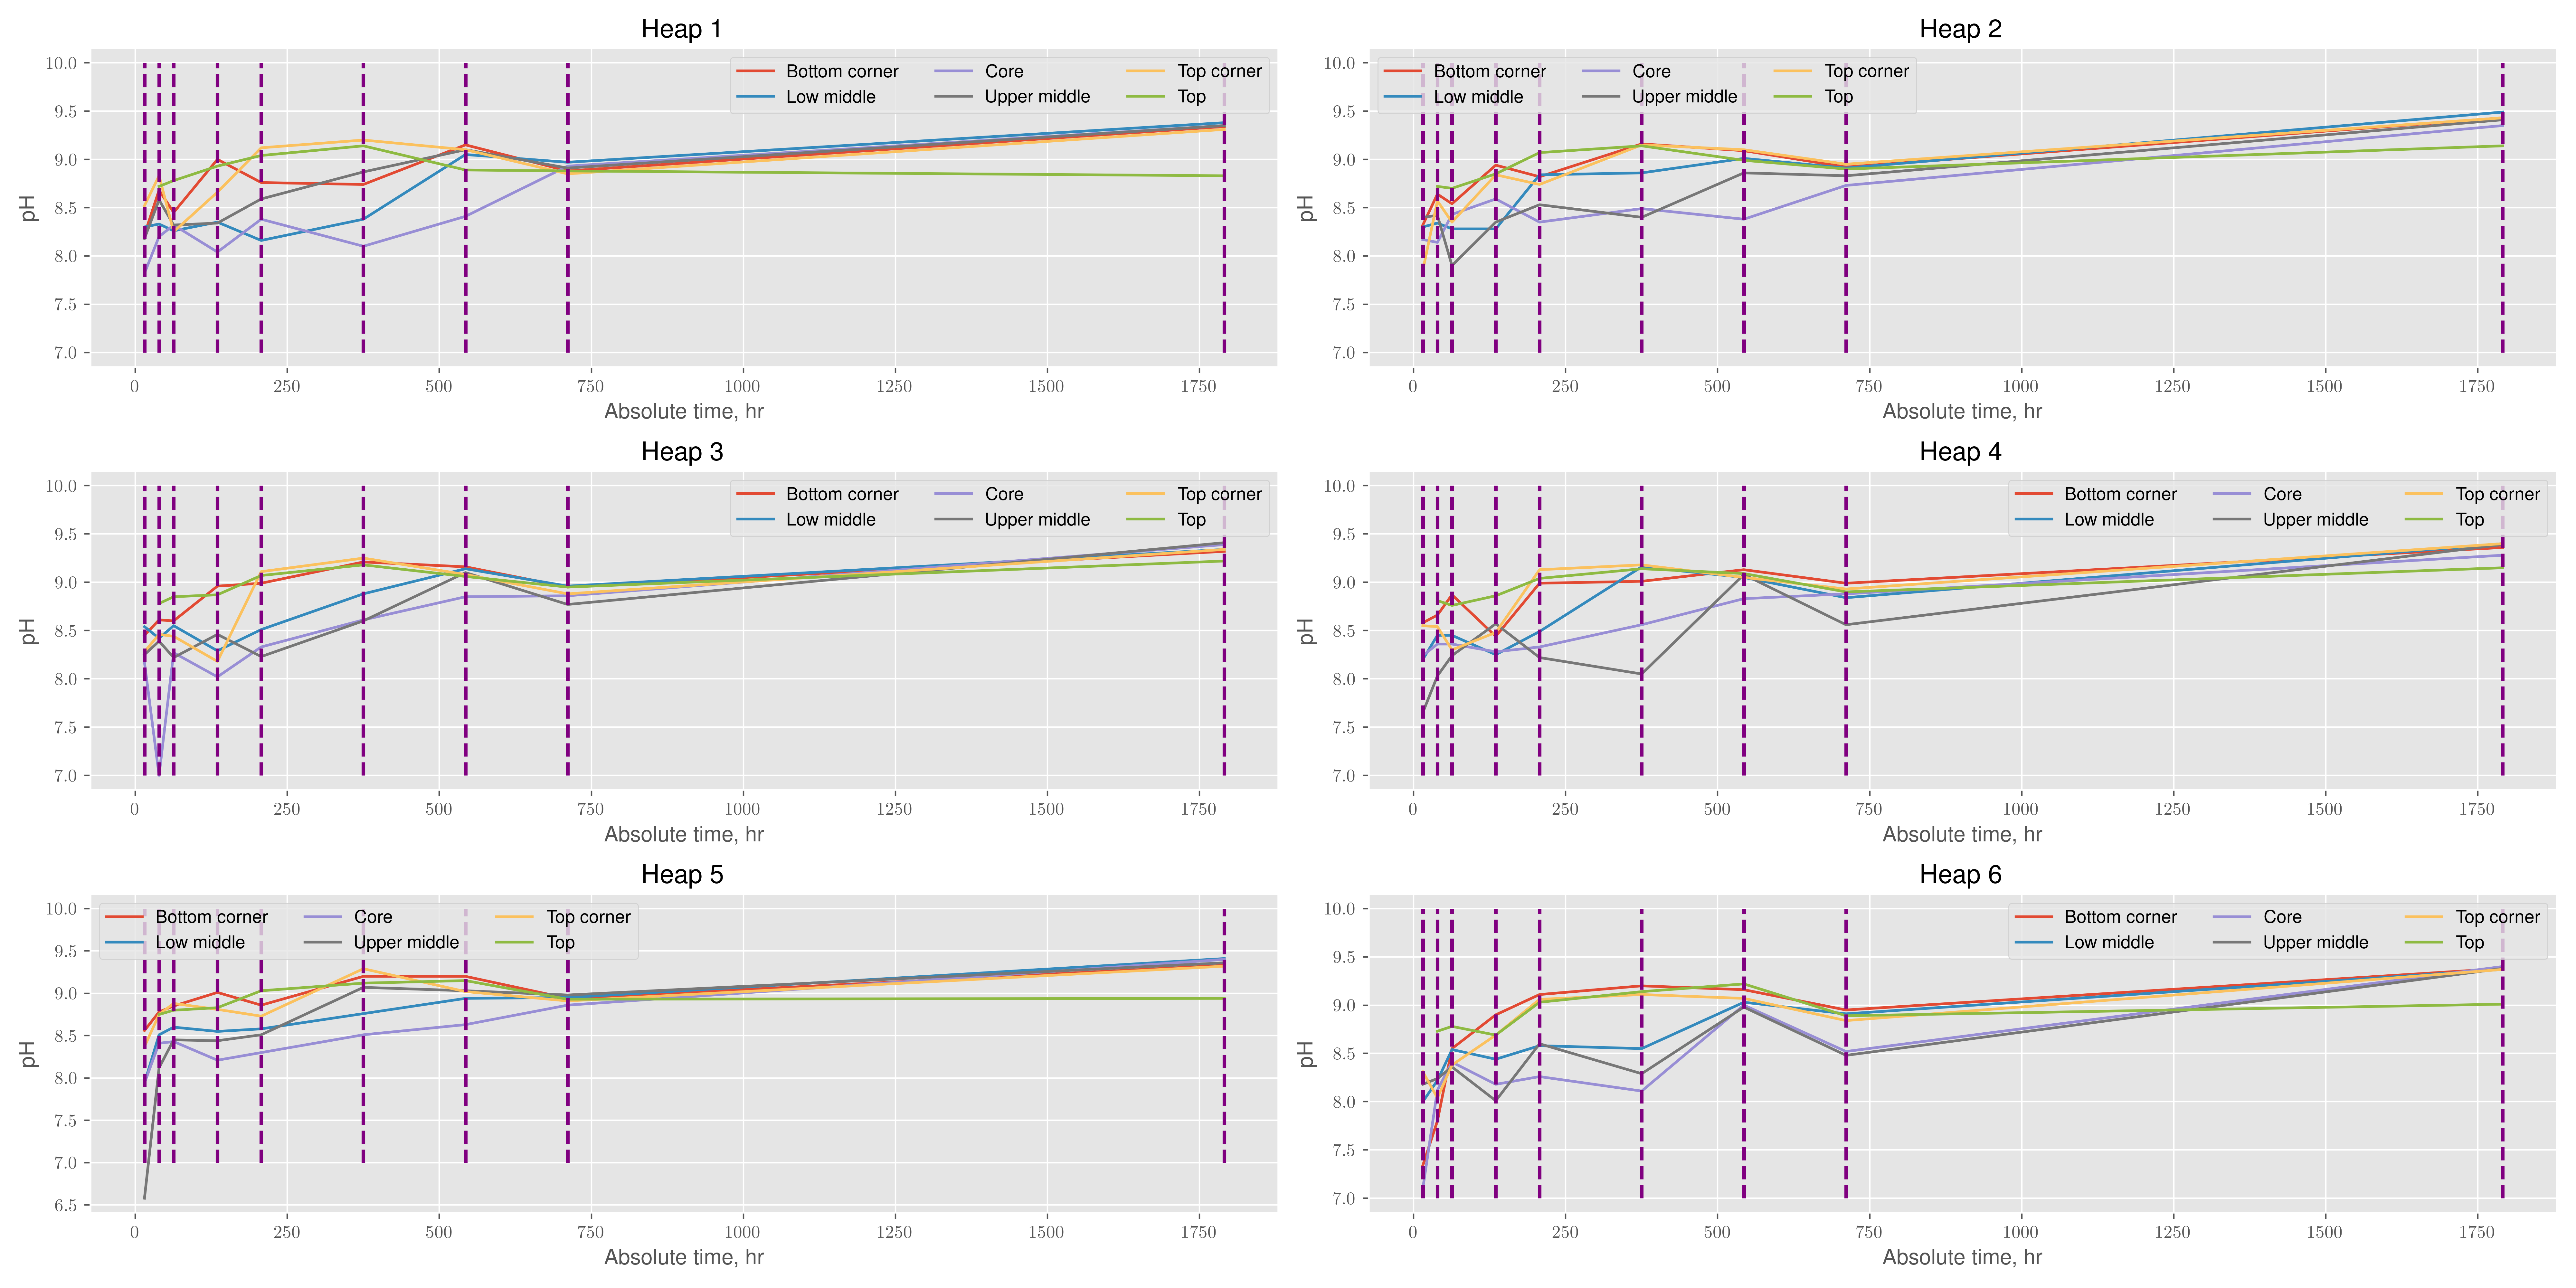
\includegraphics[width=\textwidth]{Figures/ph_per_heap.png}\\
	Vertical lines: times when microbiome sample was taken.
\end{frame}
\begin{frame}{Moisture content in compost heaps}
\centering
	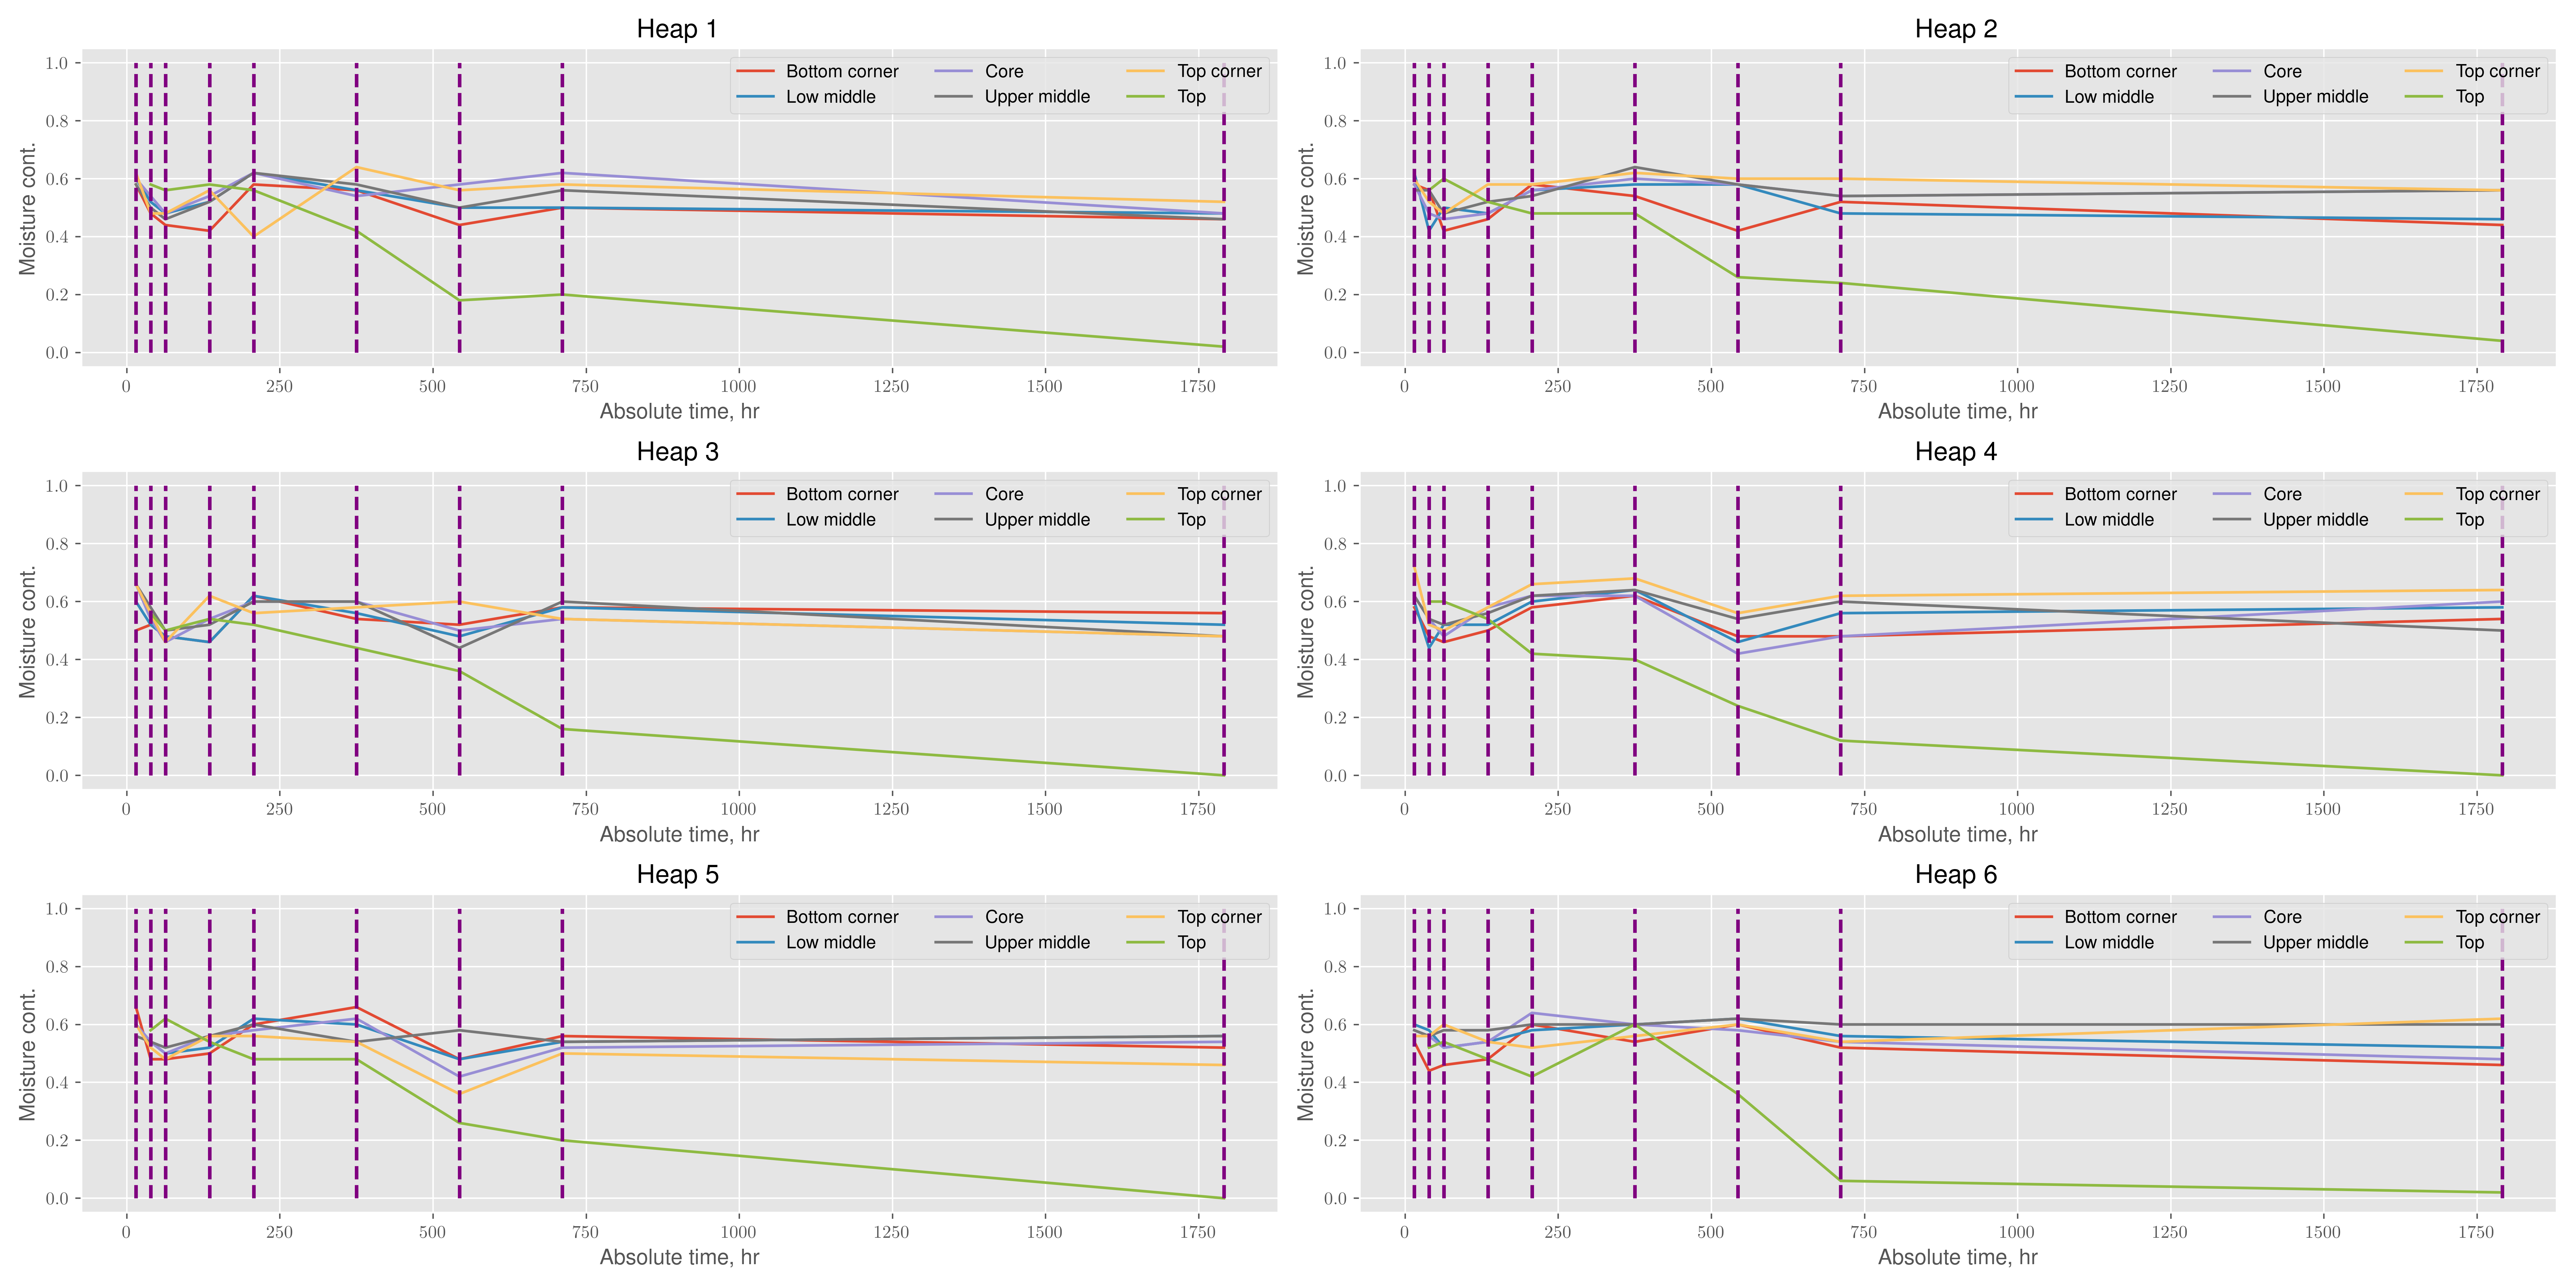
\includegraphics[width=\textwidth]{Figures/mc_per_heap.png}\\
	Vertical lines: times when microbiome sample was taken.
\end{frame}
\begin{frame}{Interpolation across time}
\centering
	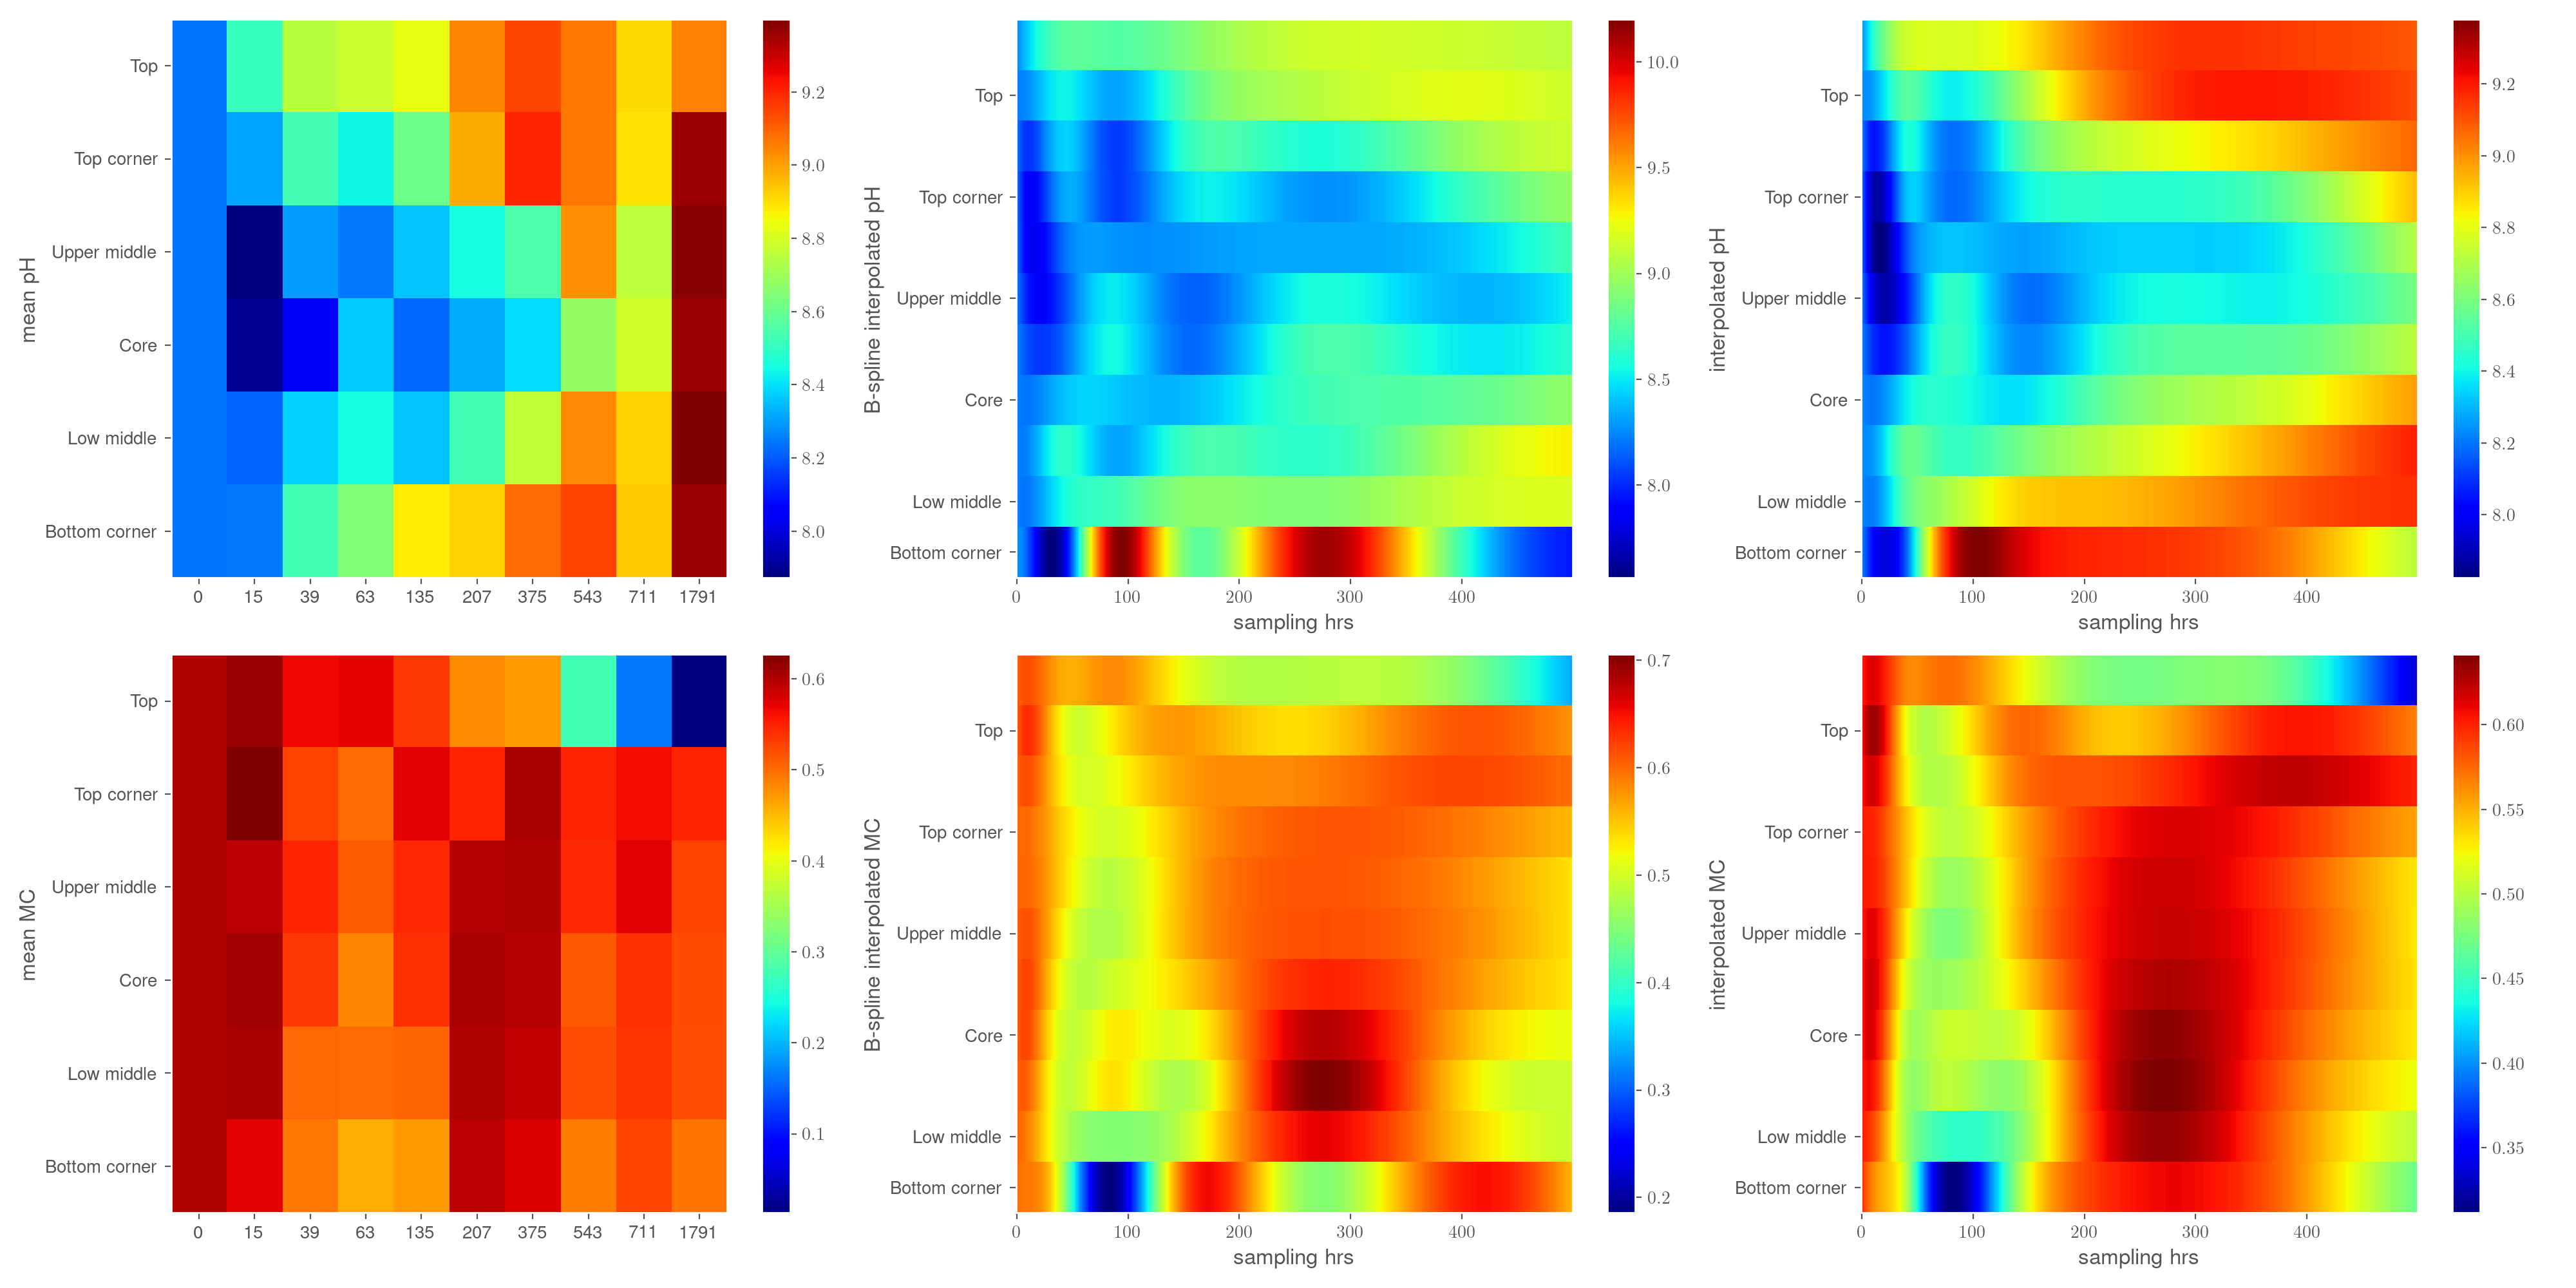
\includegraphics[width=\textwidth]{Figures/interpolation_ph_mc.png}\\
\end{frame}
\subsection{Working with AMR genes}
\begin{frame}{Computing relative abundances}
Pre-processing:
\begin{itemize}
	\item For each sampling location 6 biological replicates
	\item Each replicate is split into 3 technical replicates
	\item The smaller the cycle threshold (CT), the more abundant the gene
	\item If primer temperature between the three replicates has large difference = outlier
	\item If CT between the three replicates has large difference = outlier
	\item Use geometric mean of CT for three technical replicates
\end{itemize}
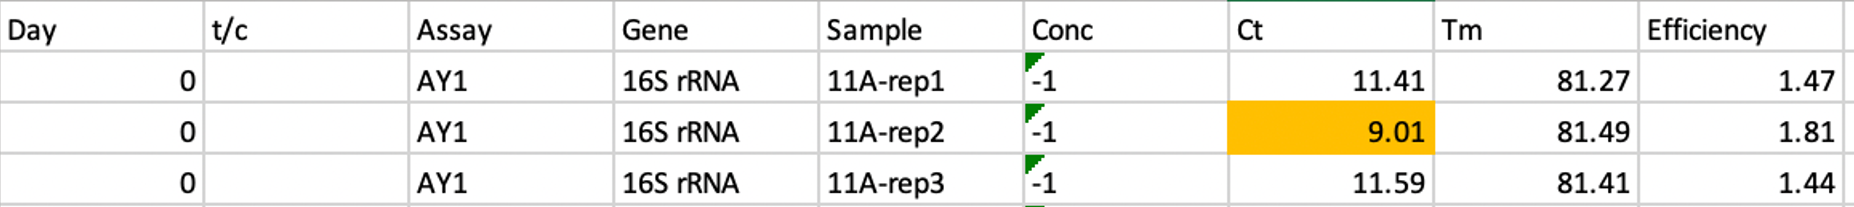
\includegraphics[width=\textwidth]{Figures/example_rtpcr.png}
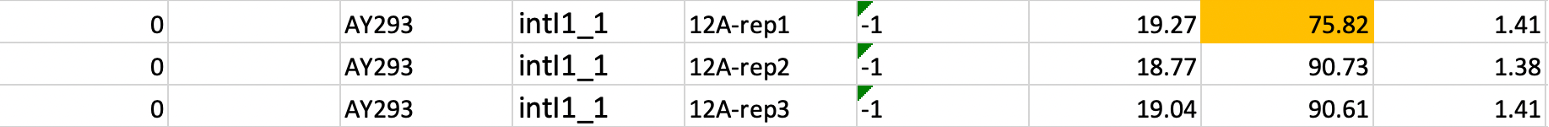
\includegraphics[width=\textwidth]{Figures/example_rtpcr_tm.png}
\end{frame}
\begin{frame}{Computing relative abundances}
Two methods to get relative abundance:
	\begin{itemize}
	\item Single delta method: with respect to the house gene (16S) of the same biological replicate:	
			\begin{align*}
			&\Delta C_{T}(\text{ARG}) = C_{T}(\text{ARG}) - C_{T}(\text{16S})\\
			& \text{RA}(\text{ARG}) = 2^{-\Delta C_{T}(\text{ARG})}
			\end{align*}
	\item Double delta method: the single delta of replicate compared to single delta in the control sample:
			\begin{align*}
			&\Delta \Delta C_{T}(\text{ARG}) = \Delta \Delta C_{T}(\text{target}) - \Delta \Delta C_{T}(\text{control}) \\
			& \text{RA}(\text{ARG}) = 2^{-\Delta \Delta C_{T}(\text{ARG})}
			\end{align*}
\end{itemize}
\end{frame}
\begin{frame}{Relative abundances of AMR genes}
Relative abundances computed using single delta method:
	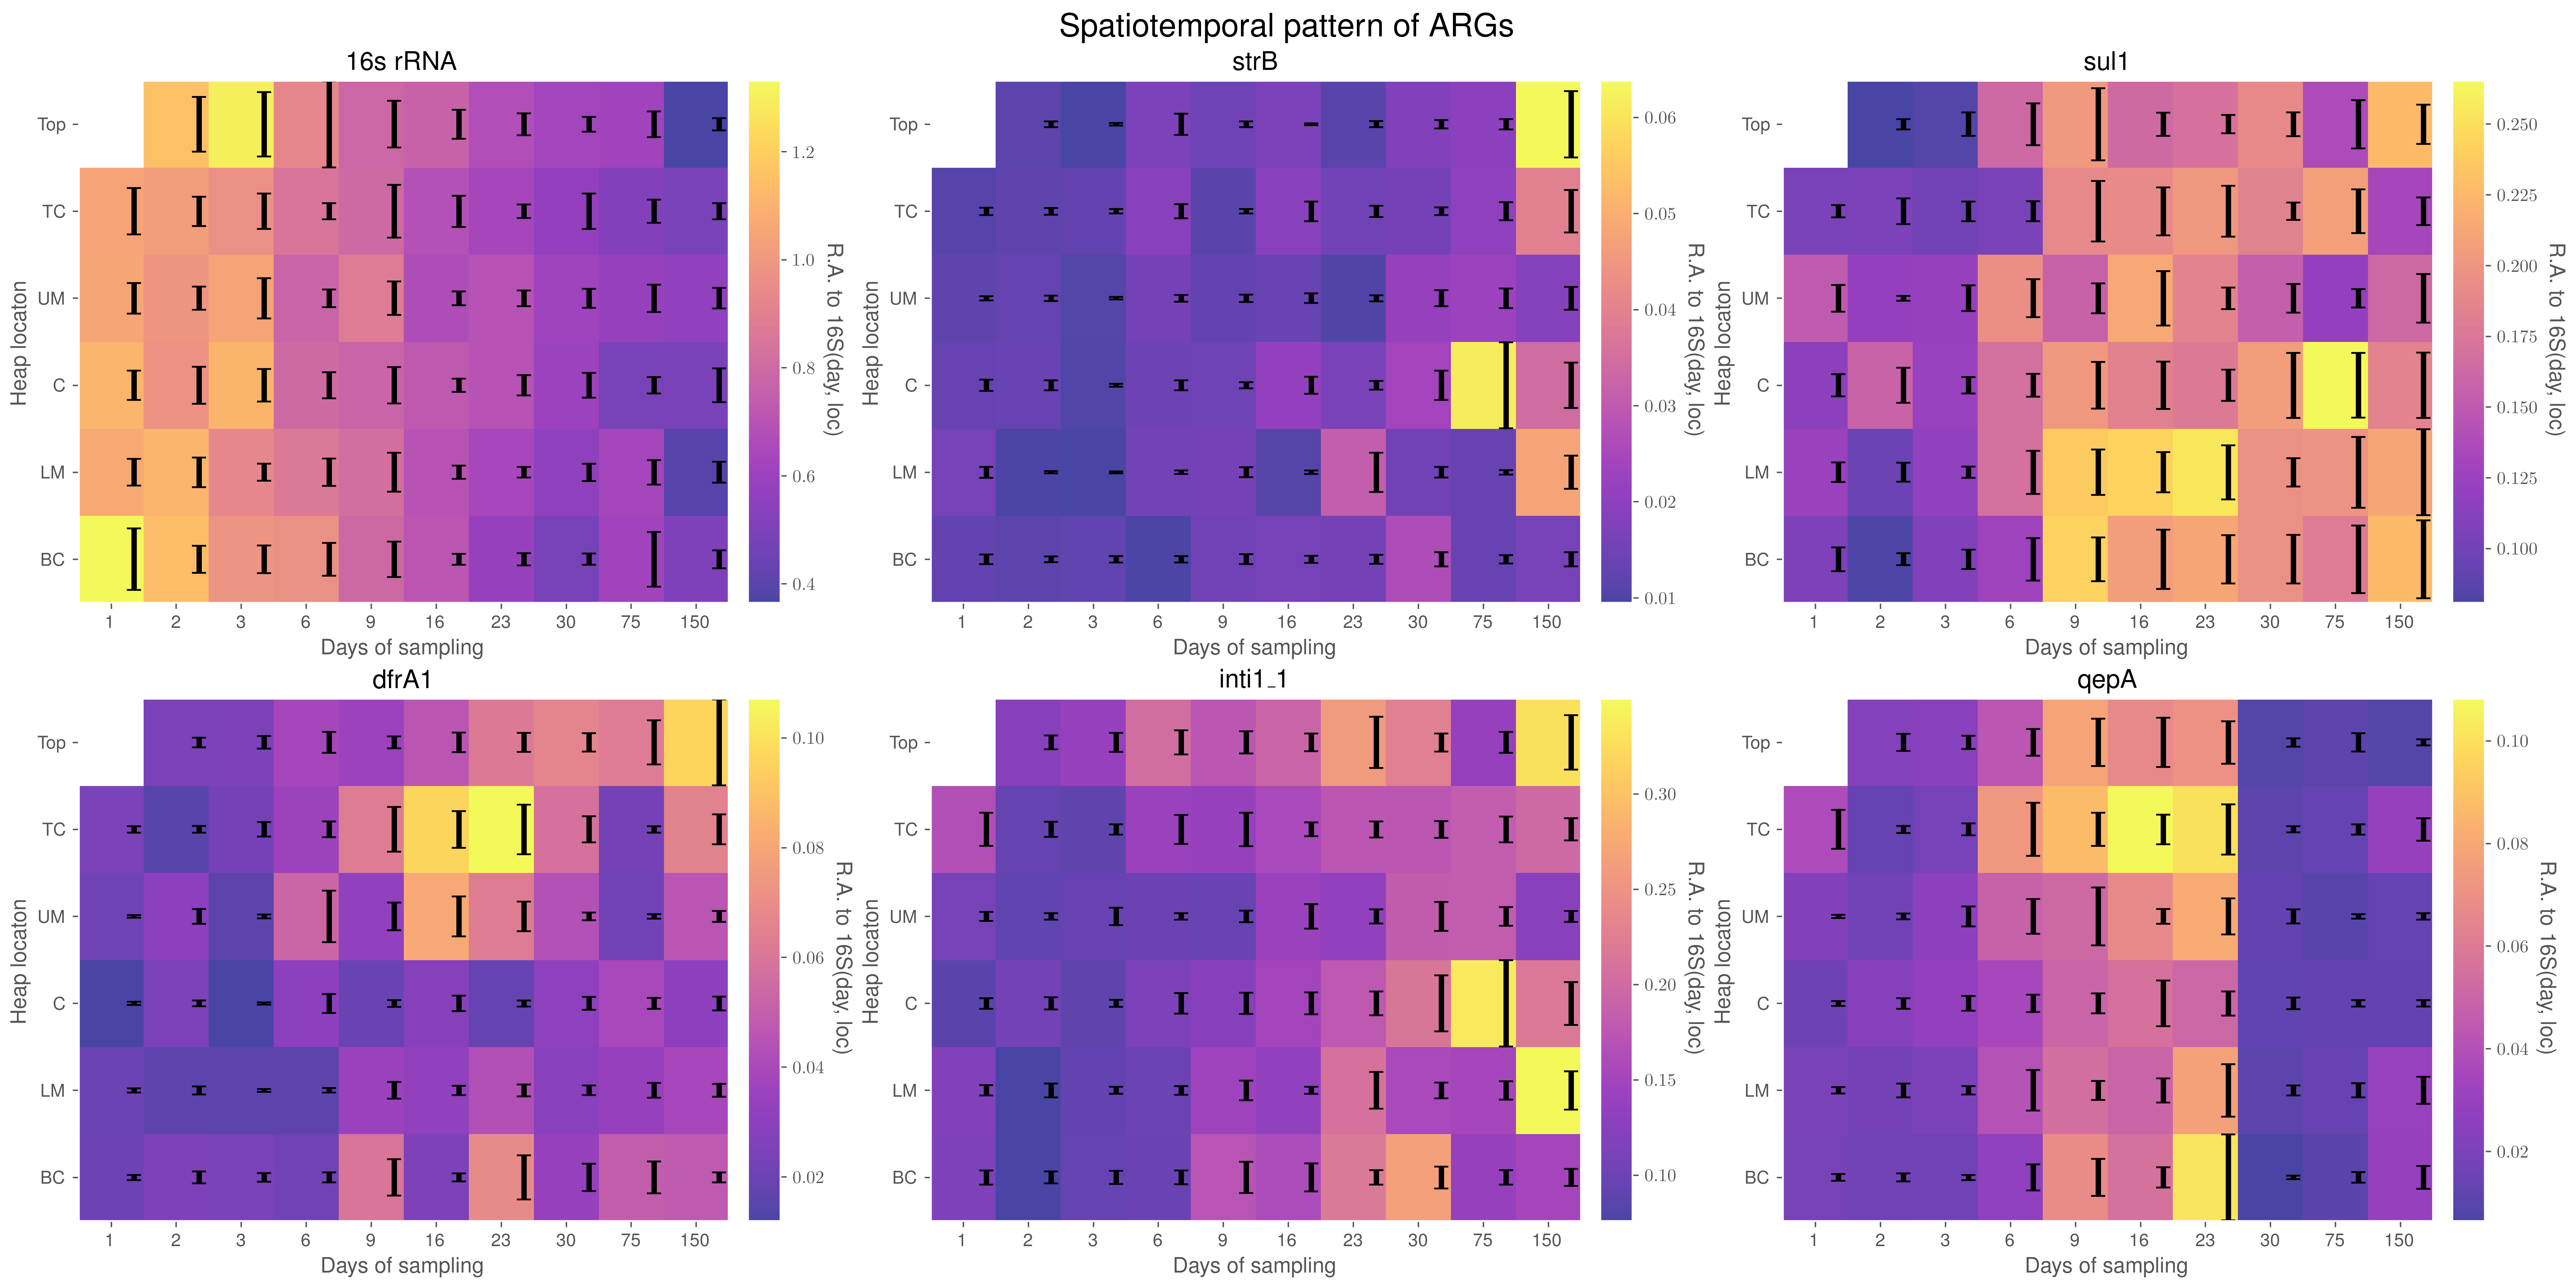
\includegraphics[width=\textwidth]{Figures/Sian_spatial_variation_first6_assays_with_errorbar.png}
\end{frame}
\begin{frame}{Relative abundances of AMR genes}
Relative abundances computed using single delta method:
	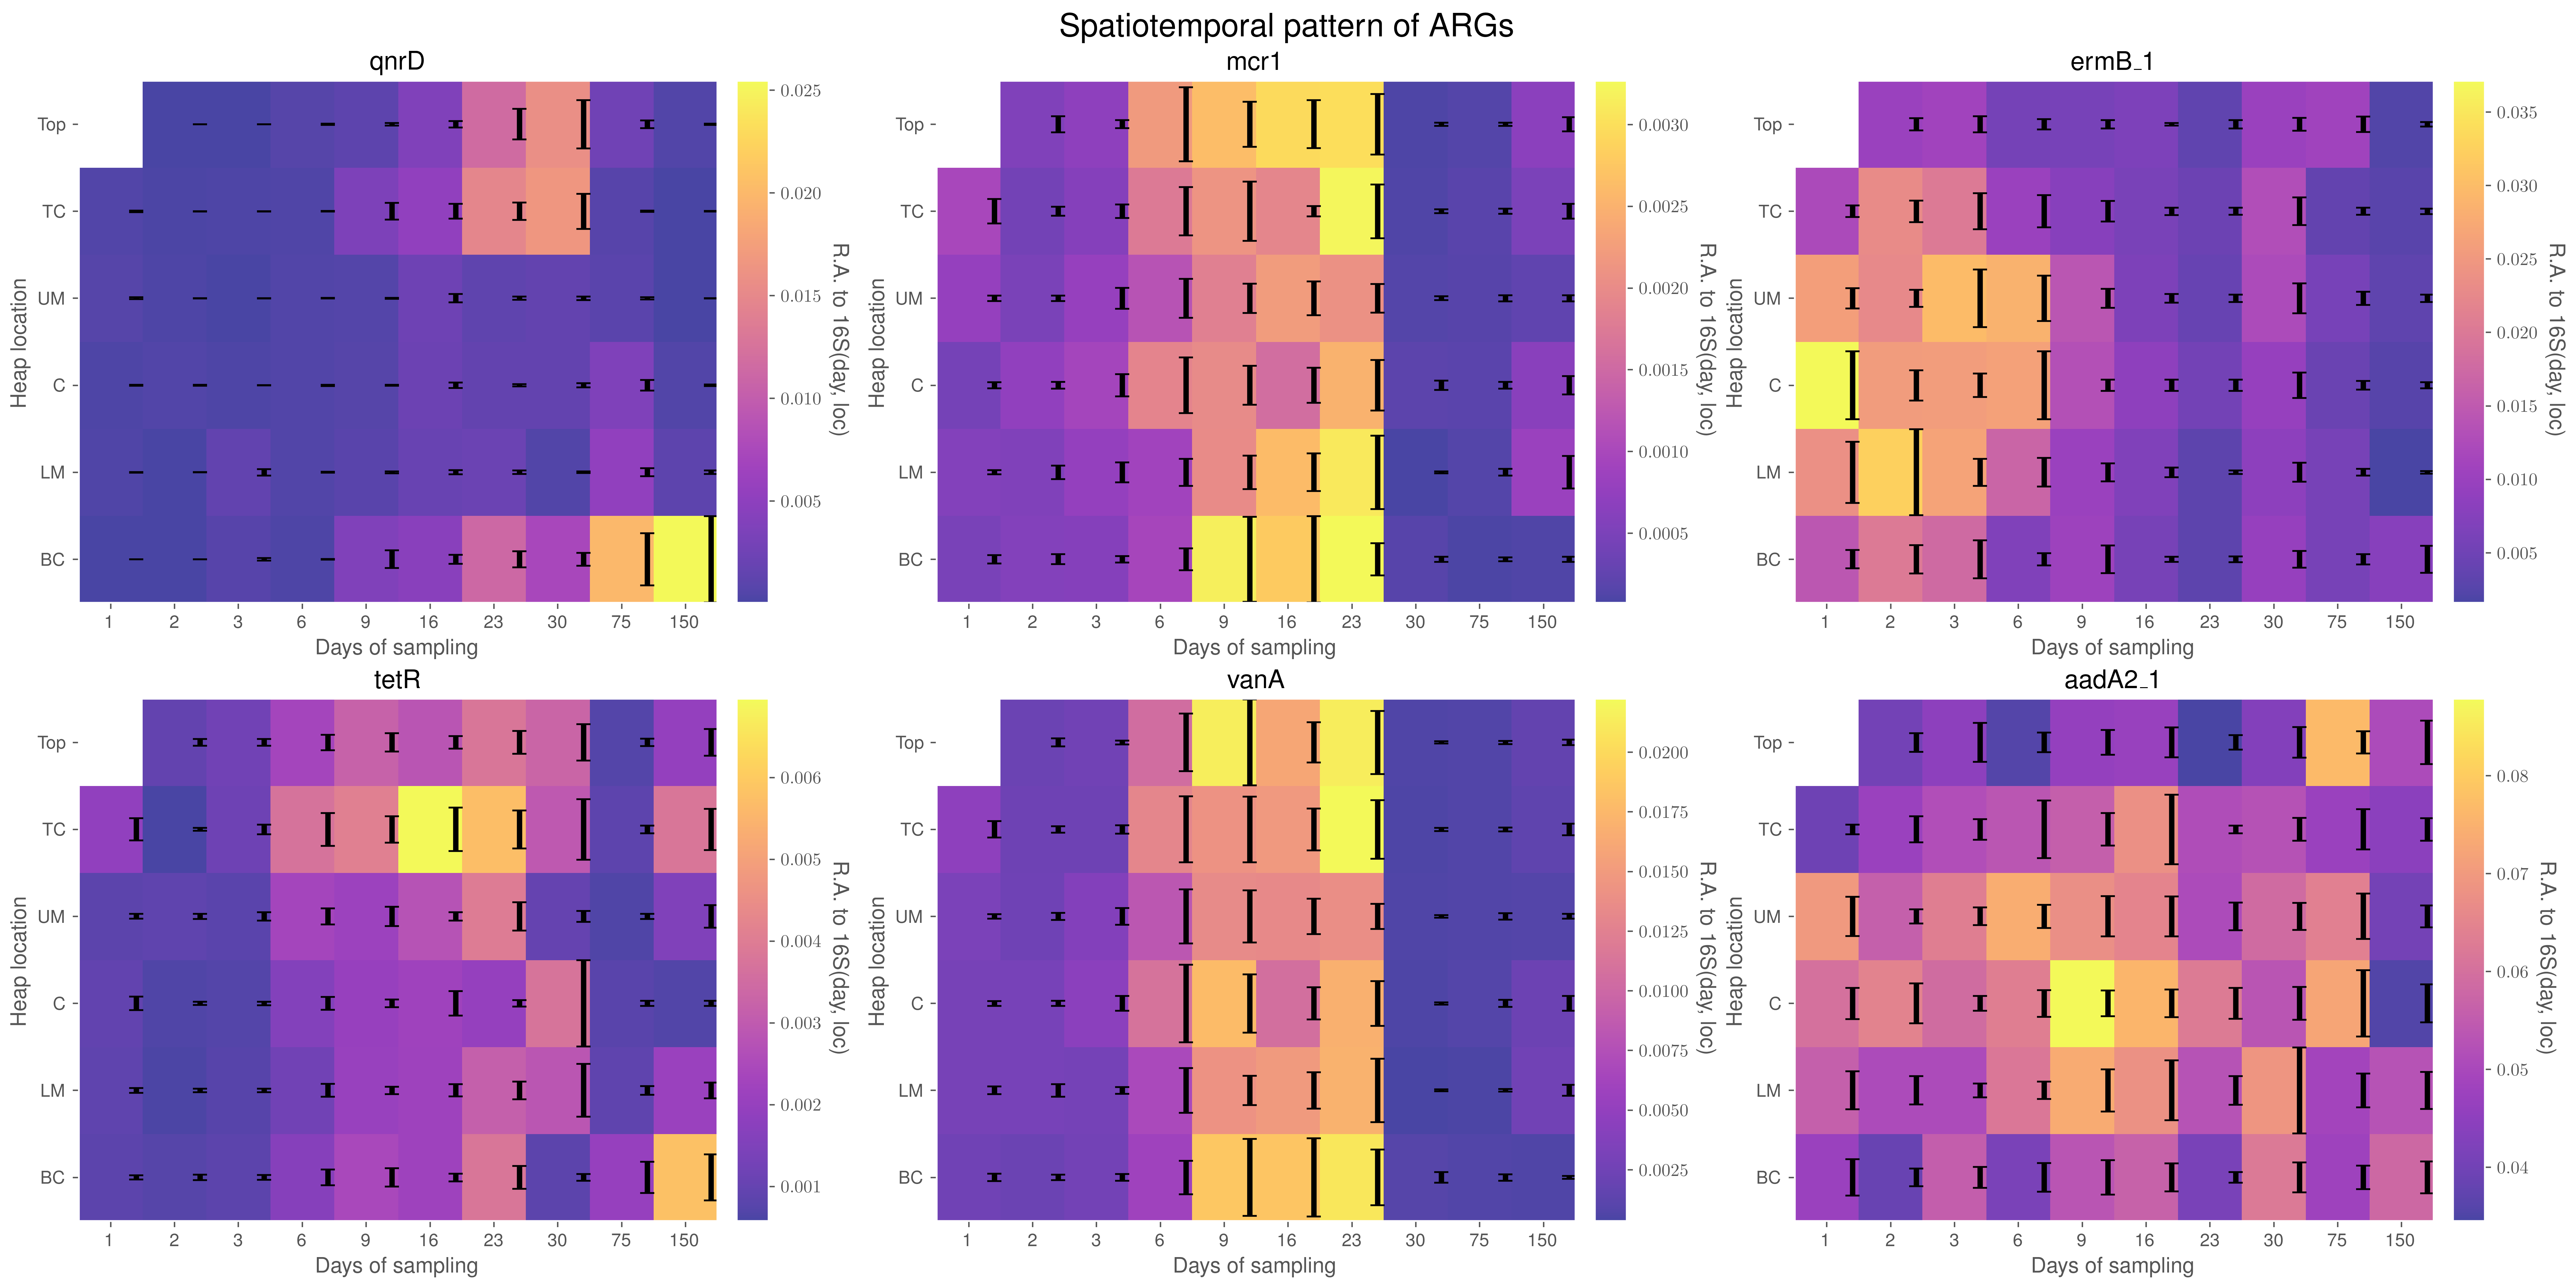
\includegraphics[width=\textwidth]{Figures/Sian_spatial_variation_second6_assays_with_errorbar.png}
\end{frame}
\begin{frame}{Different viewpoint}
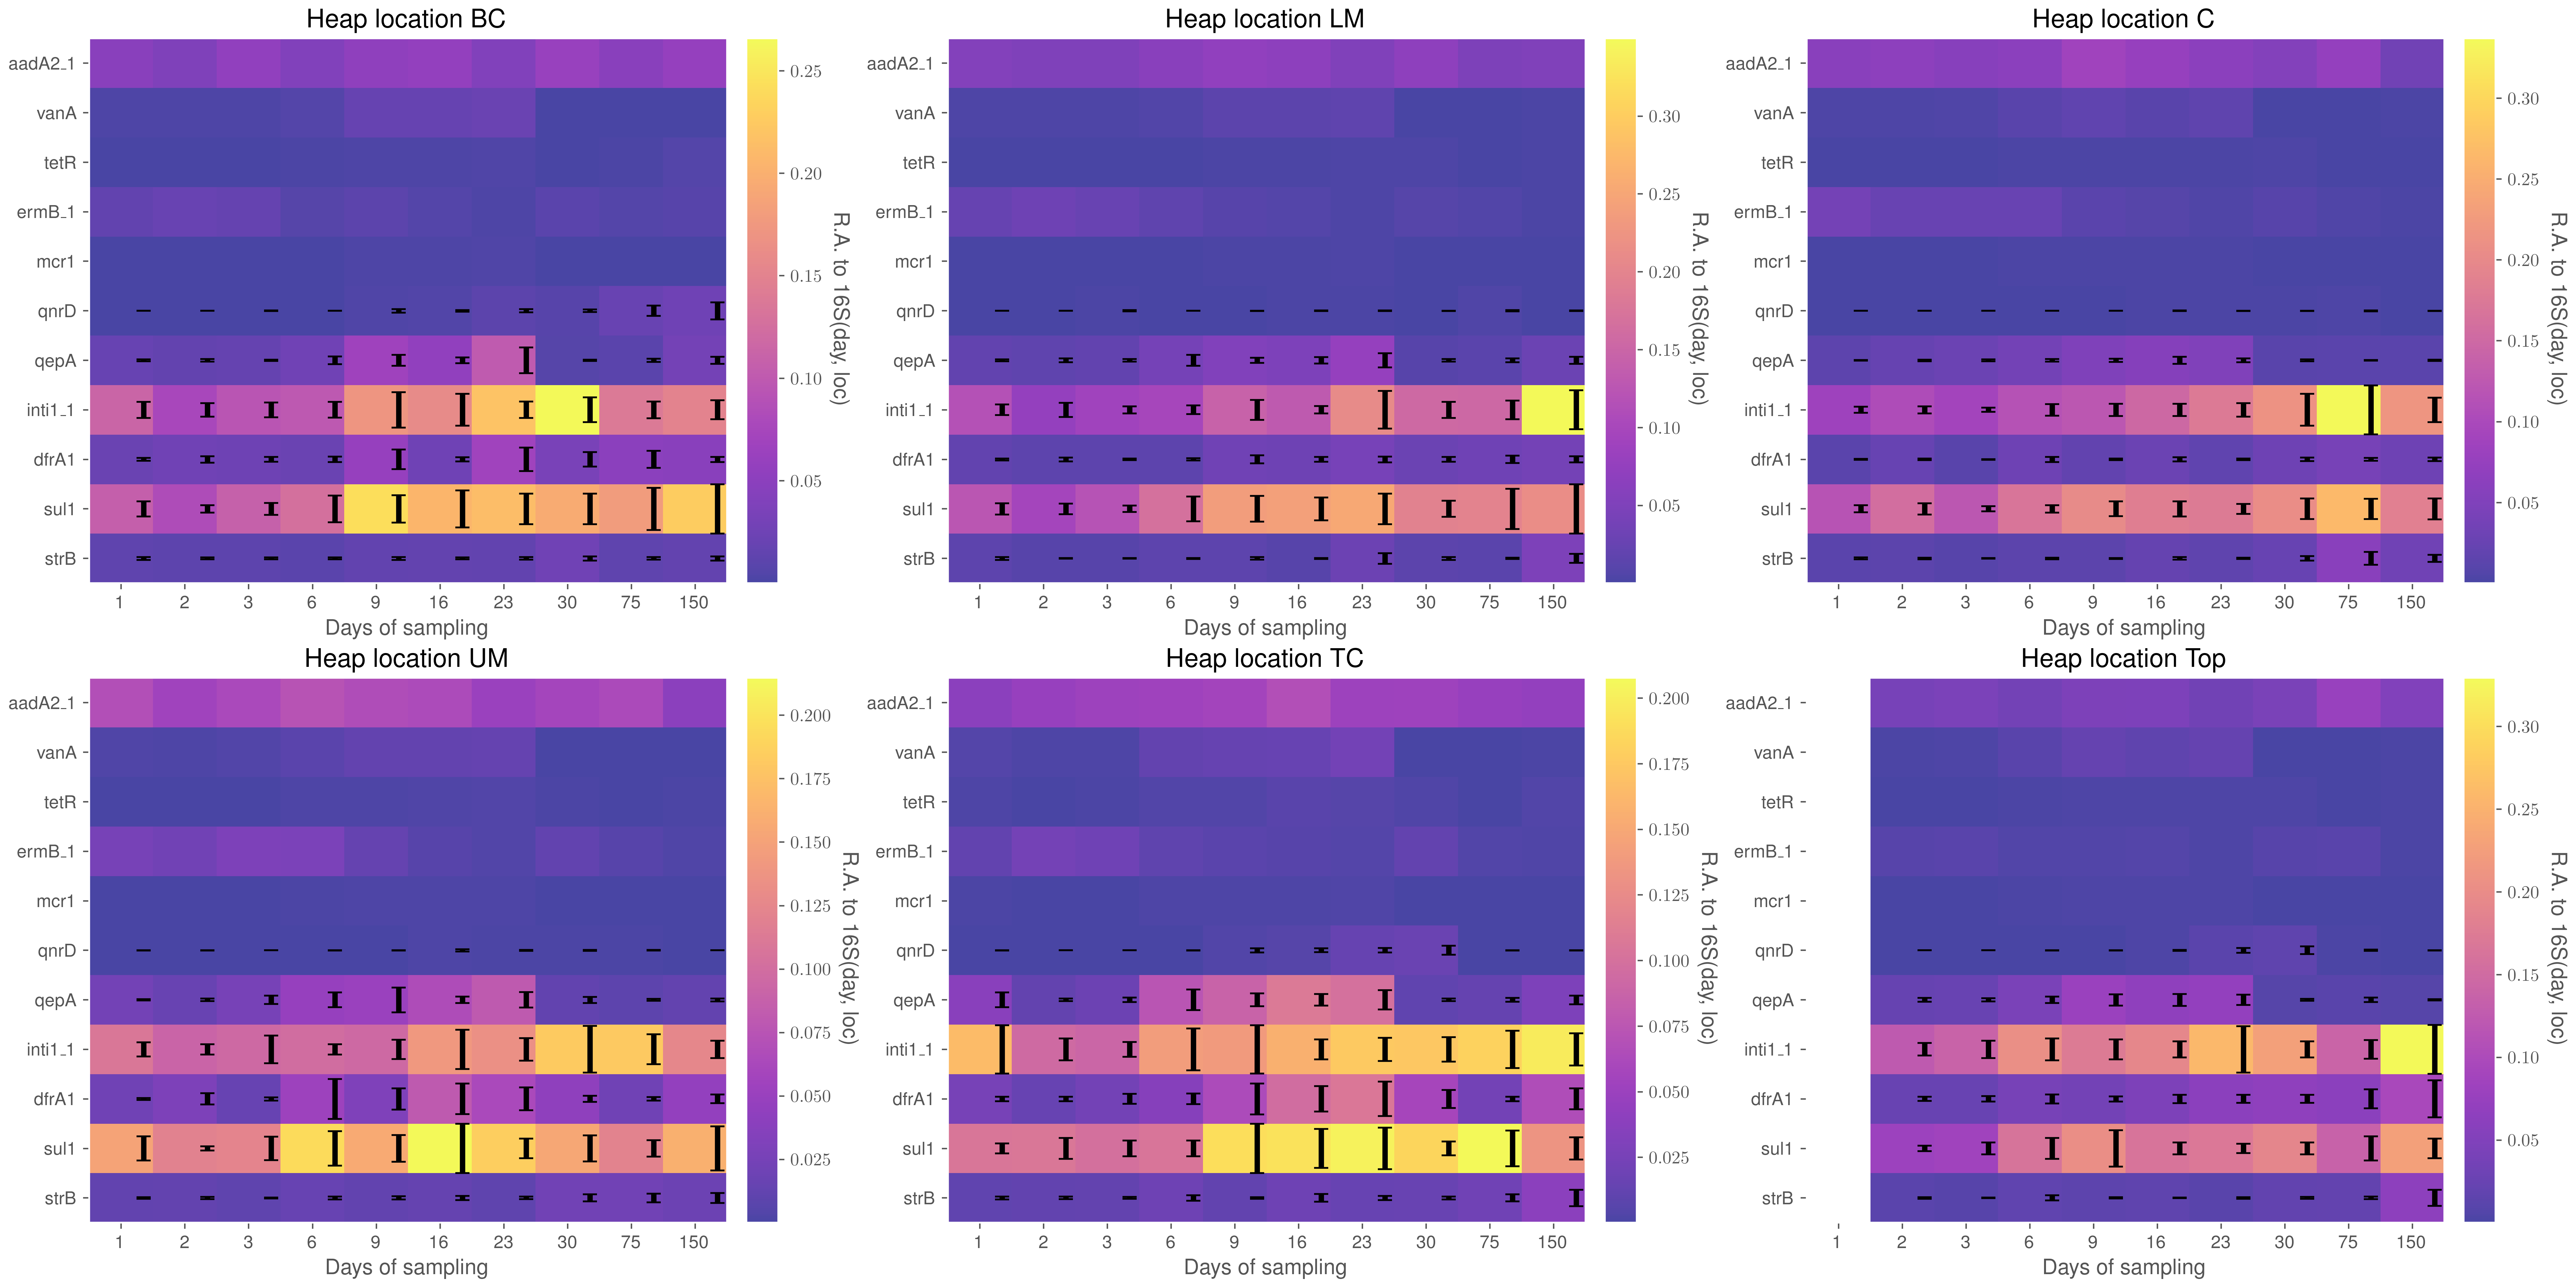
\includegraphics[width=\textwidth]{Figures/Sian_populations_in_positions_no_16s.png}
\end{frame}
\subsection{Searching for patters}
\begin{frame}{Hypothesis testing: location}
$\mathcal{H}0$: Distribution of RAs in "inner locations" of the heap (core, LM, UM) is stochastically equal to the distr. of RAs in "outer locations" (top, TC, BC).
	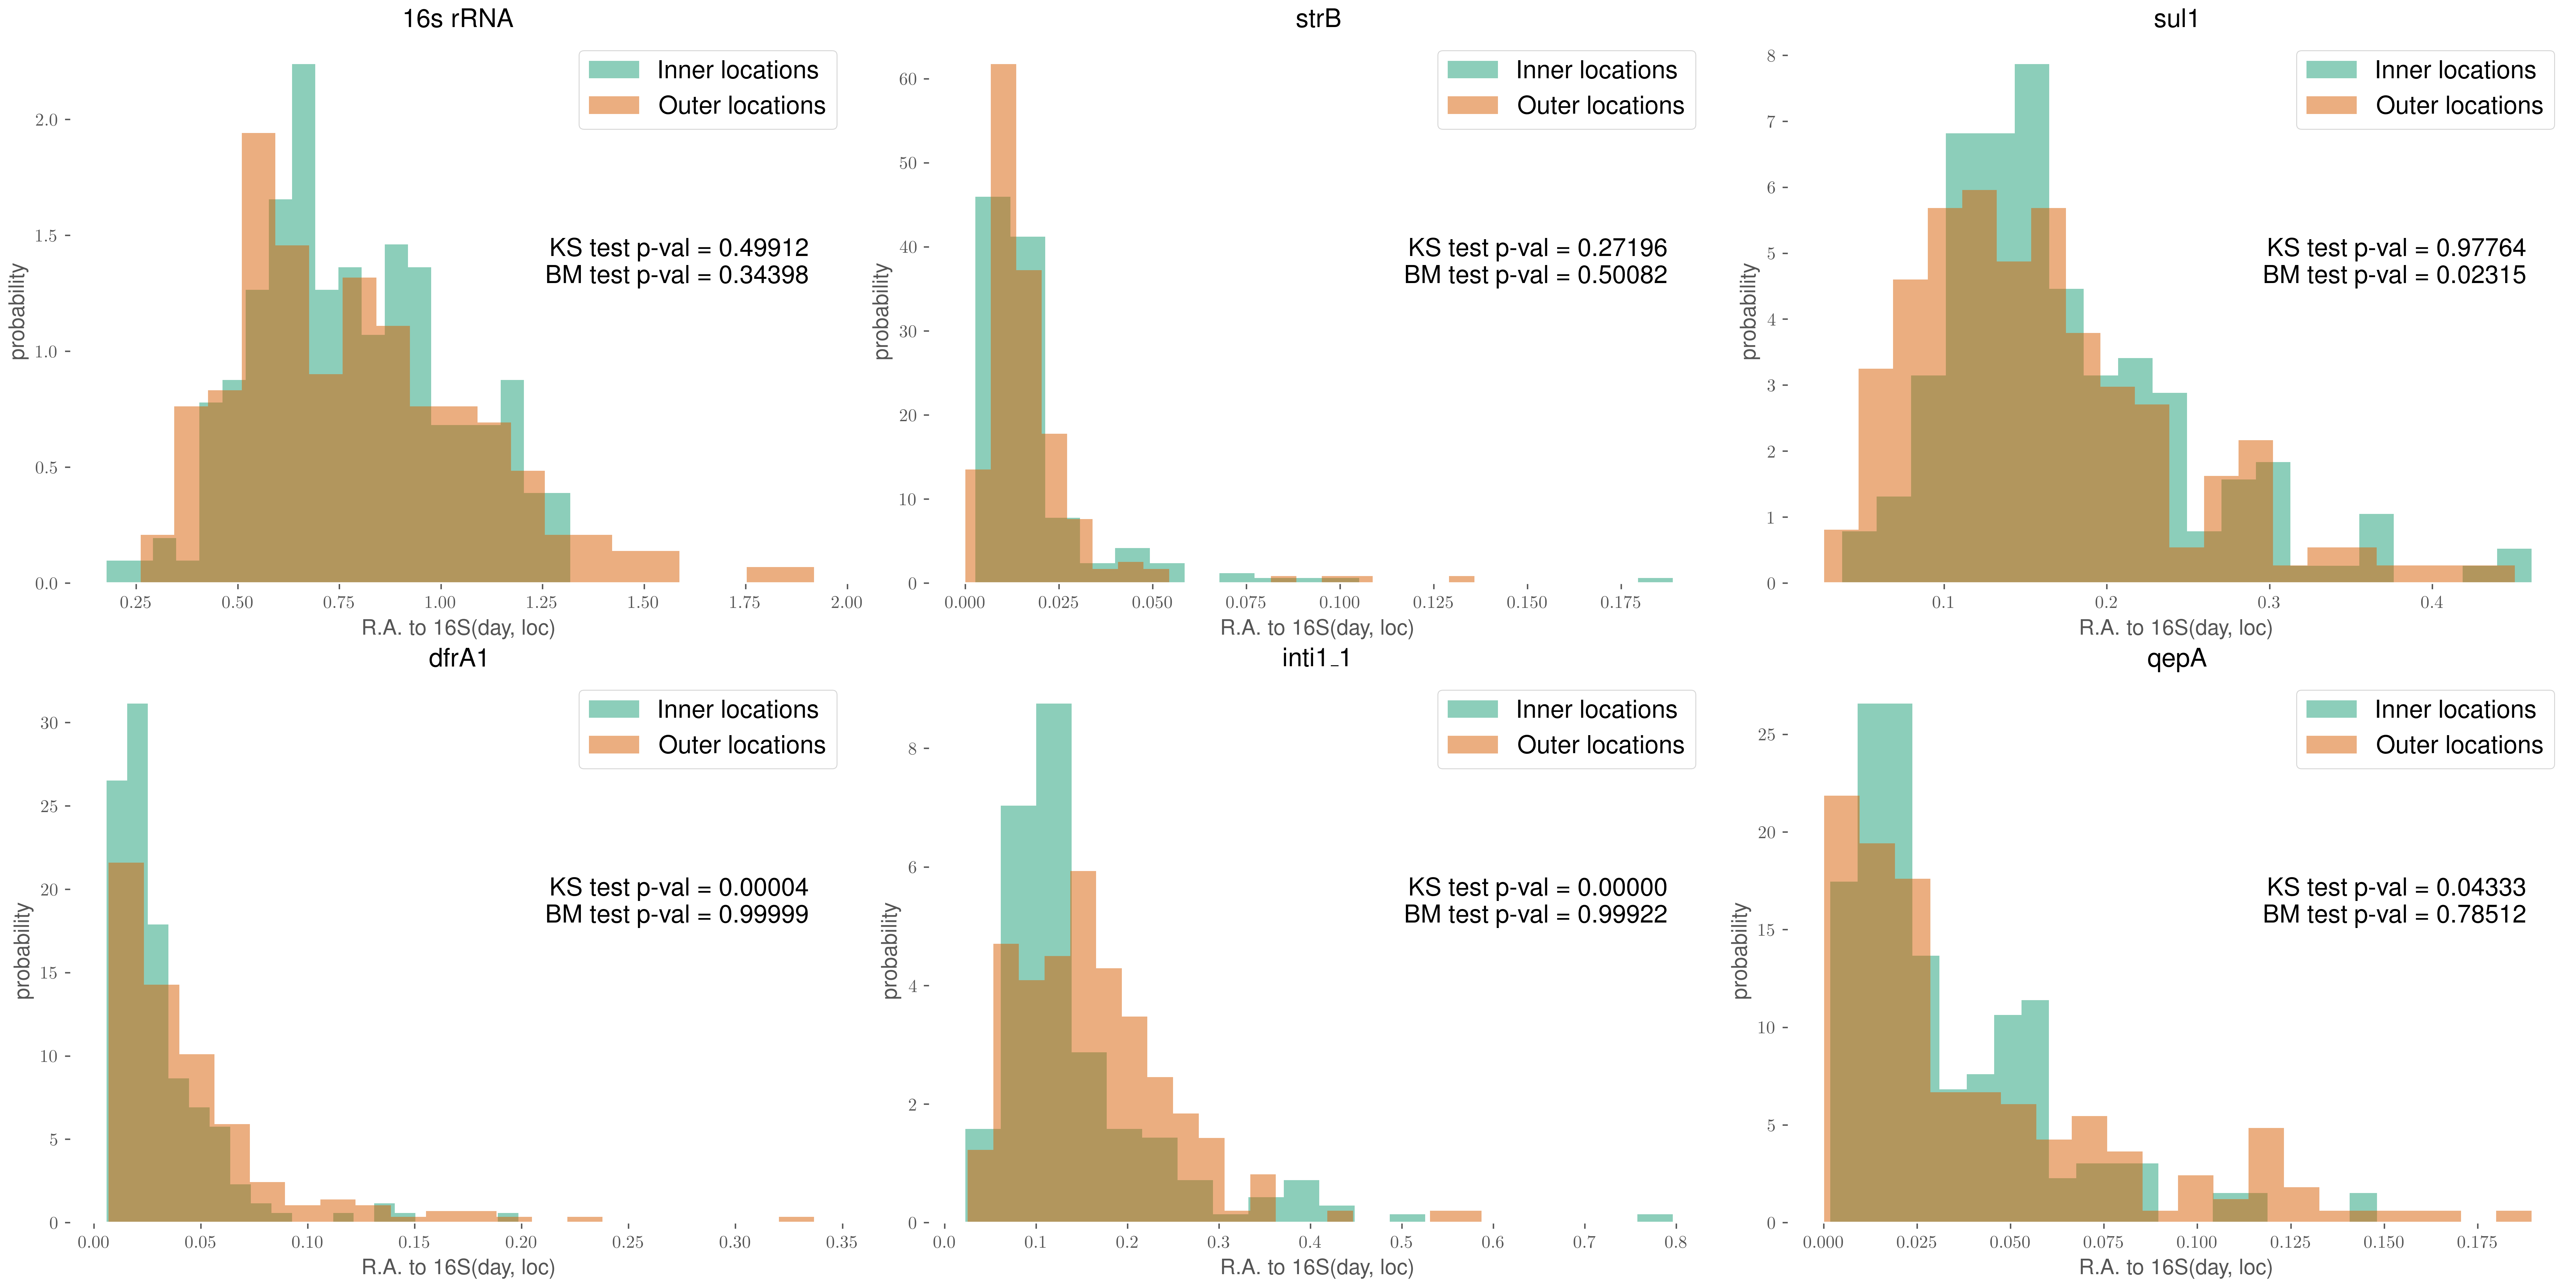
\includegraphics[width=\textwidth]{Figures/Sian_inner_vs_outer_hists_first_6_assays.png}
\end{frame}
\begin{frame}{Hypothesis testing: time}
Three stages of composting: mesophilic (M, days 1,2,3), thermophilic, (T, days 6,9,15), and cooling (C, days 23, 75, 150)
$\mathcal{H}0$: Distribution of RAs at one stage of the heap is stochastically equal to the  as RAs in the other stage. (3 pairwise tests):
	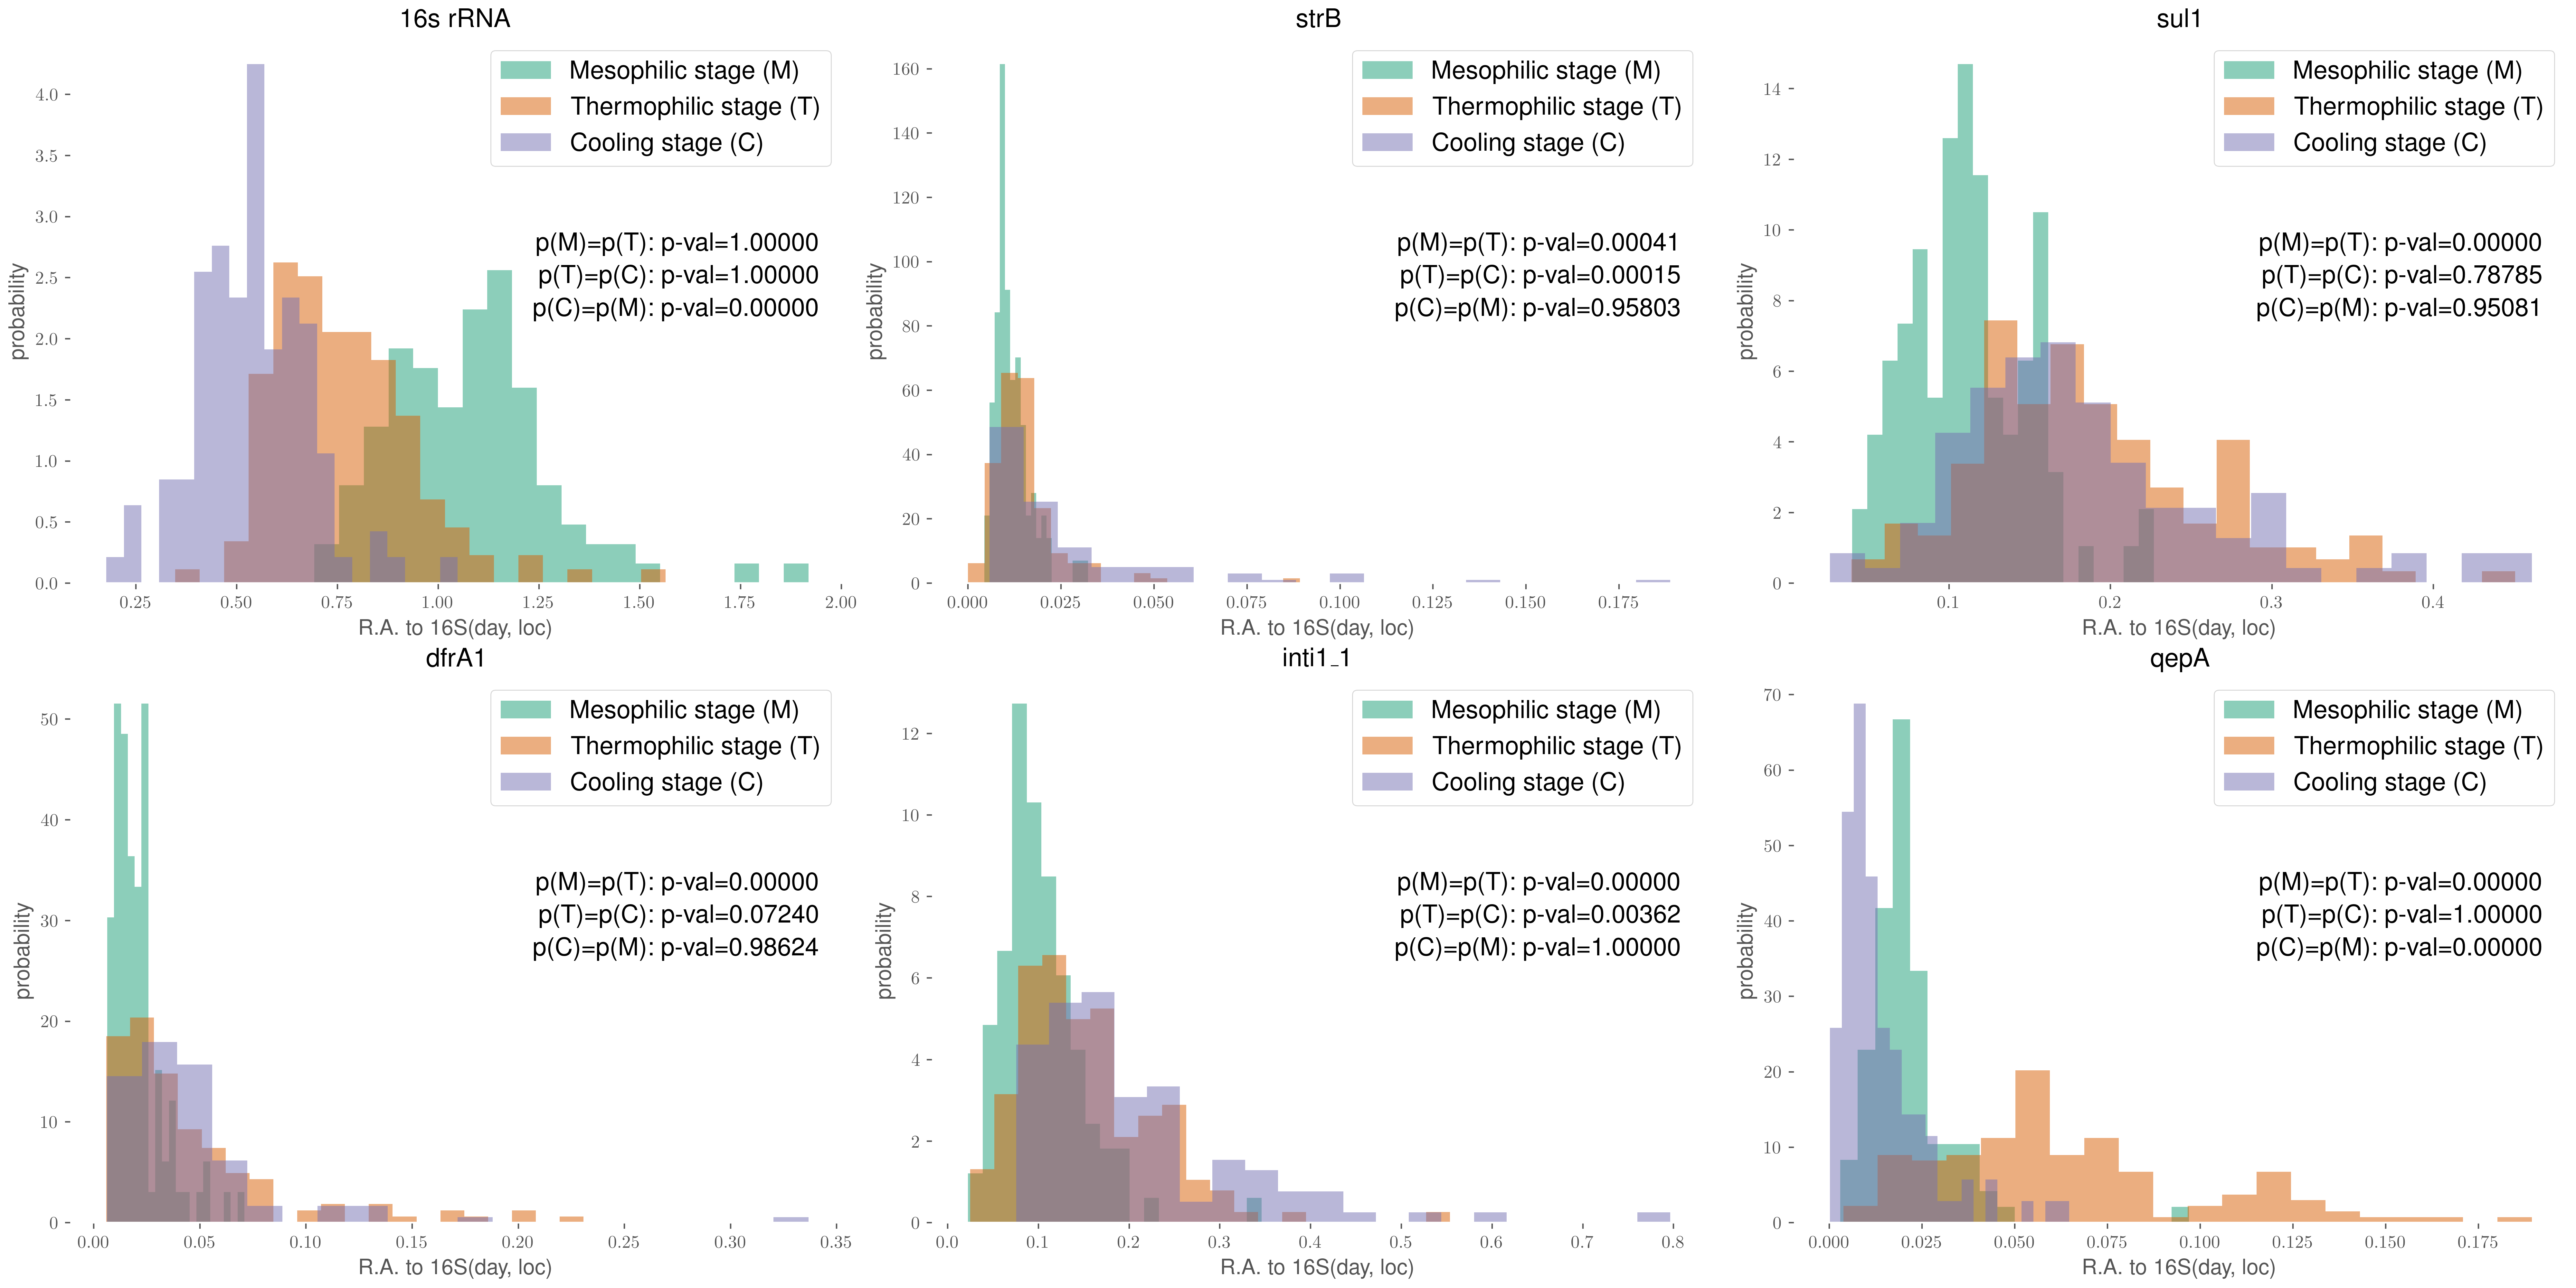
\includegraphics[width=\textwidth]{Figures/Sian_heating_hists_first_6_assays.png}
\end{frame}
\subsection{Temporally resolved data}
\begin{frame}{Relative abundances - updated}
Relative abundances computed using double delta method: temporally linked values, new patterns revealed.
	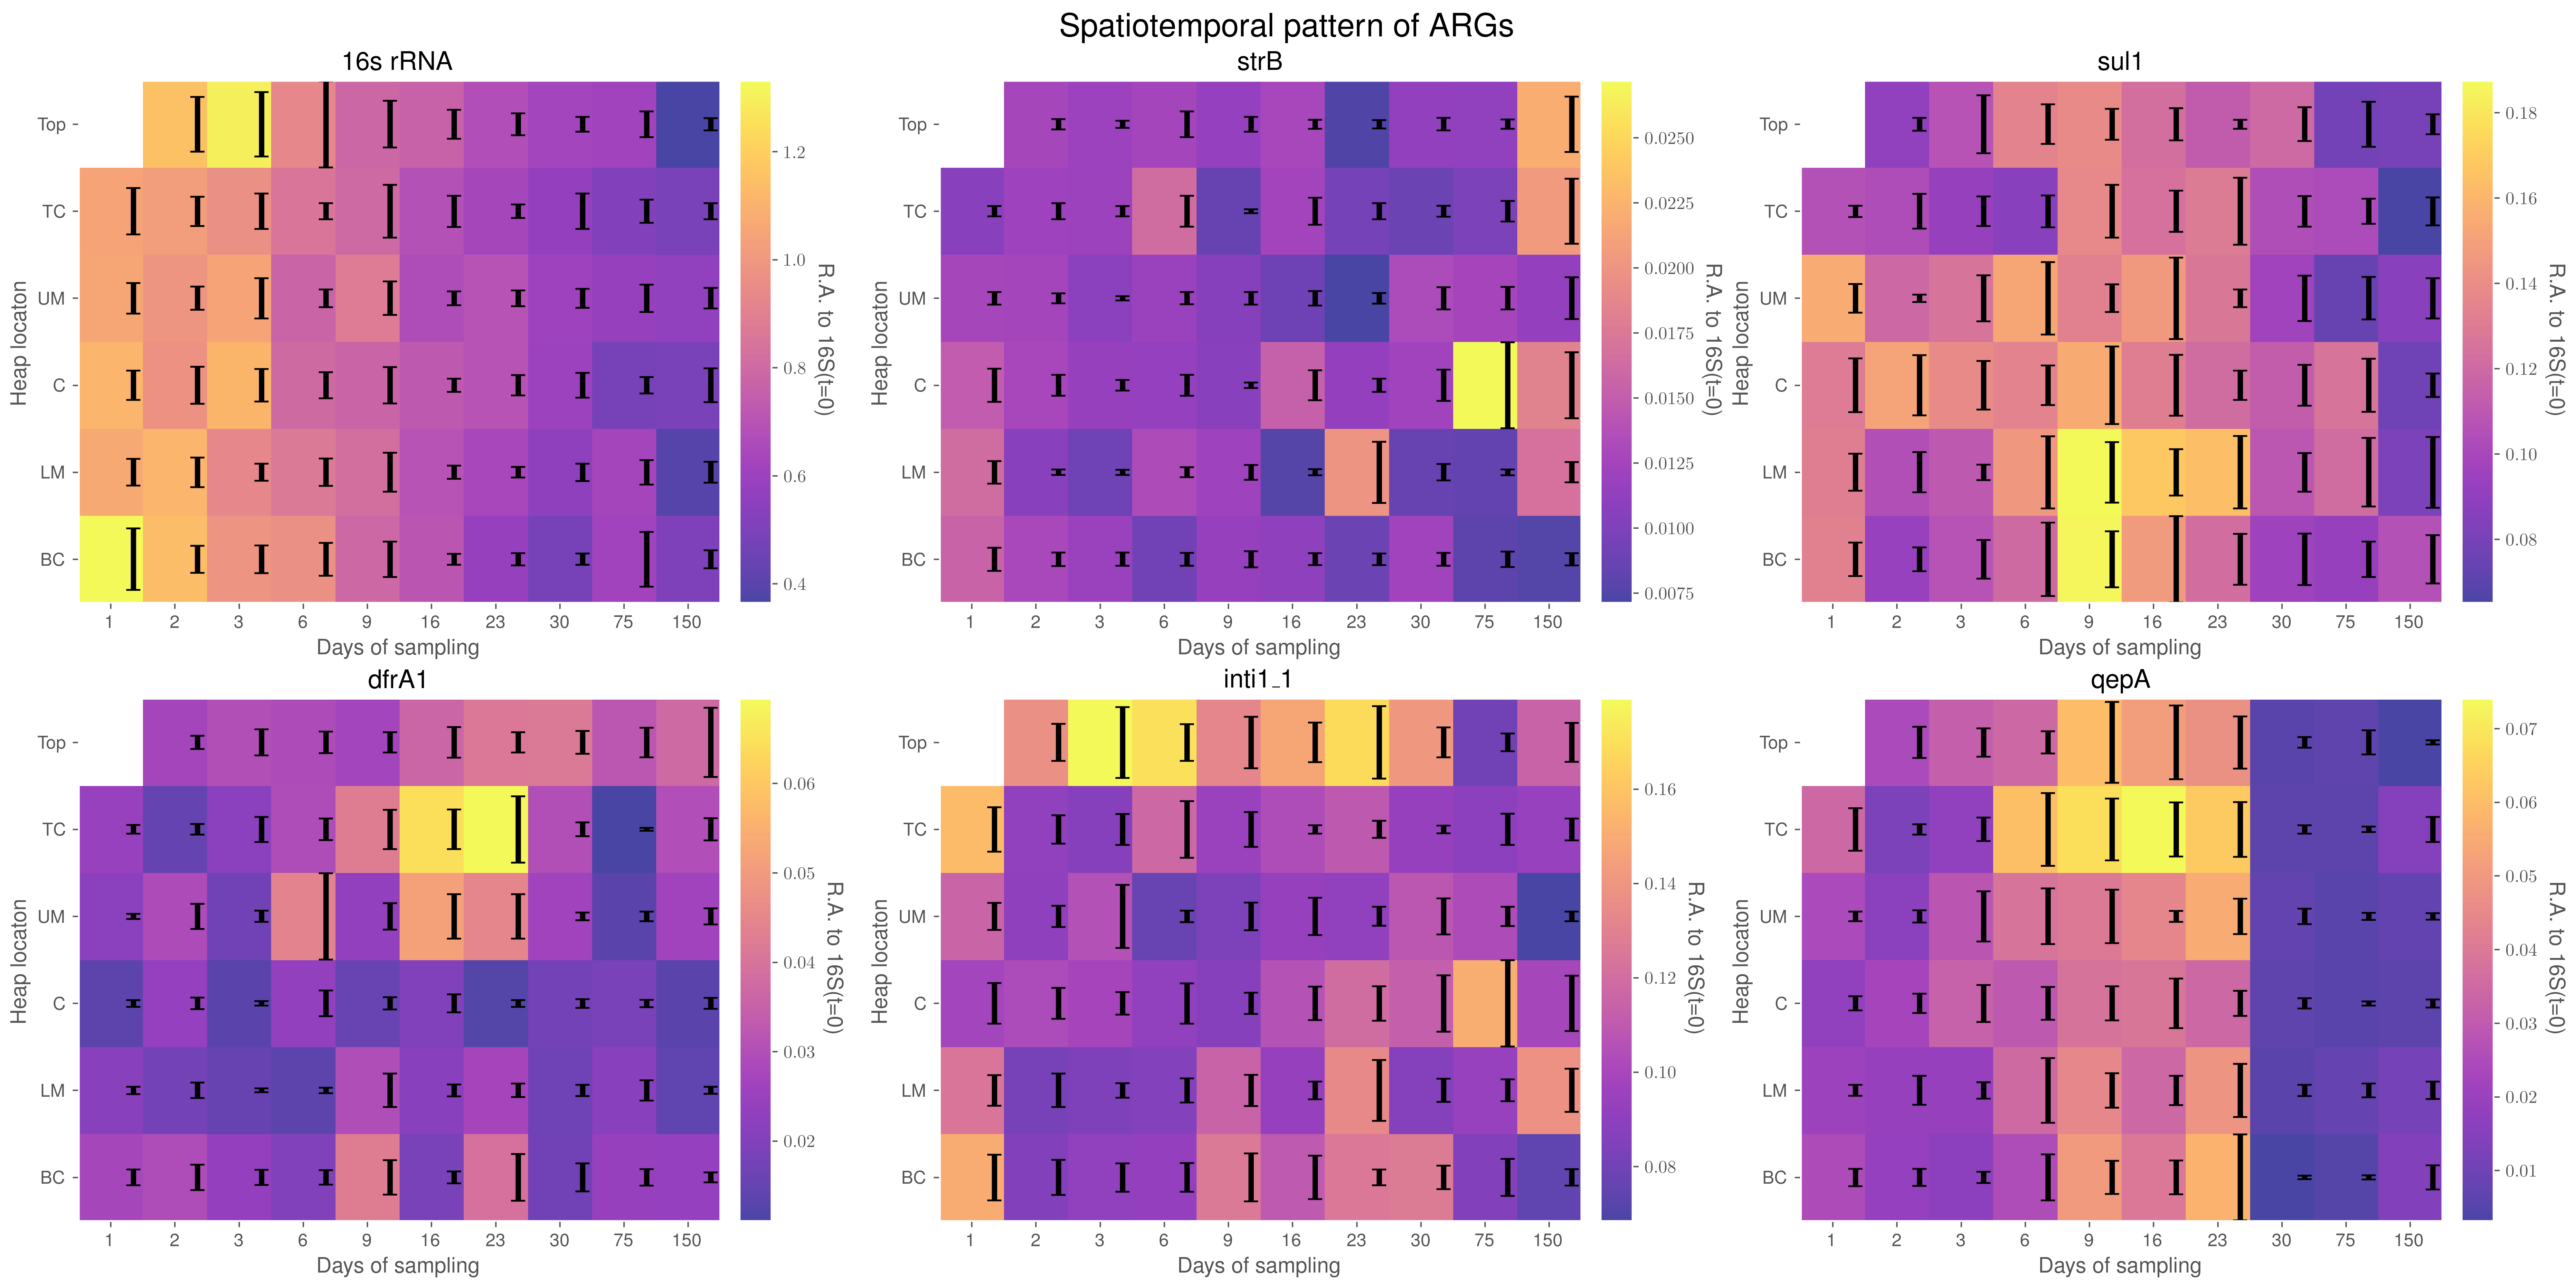
\includegraphics[width=\textwidth]{Figures/Sian_spatial_variation_first6_assays_with_errorbar_day0.png}
\end{frame}
\begin{frame}{Relative abundances - updated}
Relative abundances computed using double delta method:
	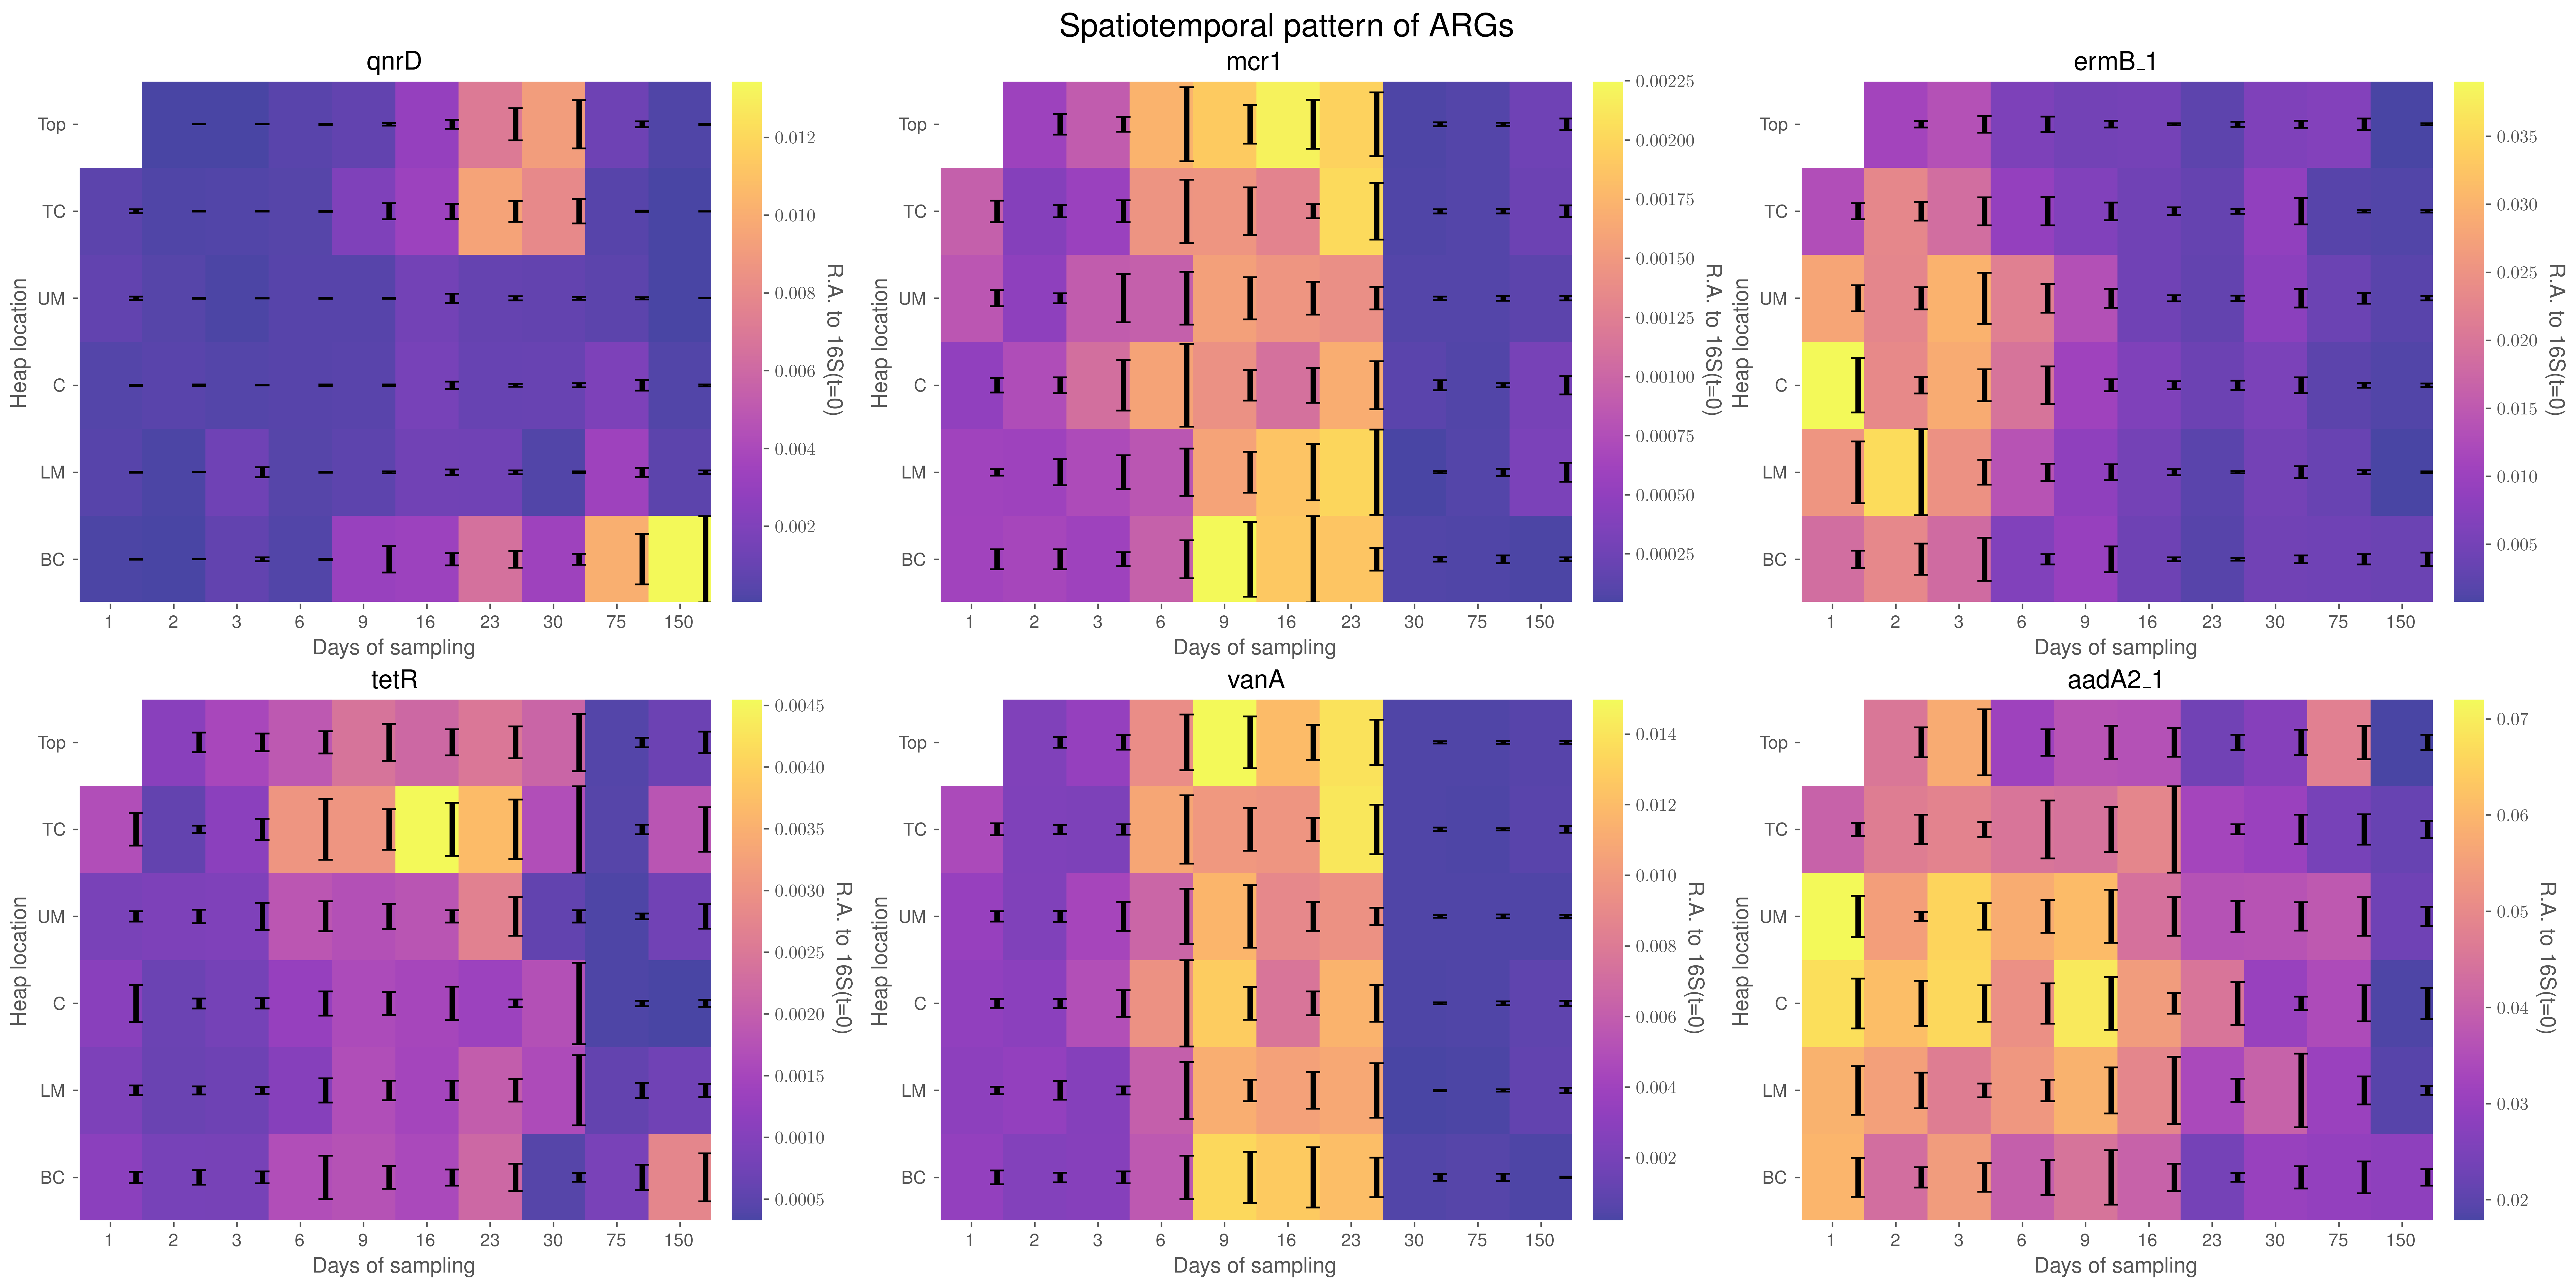
\includegraphics[width=\textwidth]{Figures/Sian_spatial_variation_second6_assays_with_errorbar_day0.png}
\end{frame}
\begin{frame}{Benefit of linking to control sample}
Will validate some patterns:
	\begin{columns}
		\begin{column}{0.5\textwidth}
		\centering
			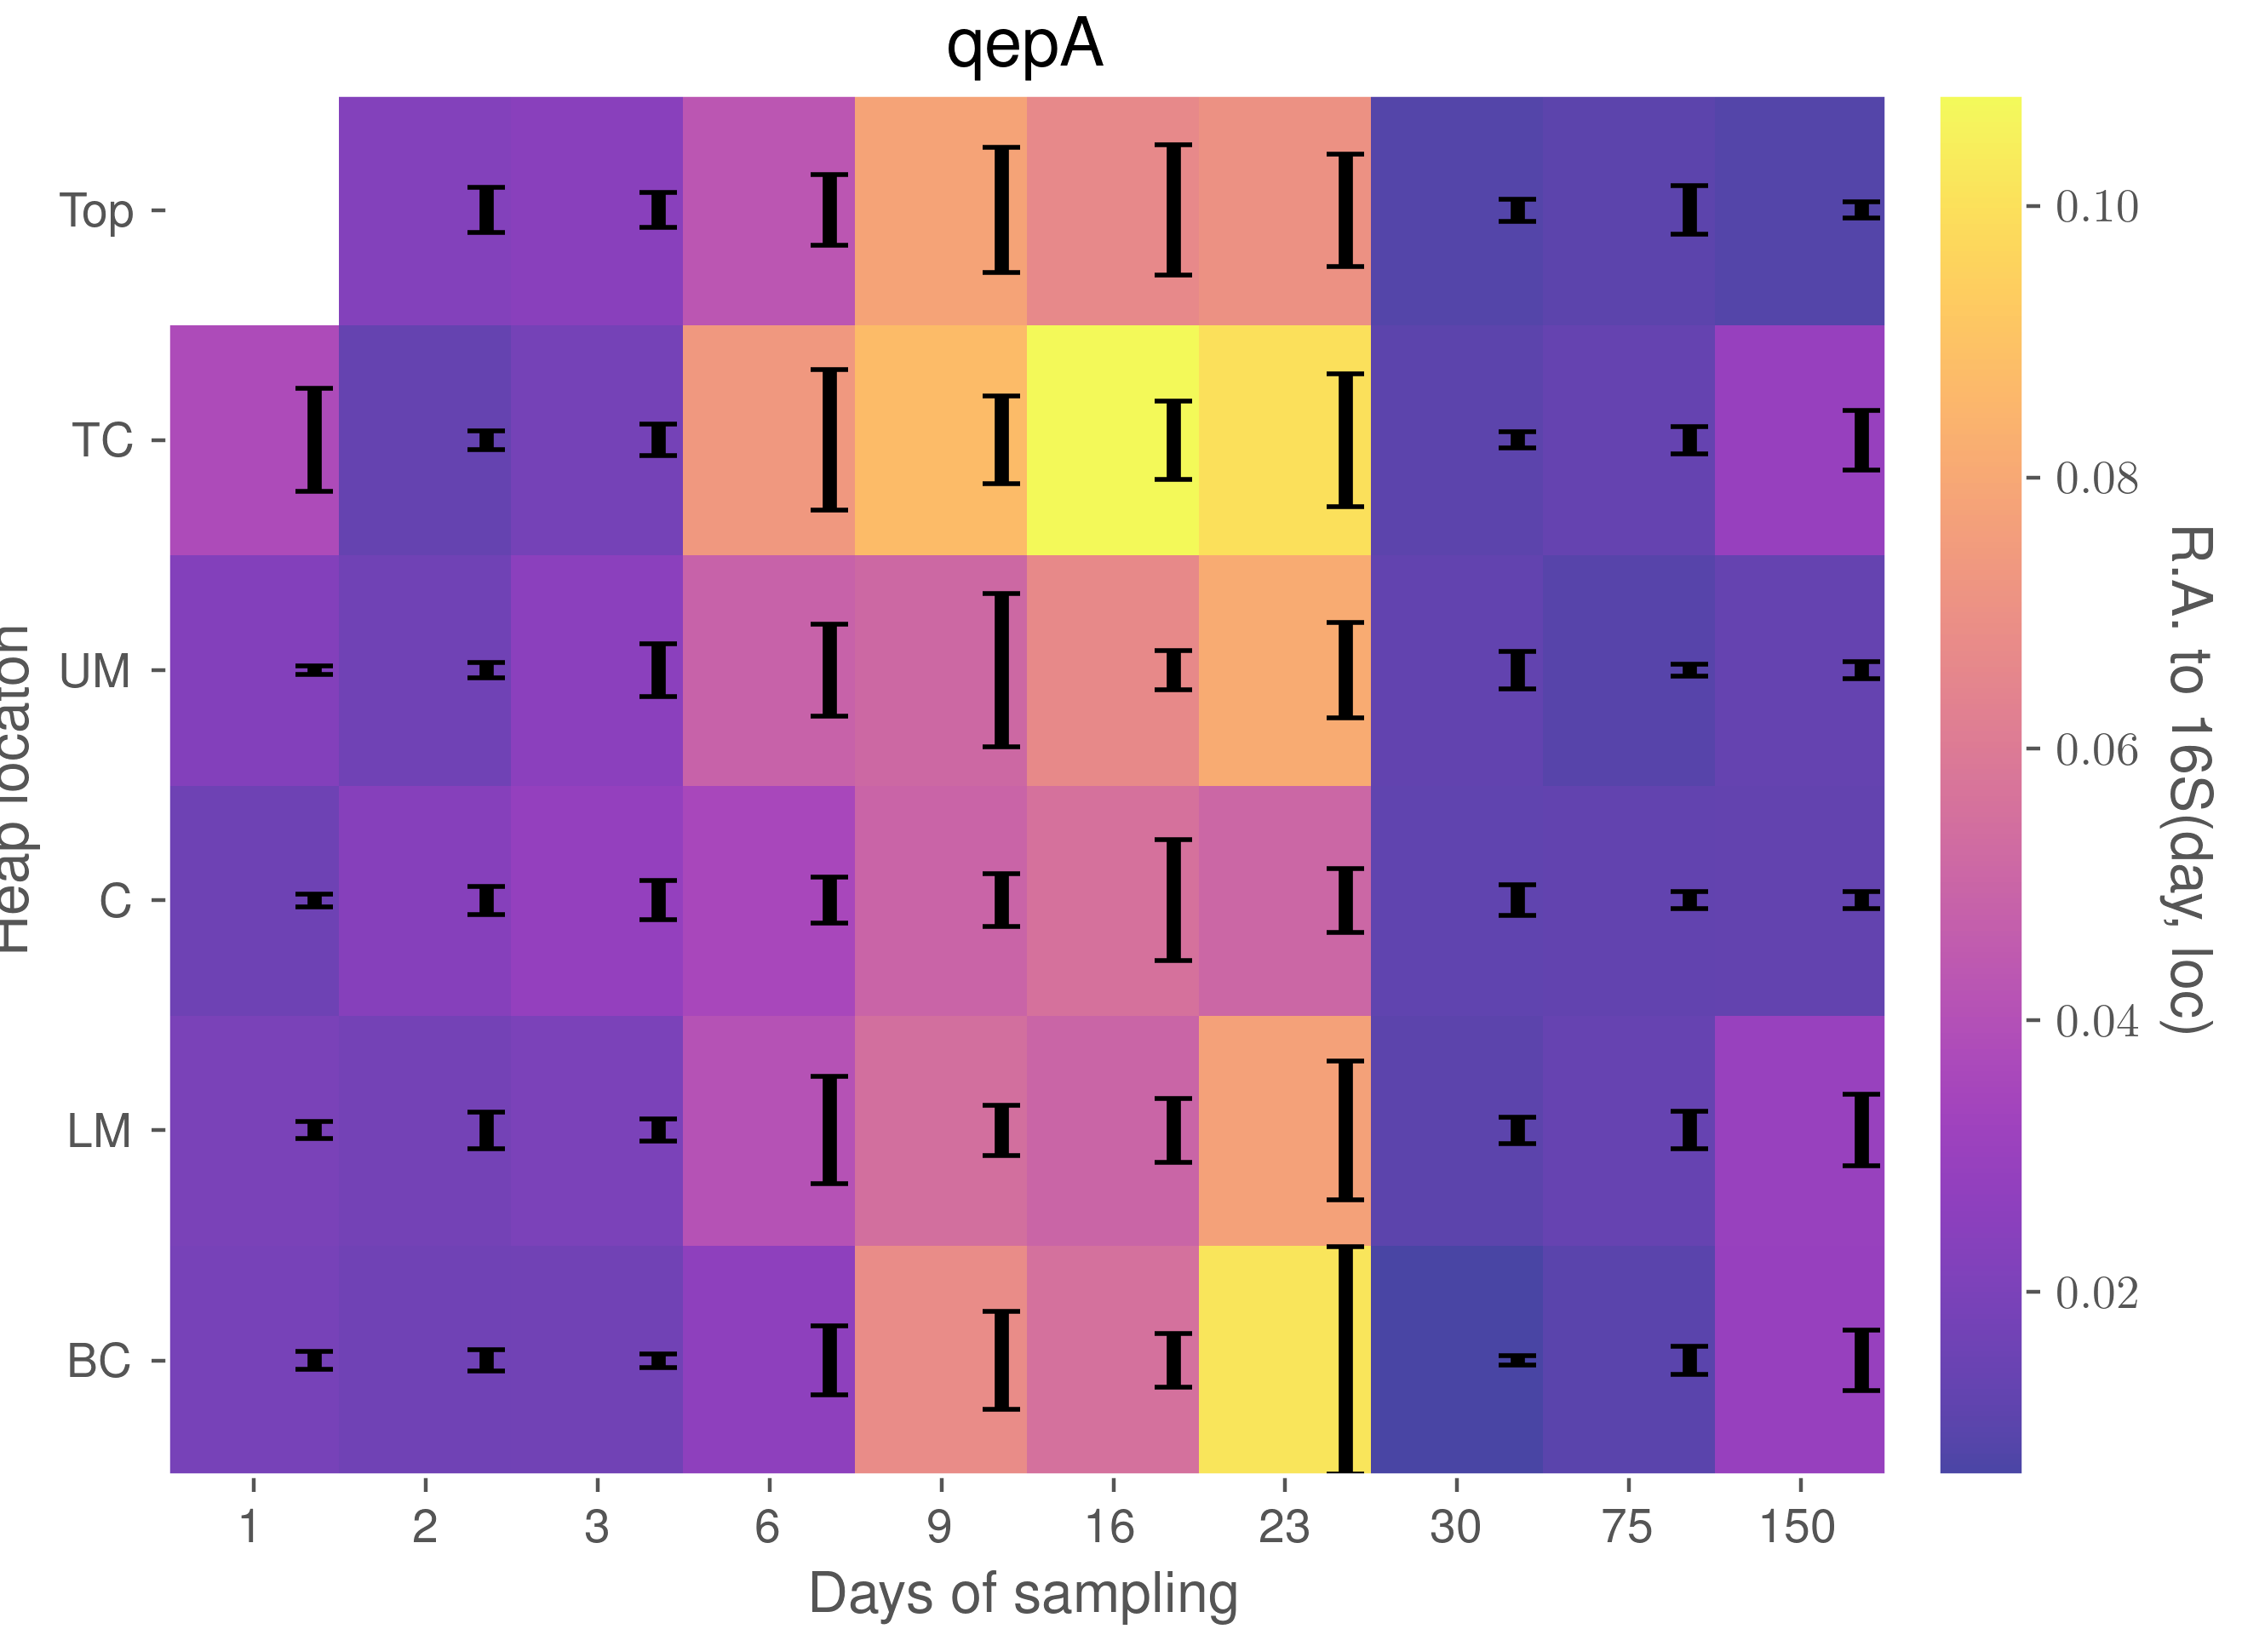
\includegraphics[width=0.7\textwidth]{Figures/same_errorbar.png}
		\end{column}
		\begin{column}{0.5\textwidth}
		\centering
			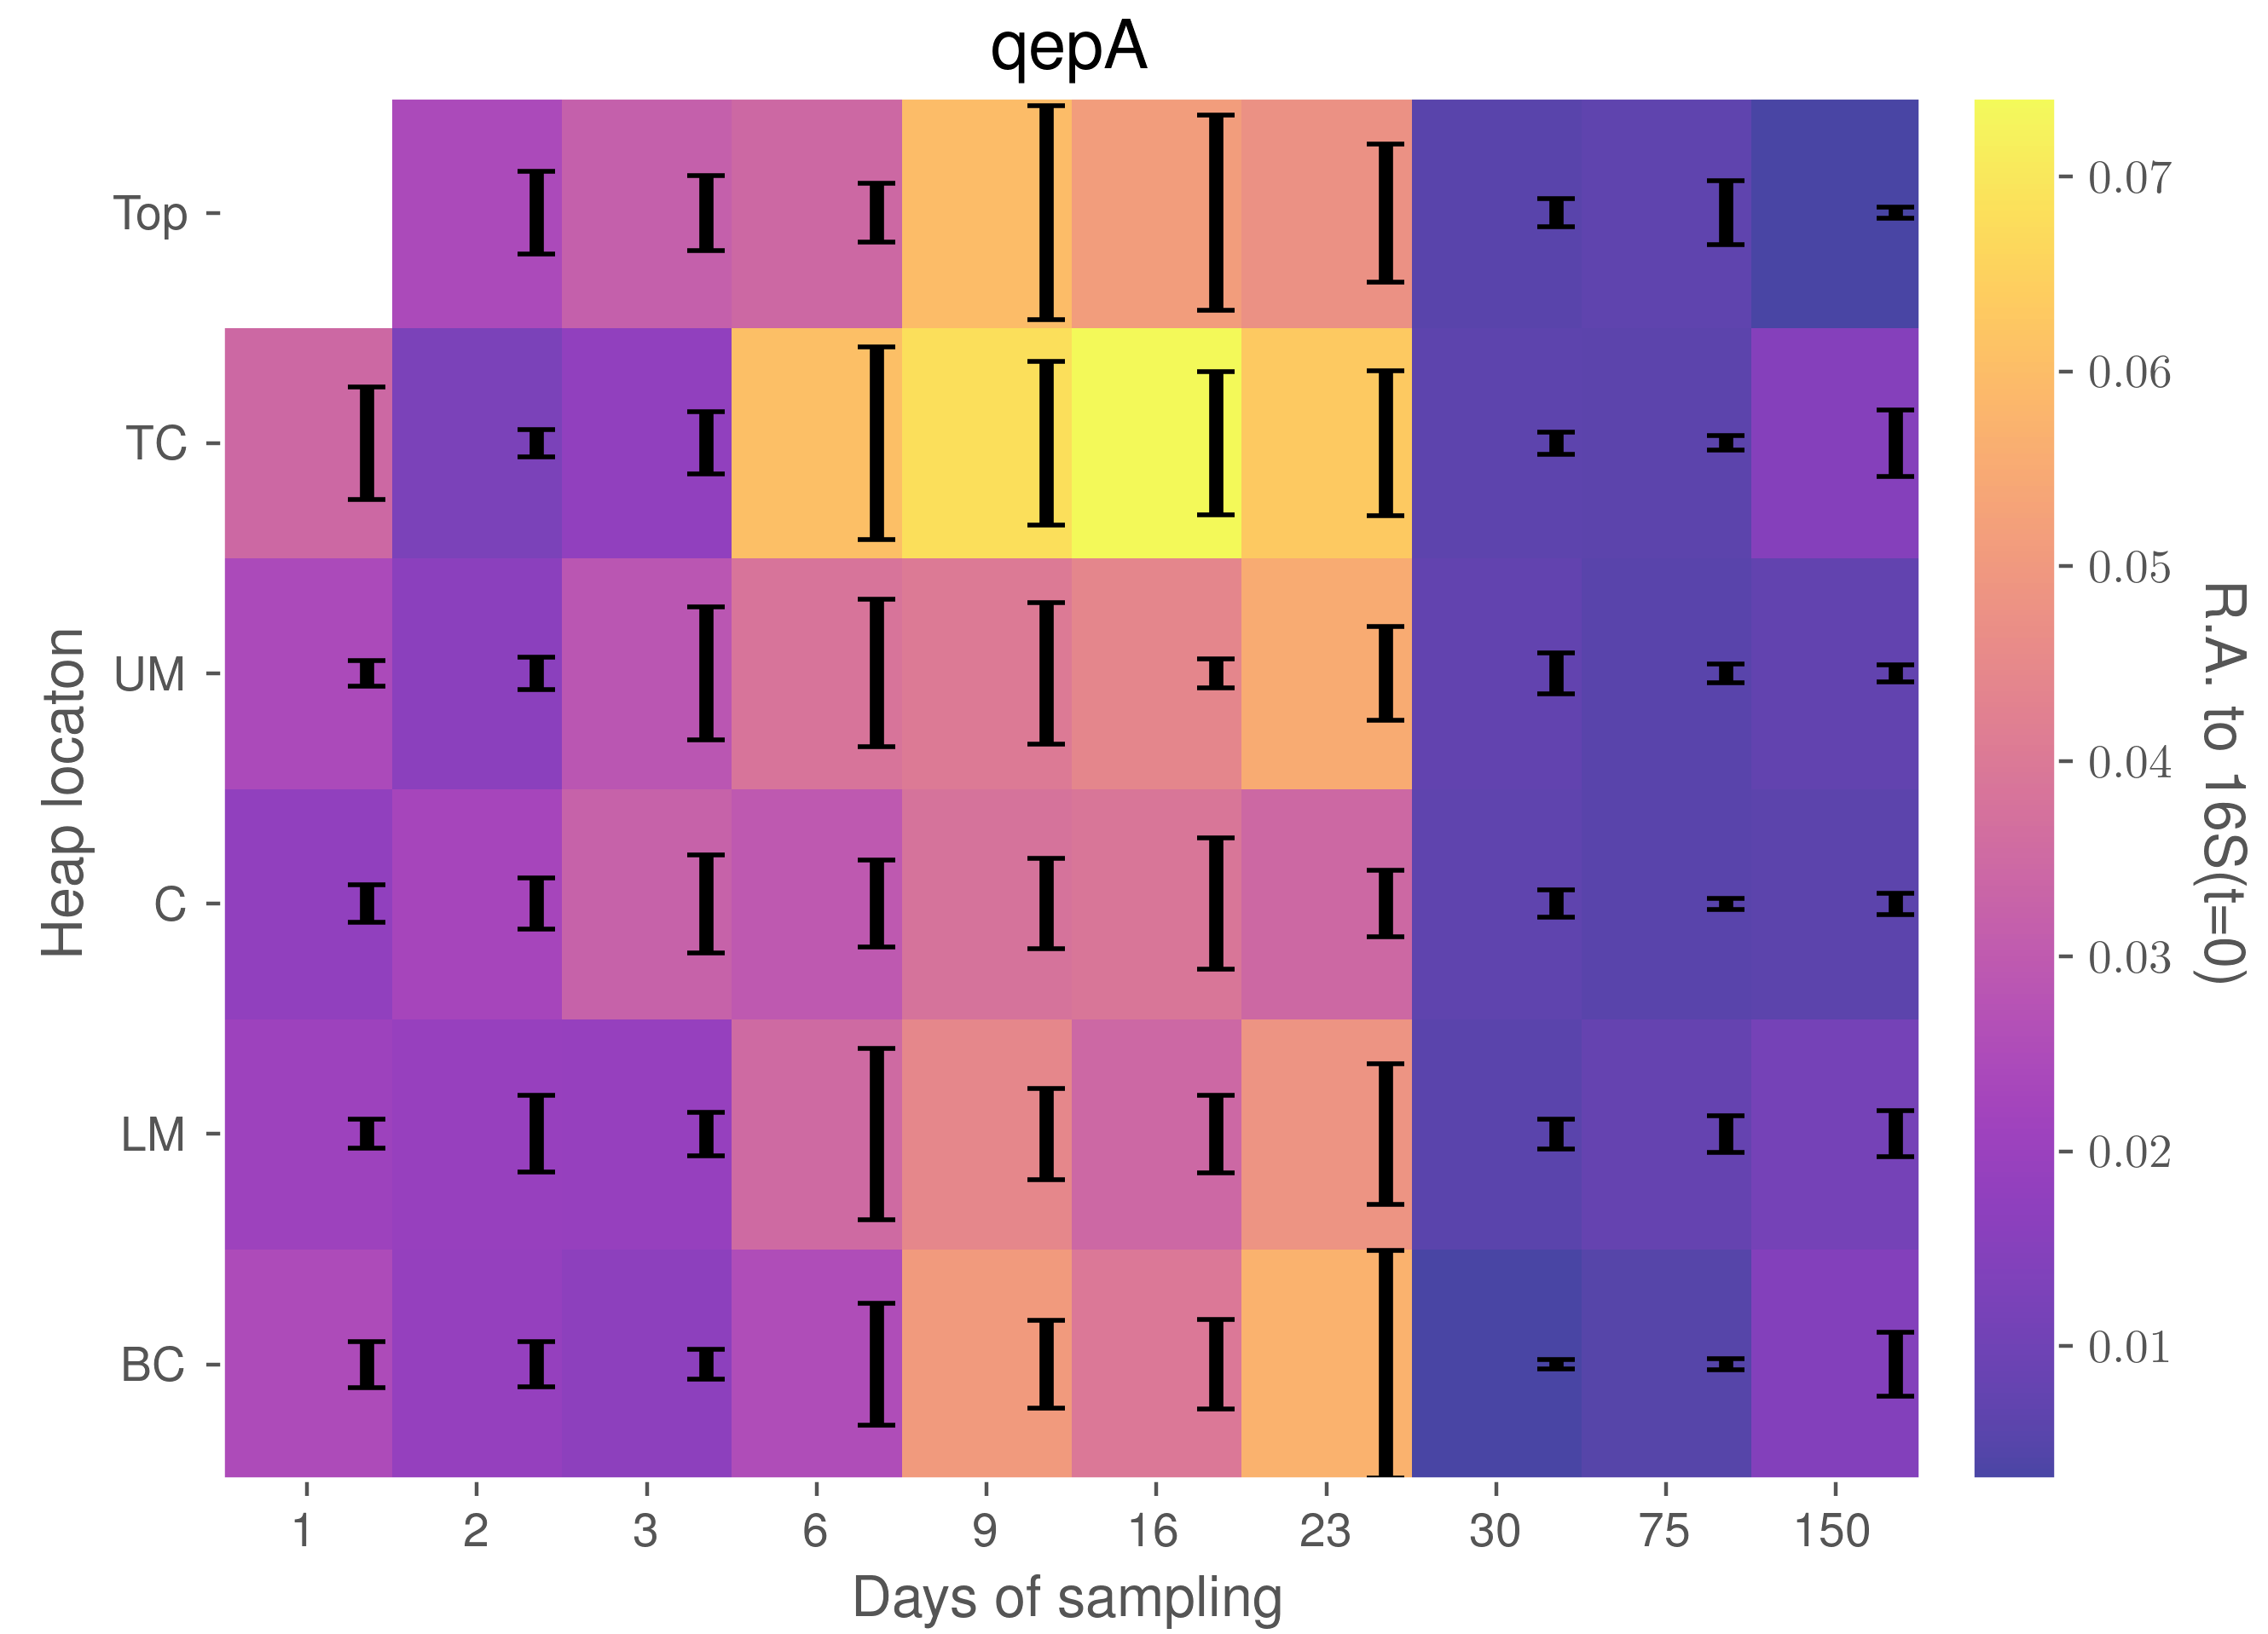
\includegraphics[width=0.7\textwidth]{Figures/same_errorbar_day0.png}
		\end{column}
	\end{columns}
\visible<2->{Or reveal new ones:
	\begin{columns}
			\begin{column}{0.5\textwidth}
			\centering
			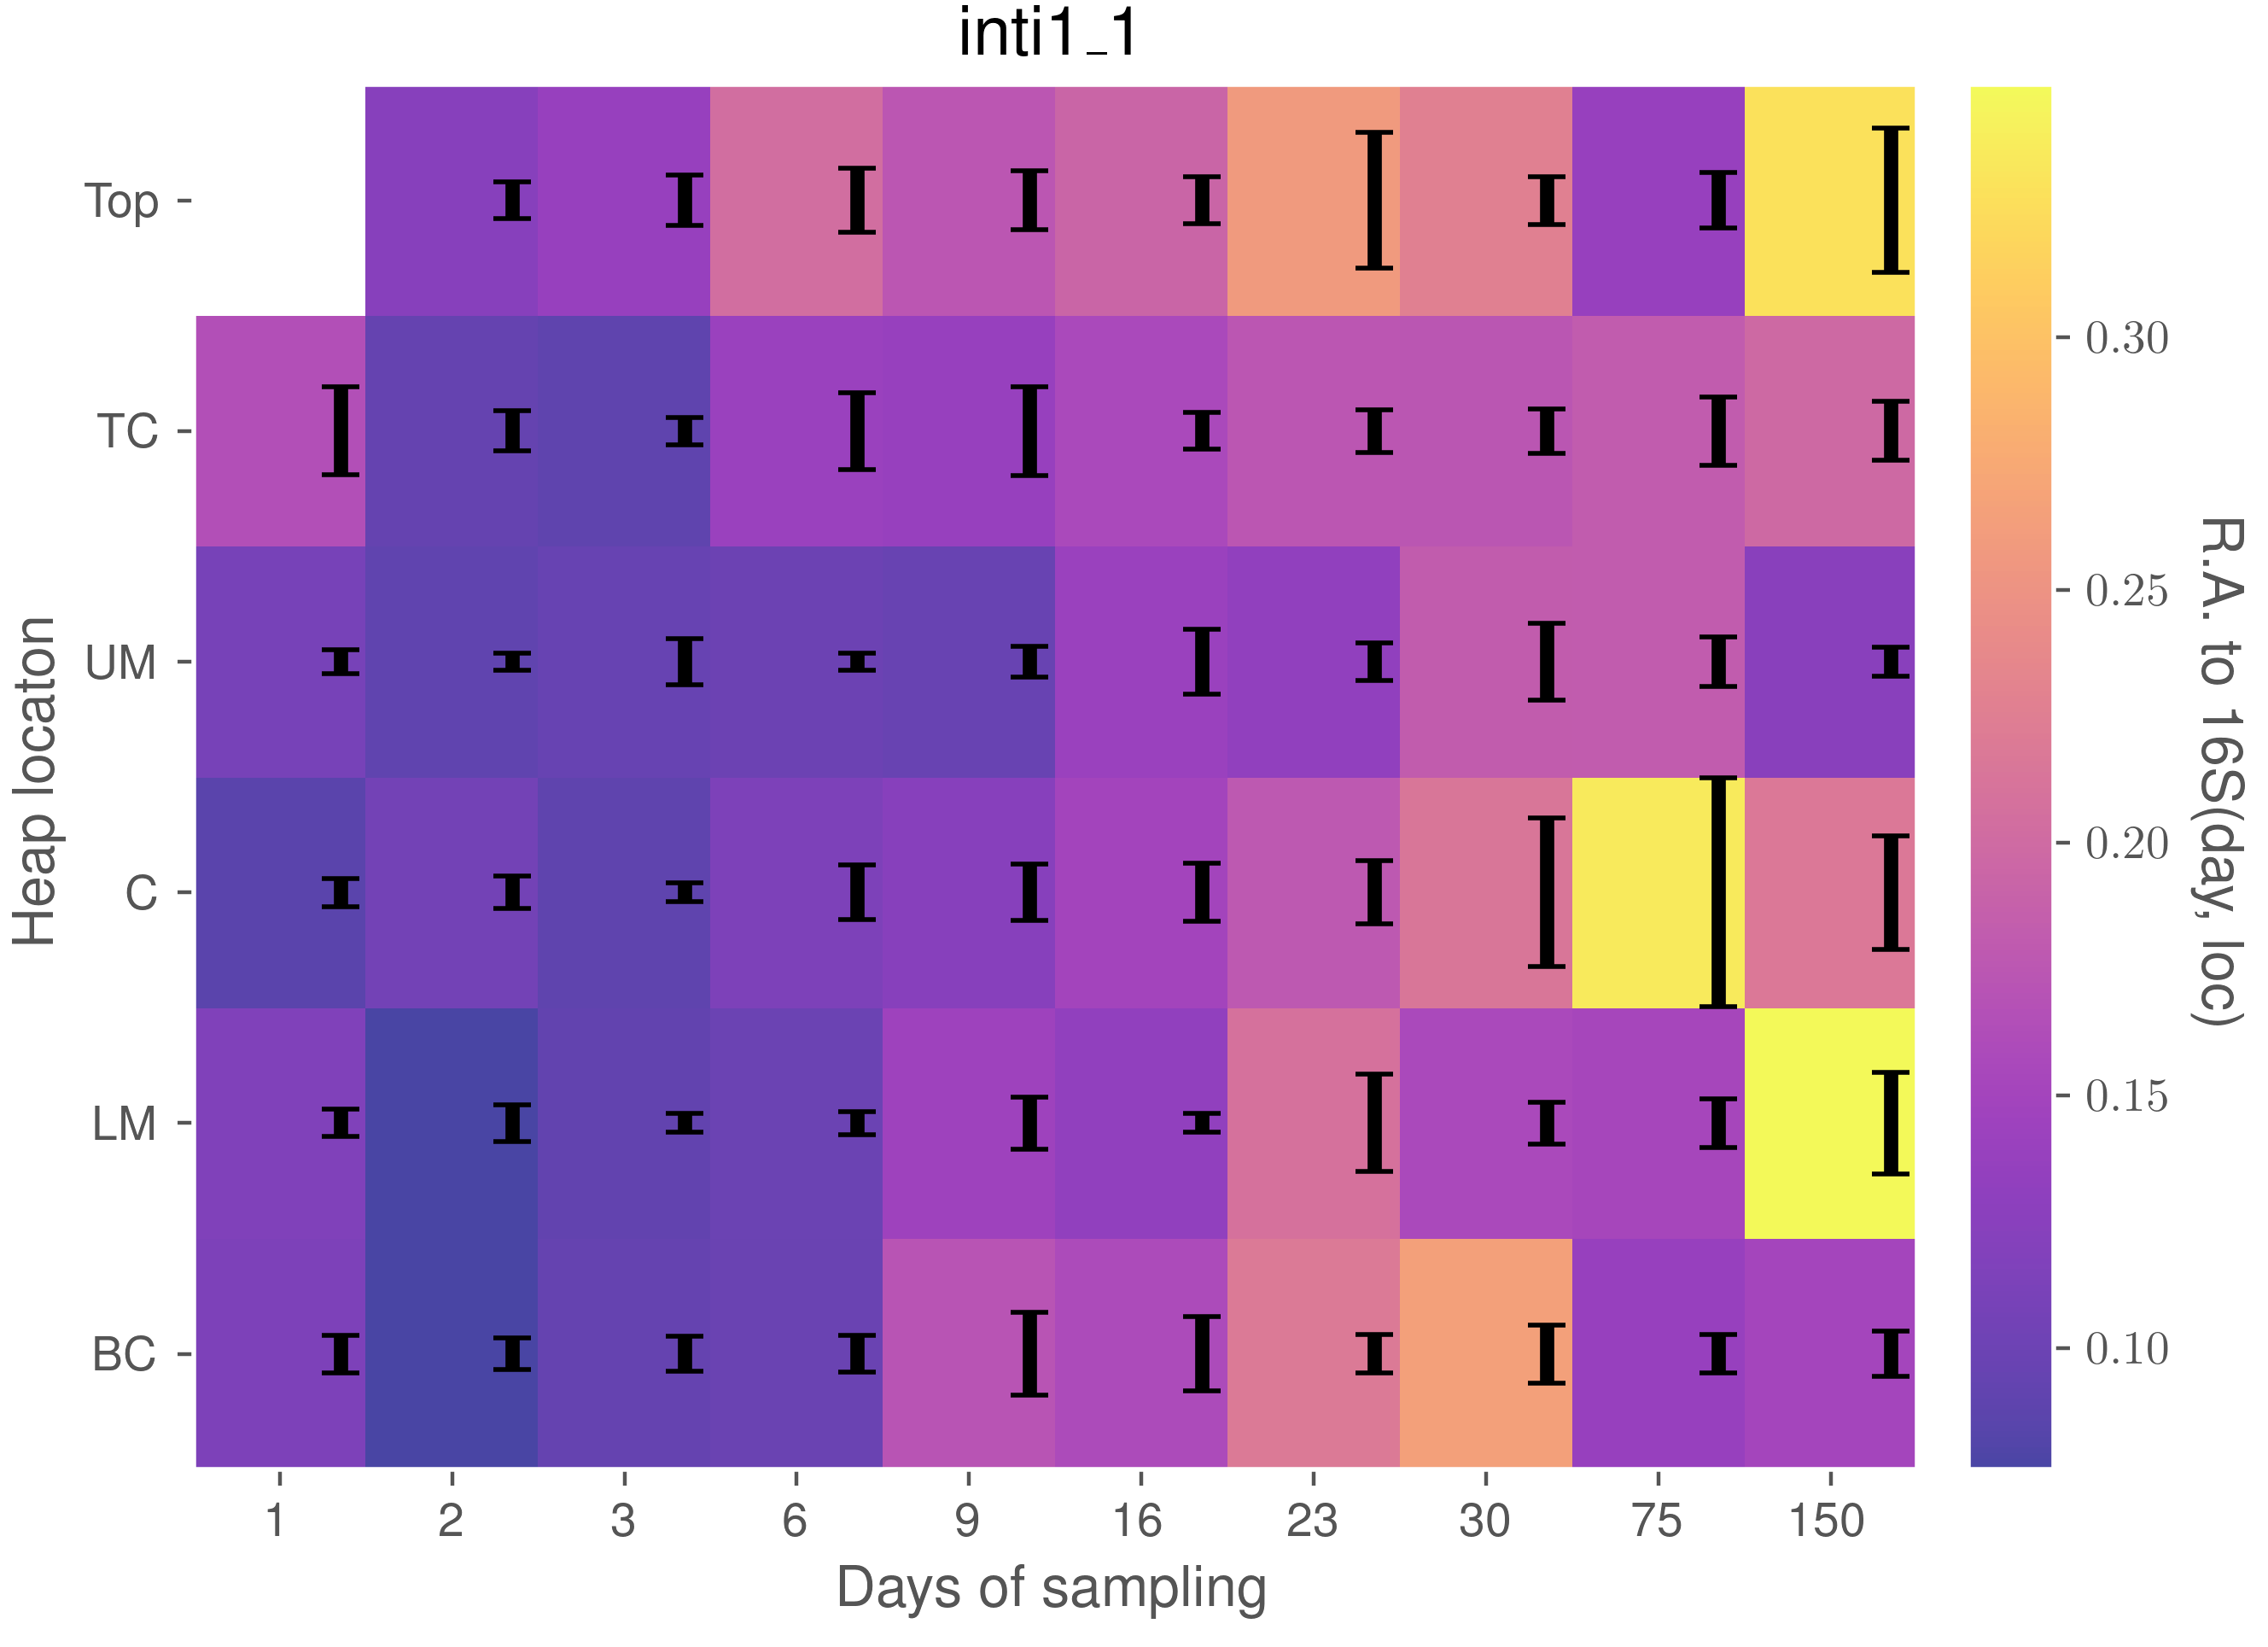
\includegraphics[width=0.7\textwidth]{Figures/changed_errorbar.png}
		\end{column}
		\begin{column}{0.5\textwidth}
		\centering
			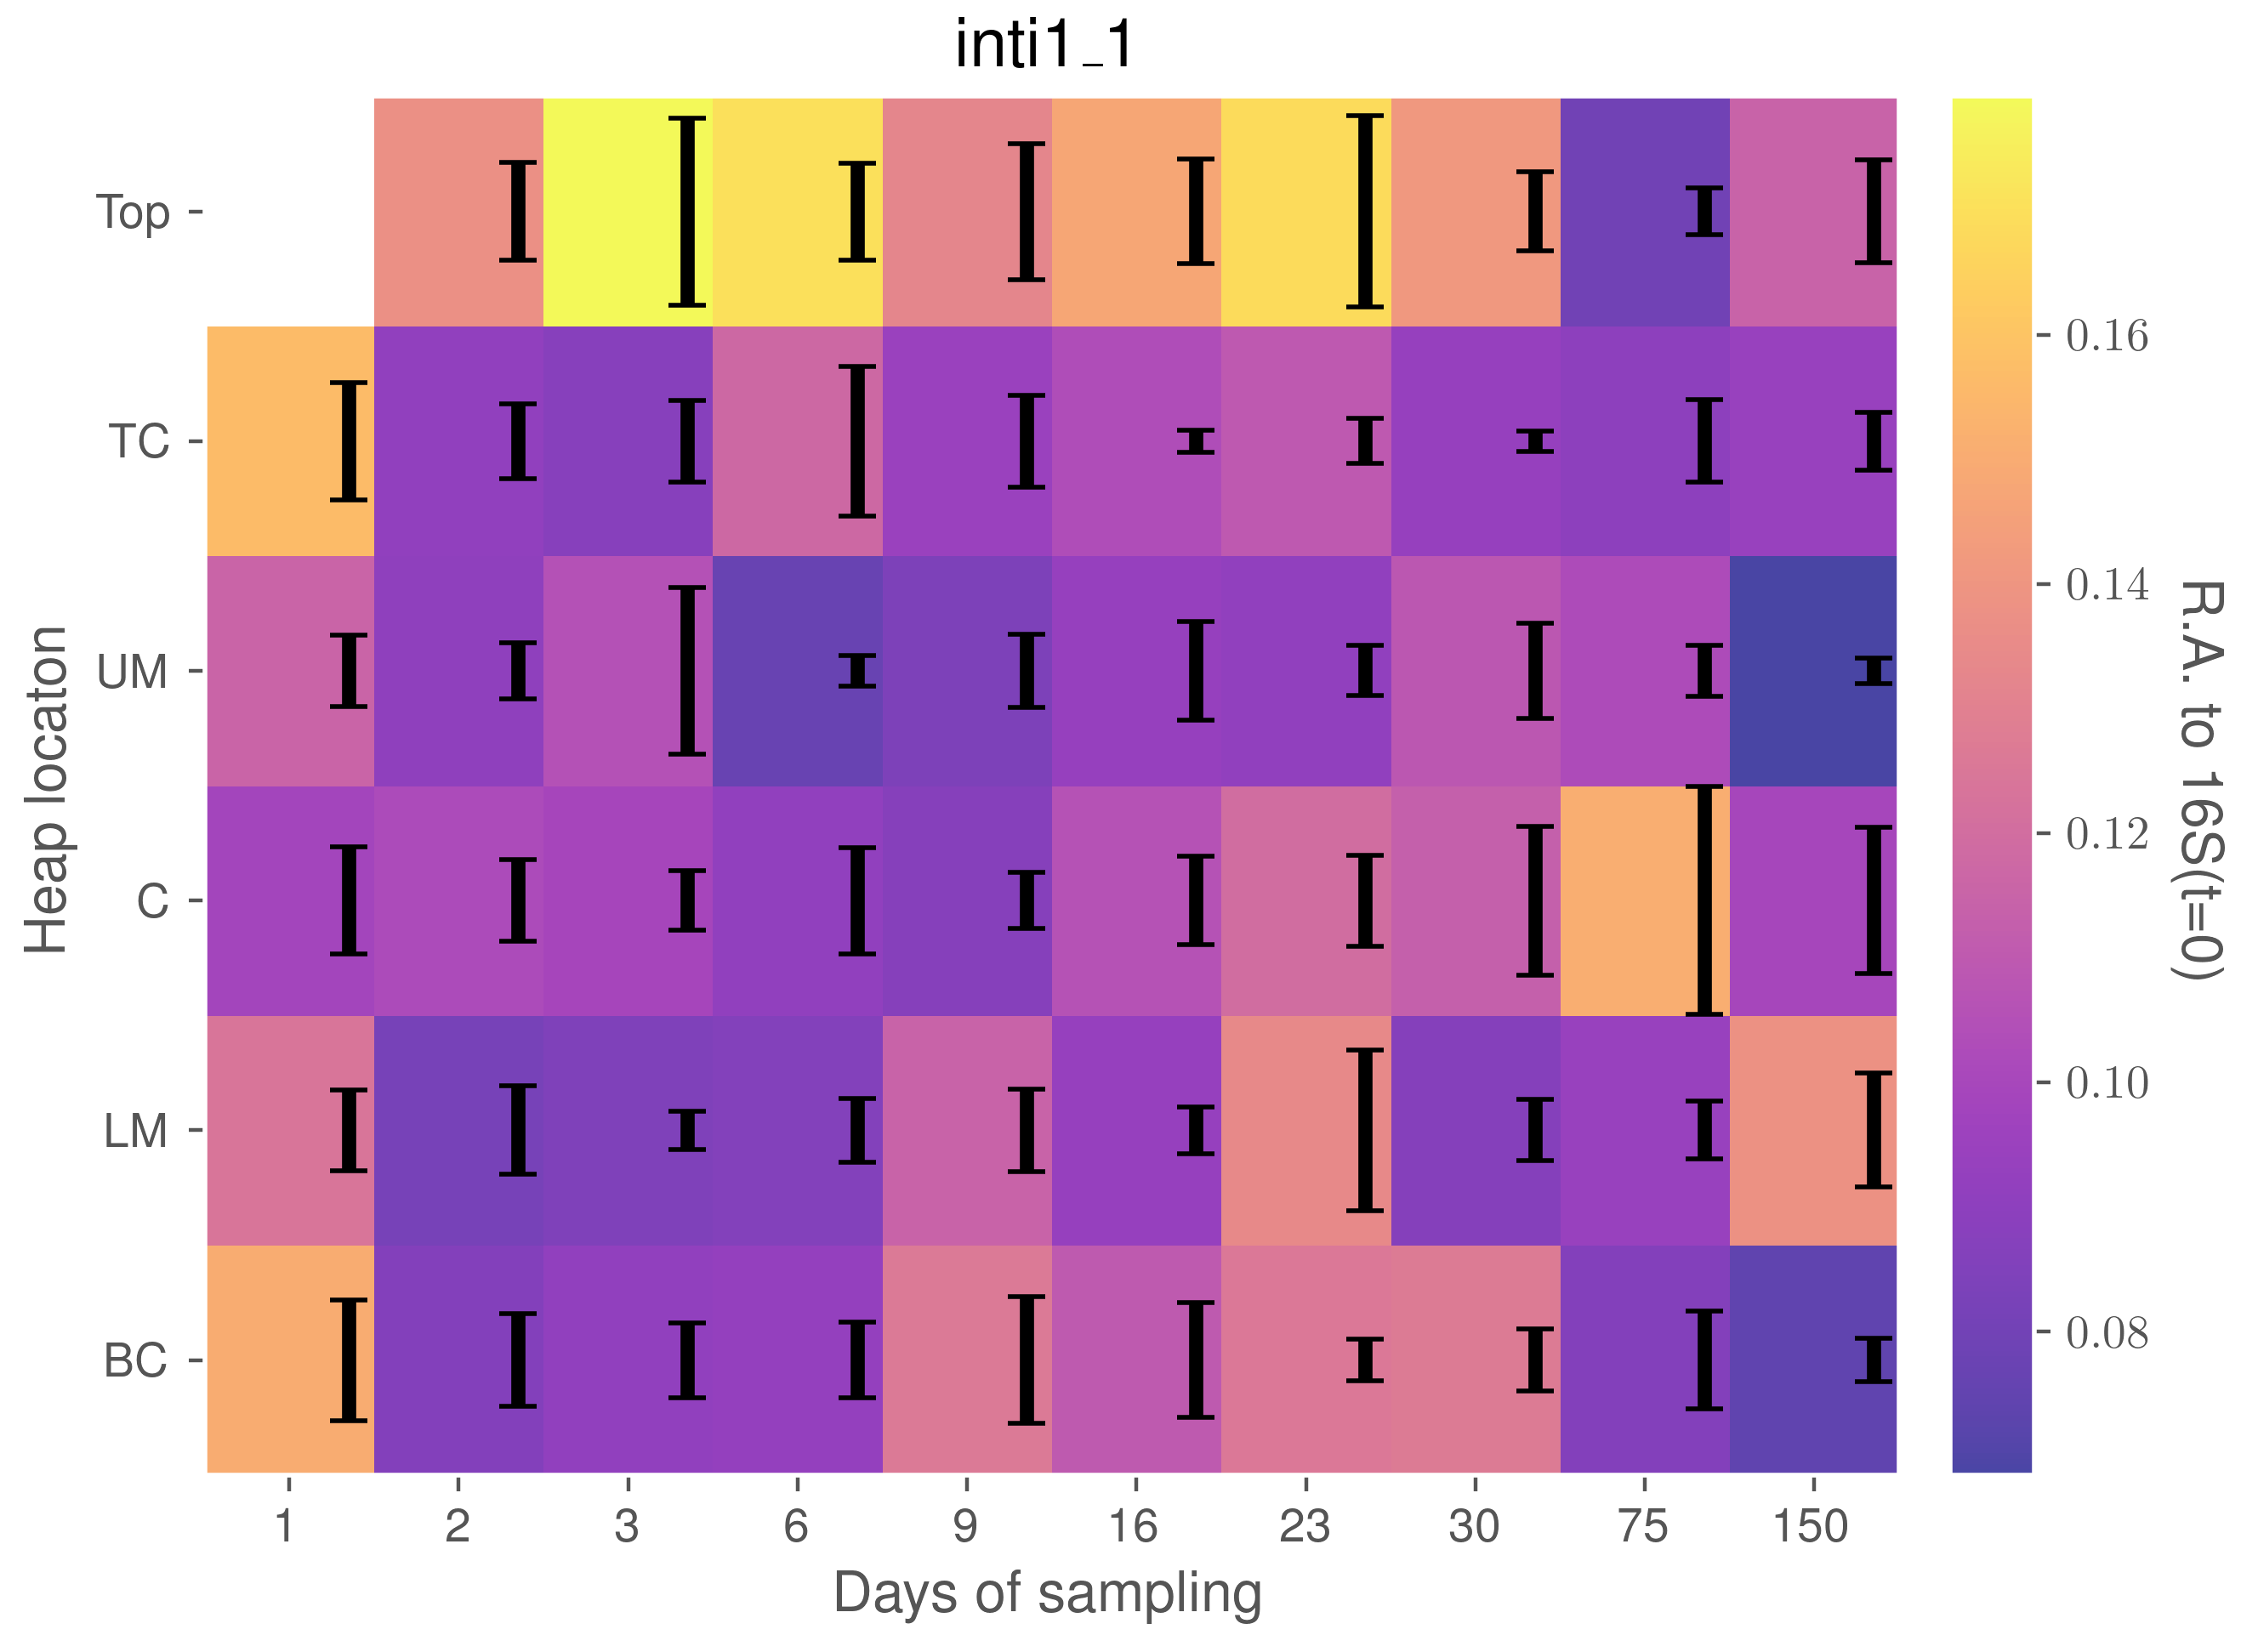
\includegraphics[width=0.7\textwidth]{Figures/changed_errorbar_day0.png}
		\end{column}
	\end{columns}}
\end{frame}
\subsection{Model fitting}
\begin{frame}{Basic principle of model inference}
\begin{columns}
			\begin{column}{0.5\textwidth}
			\centering
			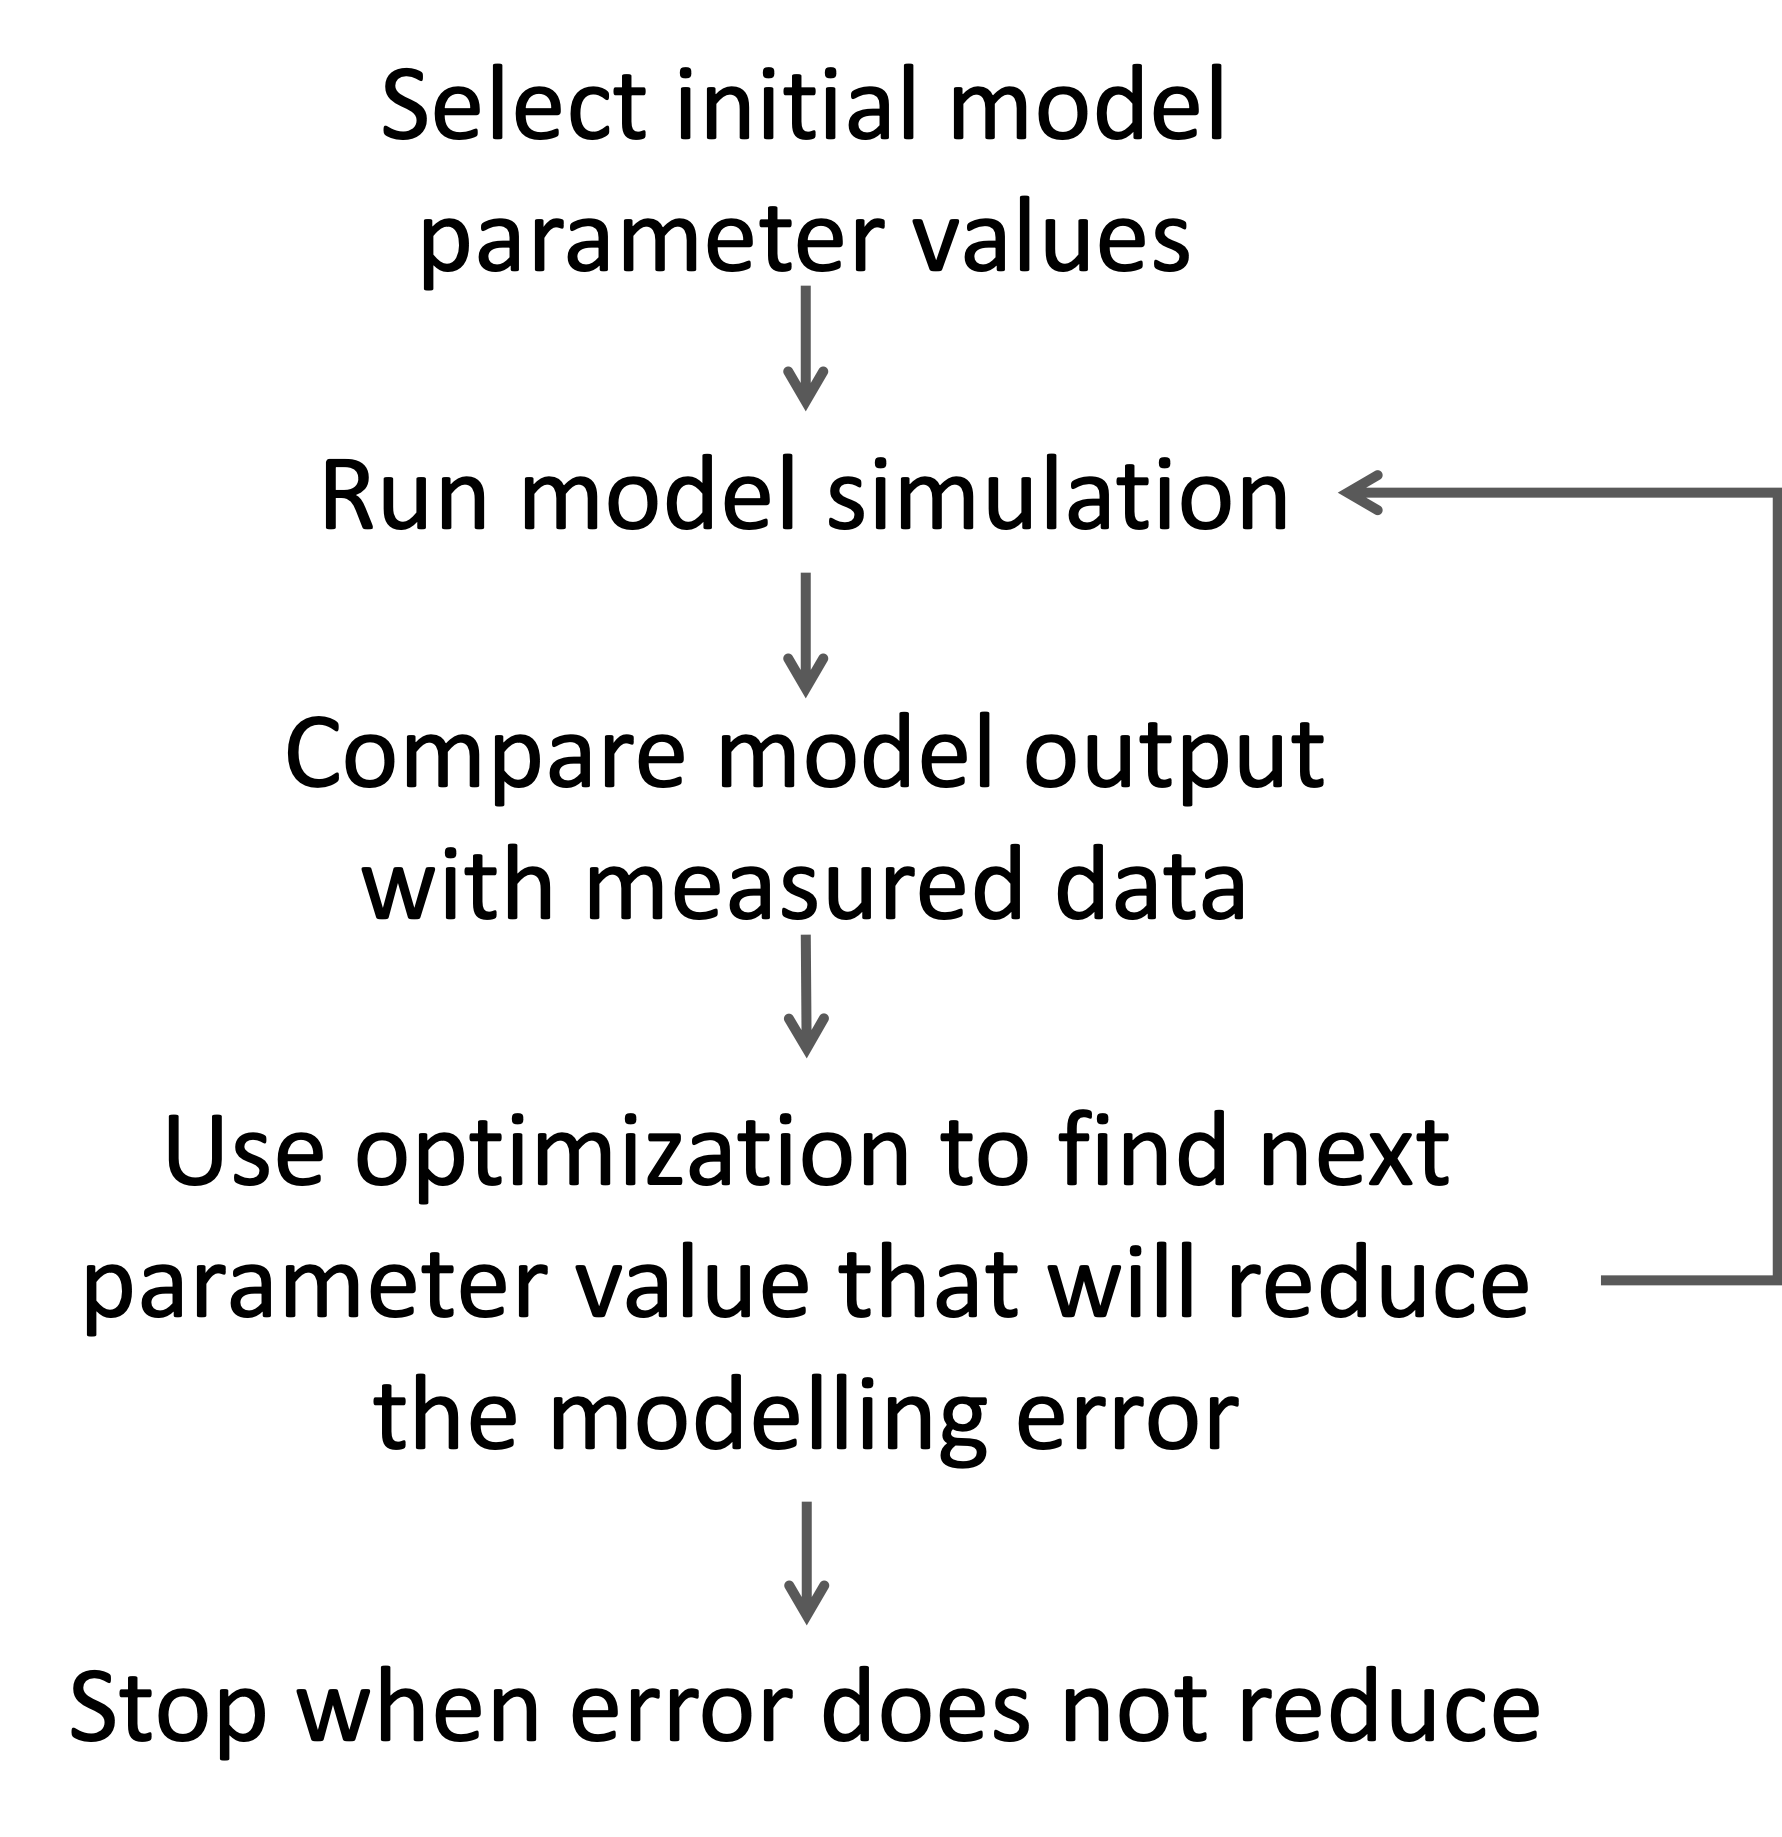
\includegraphics[width=\textwidth]{Figures/inference.png}
		\end{column}
		\begin{column}{0.5\textwidth}
		\centering
			\only<2->{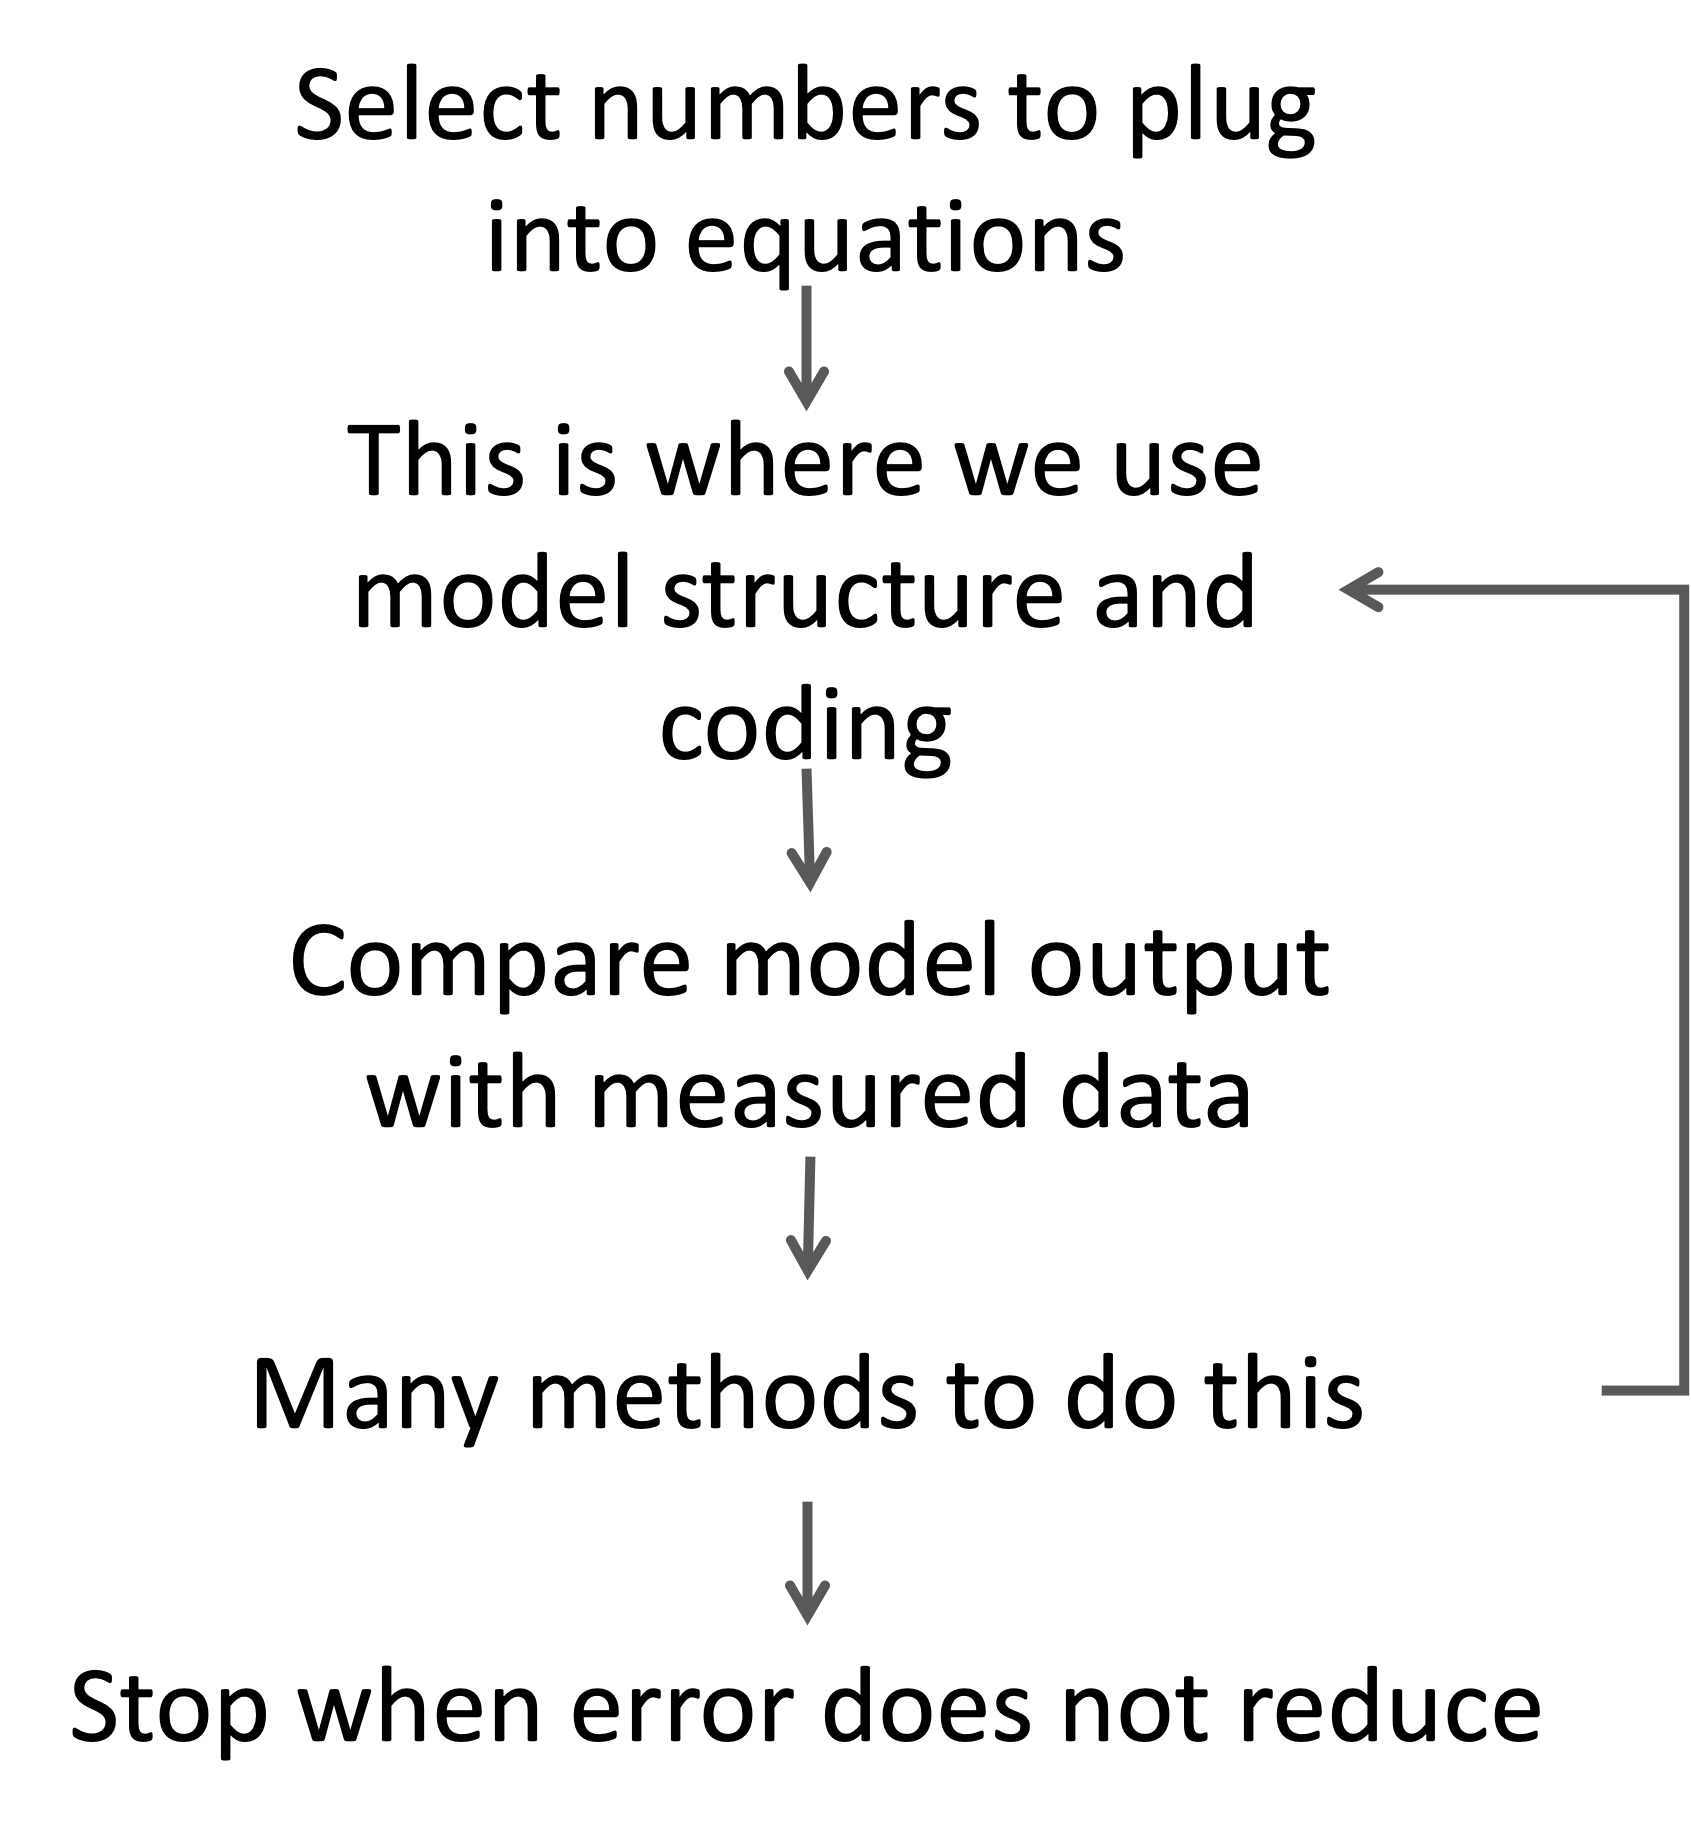
\includegraphics[width=\textwidth]{Figures/inference_laymen.png}}
		\end{column}
	\end{columns}
\end{frame}
\begin{frame}{Relaxing defining assumptions of our model}
	\begin{itemize}
		\item No taxonomic information available, modelling functional subpopulations instead.
		\item PDE model simulates absolute counts, we implement an additional model of the measurement process to compare RAs with RAs.
		\item 16S - total population (everything that is alive).
		\item No co-resistances to multiple drugs
		\item Add ARG RAs together and substract from 16S to obtain \textbf{sensitive} subpopulation.
		\item Fitting to data up to hr 500 - mesophilic and thermophilic stages only.
	\end{itemize}
\end{frame}
\begin{frame}{Identifiability issues}
	\begin{itemize}
		\item Cannot use ComBase!
		\item $\mathrm{T}_{min}, \mathrm{T}_{max}, \mathrm{T}_{opt}$ , $\mathrm{pH}_{min}, \mathrm{pH}_{max}, \mathrm{pH}_{opt}$, $a_{w0}$ become unknown parameters for each subpopulation.
		\item Replace limiting factors of growth rates by Gaussian curves, reduce the number of unknown parameters to $\mu(\mathrm{T}), \sigma(\mathrm{T}), \mu(\mathrm{pH}), \sigma(\mathrm{pH}), a_{w0}$. 
		\item Only include 4 ARGs that have "noticeable" pattern + sensitive population
		\item Horizontal gene transfer becomes a confounding factor.
		\item Total number of unknown model parameters: 3 + 5*(3 + 5) = 43.
	\end{itemize}
\end{frame}
\begin{frame}{Some implementation details}
\begin{itemize}
	\item We are fitting model to temperature and ARG data - multi-objective optimisation
	\item Way more data points for temperature then for ARGs - normalise the errors by numbers of datapoints
	\item Weighs must be assigned to each modelling error to ensure that fitting incorporates all information equally.
	\item CMA-ES - "speedy" population based optimisation method from evolutionary strategies (ES).
	\item Constrain all parameters to be > 0 - physically meaningful.
	\item Run for 1500 generations.
\end{itemize}	
\end{frame}
\subsection{Fitting results}
\begin{frame}{Example of parameter evolution in CMA-ES}
	\centering
	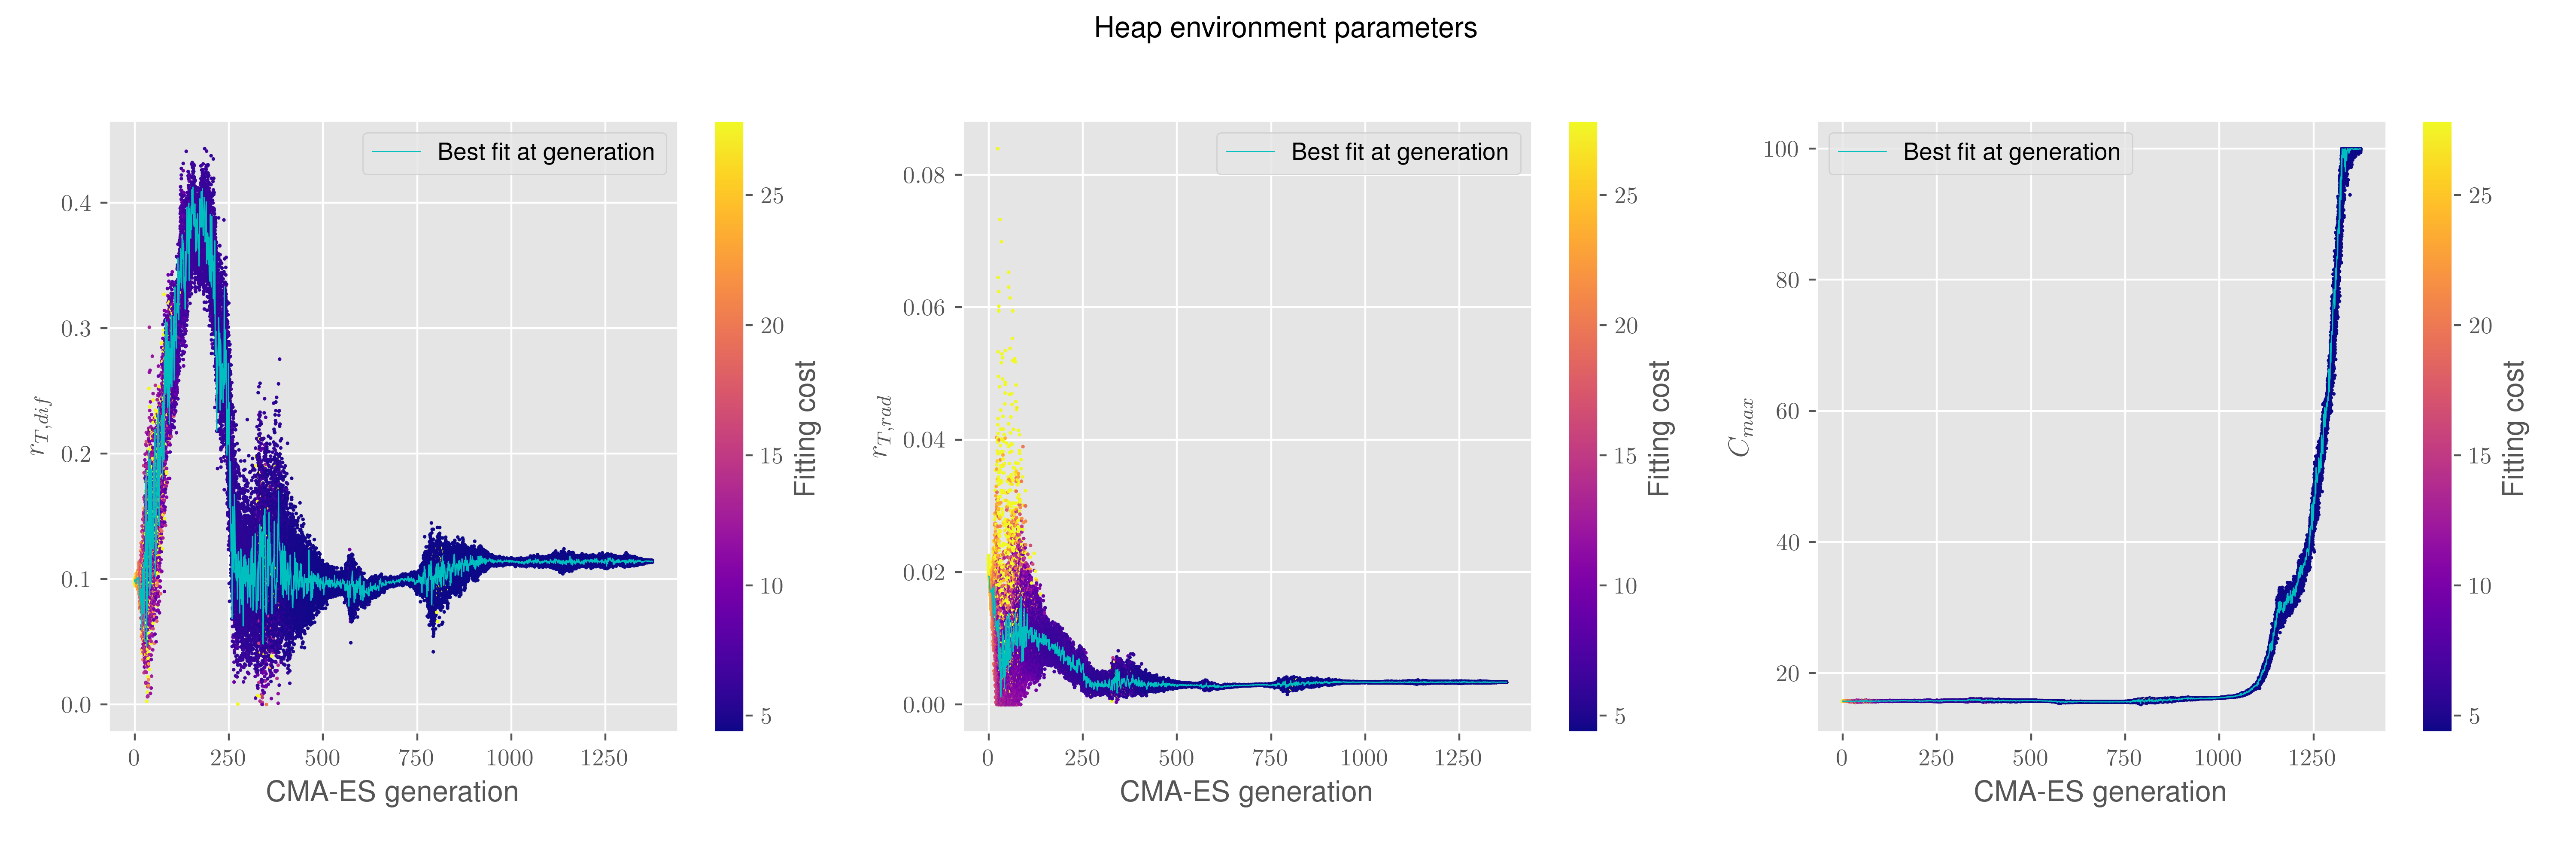
\includegraphics[width=\textwidth]{Figures/heap_parameter_evolution.png}\\
	\small Example of an algorithm working through many parameter values.
\end{frame}

\begin{frame}{Modelled temperature vs measurement}
		\centering
	\includegraphics[width=\textwidth]{Figures/GA_model_vs_all_heaps_temperature.png}
\end{frame}
\begin{frame}{Modelled 16S vs measurement}
		\centering
	\includegraphics[width=\textwidth]{Figures/GA_model_vs_all_heaps_Sensitive.png}
\end{frame}
%%%%%%%%%%%%%%%%%%%%%%%%%%%%%%%%%%%%%%%%%%%%%%%%%%%%%%%%%%%%%%%%%%%%%%%%%%%%%%%%%%%%%%%%
%\section{Experimental data informs practice}
%\subsection{Data from shed experiment}
%\begin{frame}{Resistance profiles of shed litter}
%	\centering
%	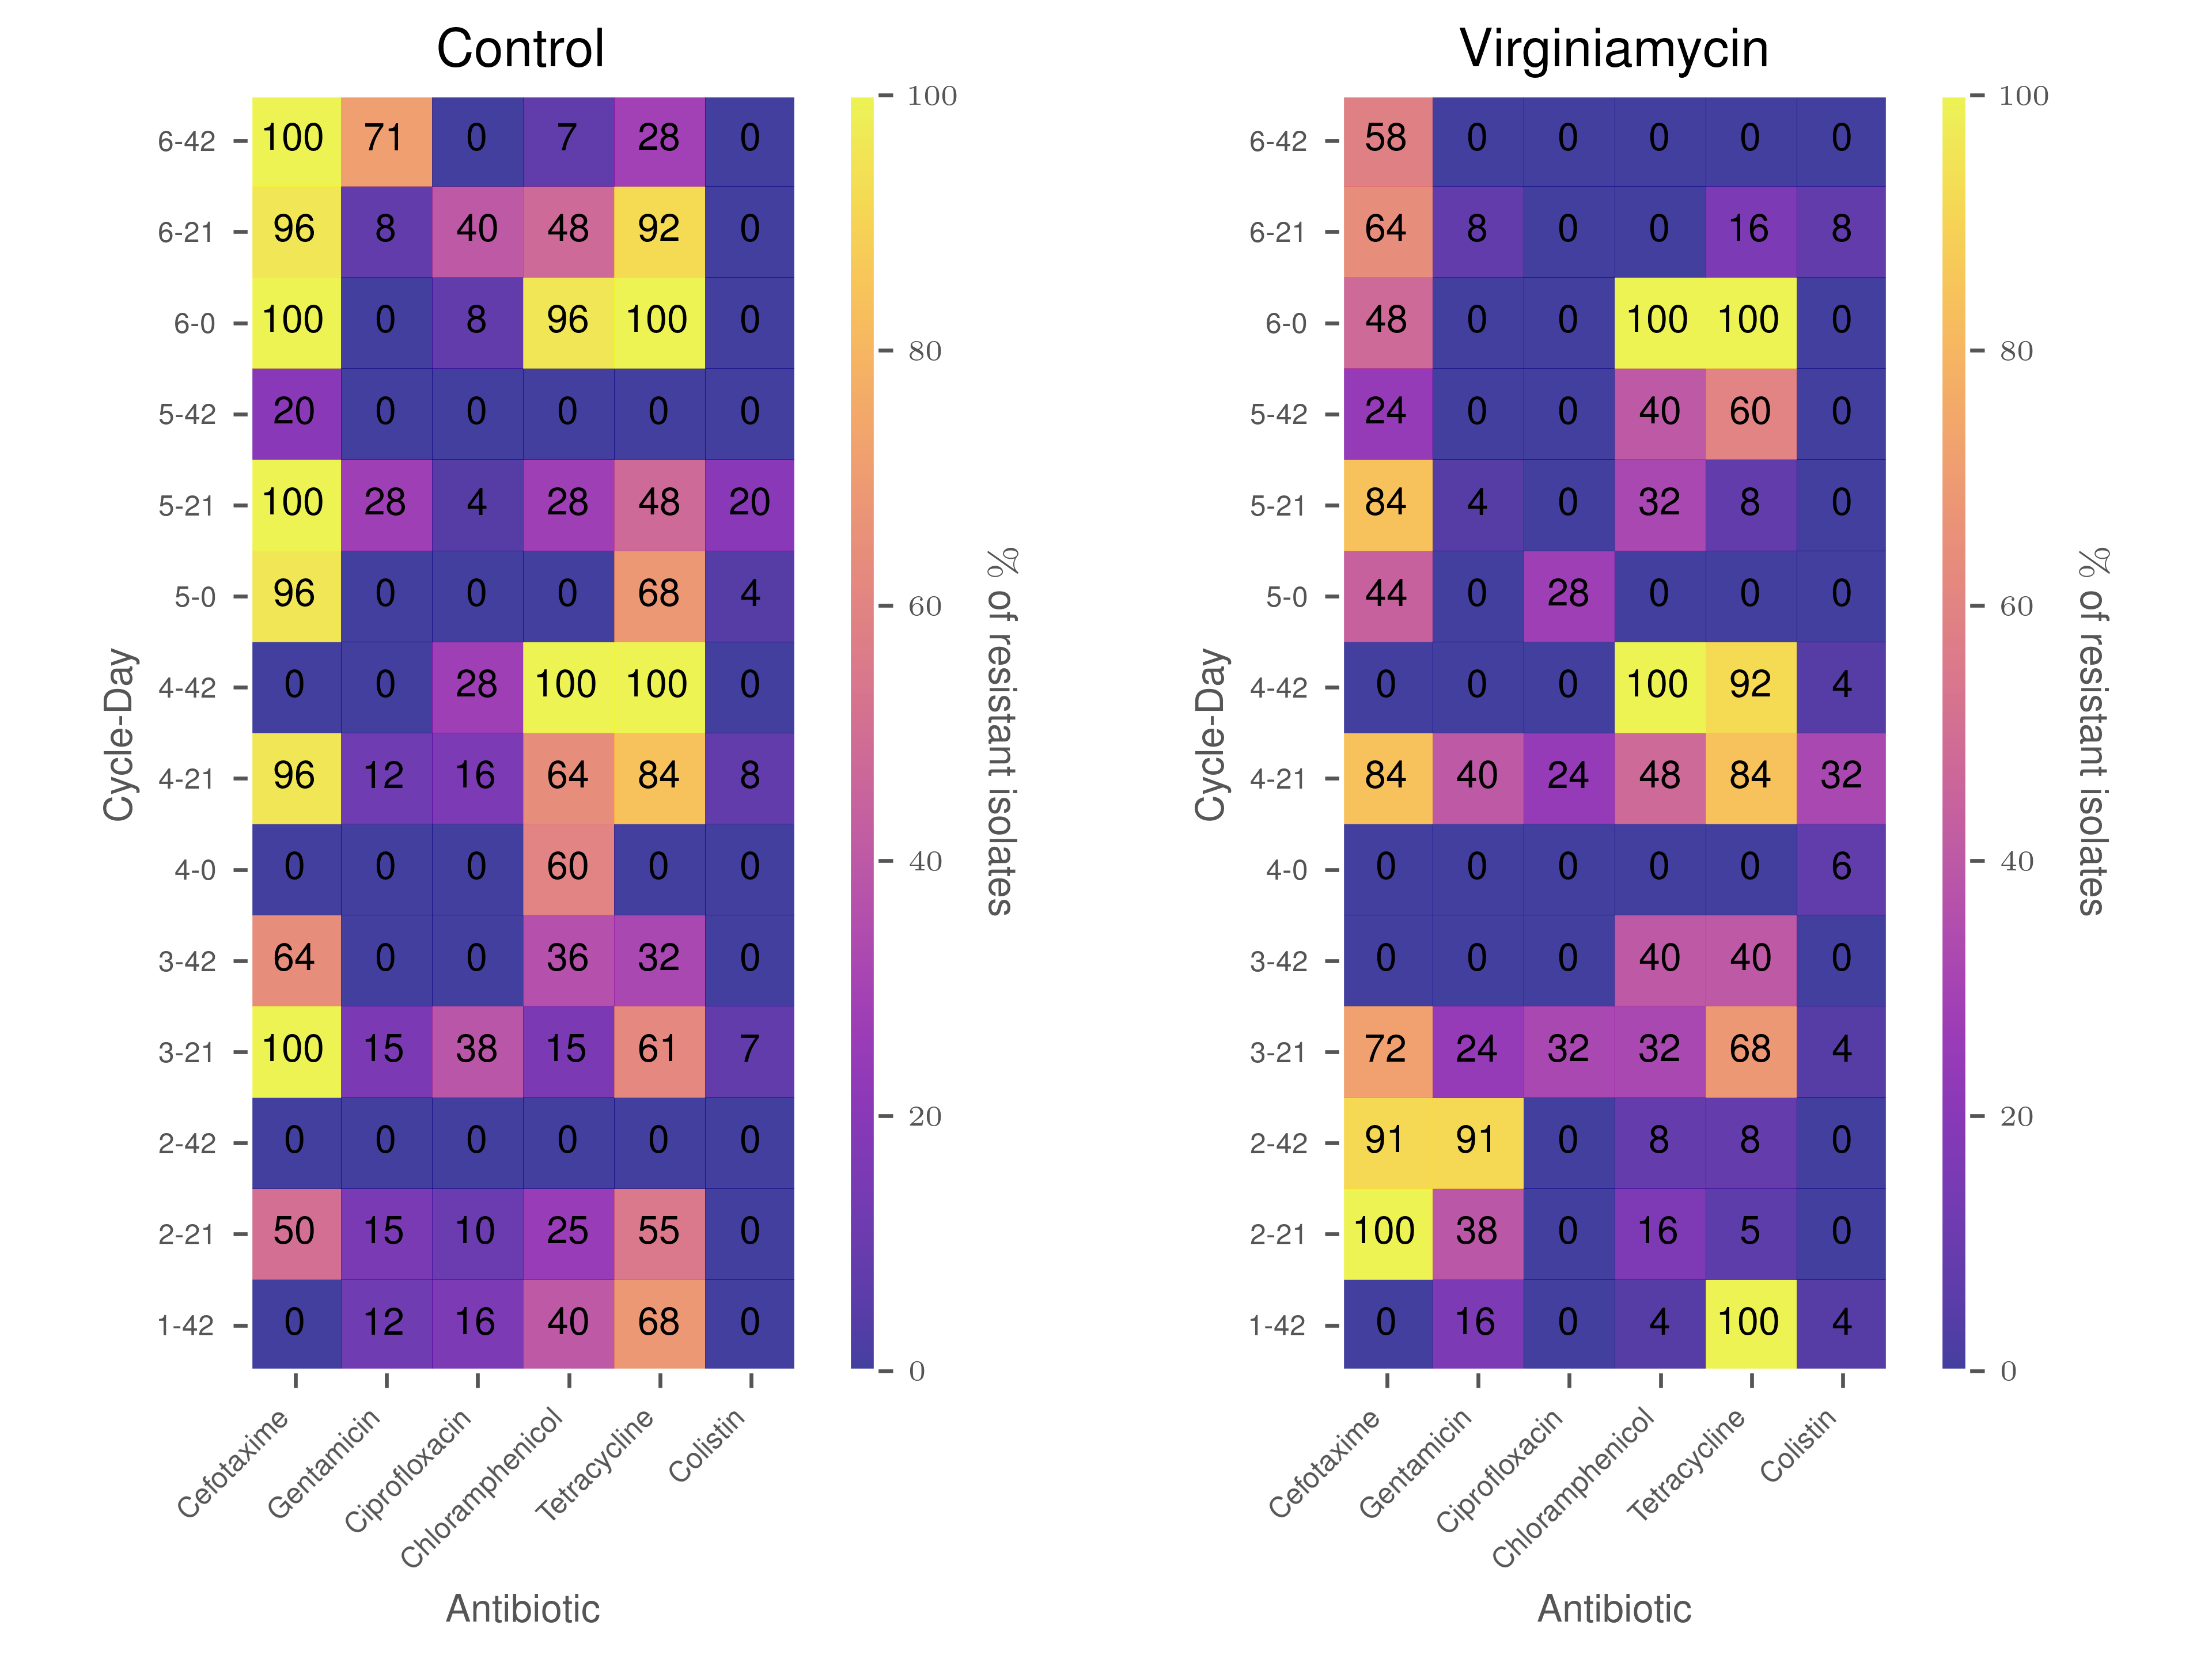
\includegraphics[width=0.8\textwidth]{Figures/Heatmaps_resistance.png}
%\end{frame}
%\subsection{Searching for patterns}
%\begin{frame}{Clustering analysis}
%	\centering
%	\includegraphics[width=0.45\textwidth]{Figures/Control_dendromap_distance.png}
%	\includegraphics[width=0.45\textwidth]{Figures/Virginiamycin_dendromap_distance.png}
%\end{frame}
%\begin{frame}{Dodgy replicates}
%	\centering
%	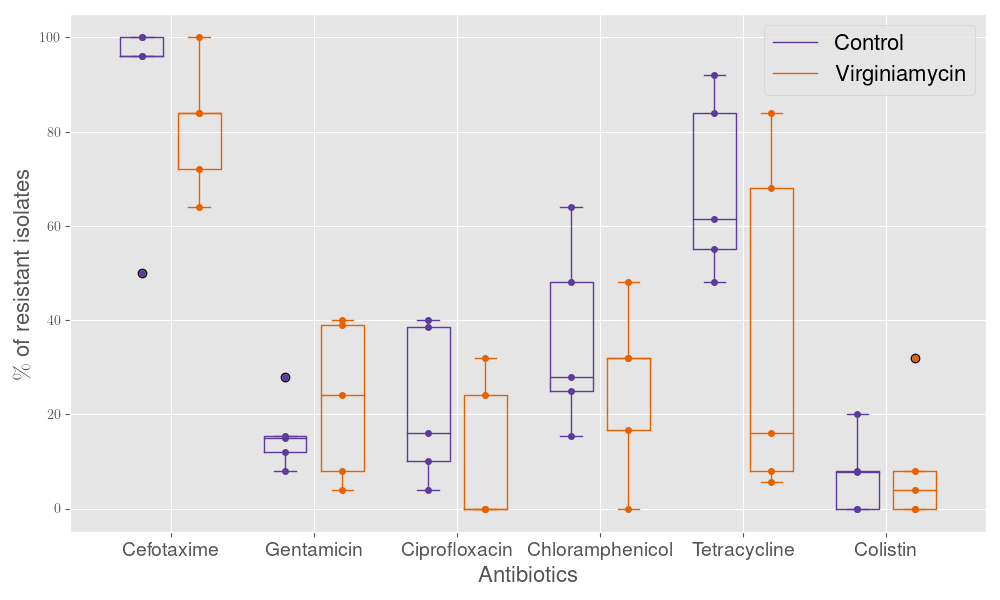
\includegraphics[width=0.8\textwidth]{Figures/Boxplots_day_21.png}\\
%	\small
%	\begin{itemize}
%		\item Used day 21 from each cycle as a replicate
%		\item Treatment effect - not significant
%		\item Drug effect - significant, requires pairwise tests.
%	\end{itemize}
%\end{frame}
%\begin{frame}{Searching for patters (contd.)}
%	\centering
%	\includegraphics<1>[width=0.8\textwidth]{Figures/Cumulative_resistance_slopes_percent.png}
%	\includegraphics<2>[width=0.8\textwidth]{Figures/Cumulative_resistance_odd_drug.png}
%	\includegraphics<3>[width=0.8\textwidth]{Figures/Cumulative_resistance_cycle_4.png}
%\end{frame}
%\begin{frame}{Productivity data}
%	\centering
%	\includegraphics<1>[width=0.8\textwidth]{Figures/Productivity.png}
%\end{frame}
%%%%%%%%%%%%%%%%%%%%%%%%%%%%%%%%%%%%%%%%%%%%%%%%%%%%%%%%%%%%%%%%%%%%%%%%%%%%%%%%%%%%%%%%
\section{Conclusion}
\begin{frame}{Is our model good?}
\vspace{0.5cm}
	\begin{itemize}
		\item<1-> \textbf{\textcolor{magenta}{Predictive power and accuracy:}} Predicts temperature changes well, but struggles with populations.
		\item<2-> \textbf{\textcolor{green}{Parsimony:}} we can simplify further and exclude pH, it does not change much.
		\item<3-> \textbf{\textcolor{magenta}{Identifiability:}} big problem with small relative abundances.
		\item<4->  \textbf{\textcolor{green}{Modular structure:}} we were able to add a measurement model to account for functional populations instead of taxonomic ones.
		\item<5-> \textbf{\textcolor{green}{Validity:}} Model outputs and measured variables can be compared directly.
	\end{itemize}
\end{frame}
\begin{frame}{Conclusion}
\begin{itemize}
	\item Association of some AMR genes and temperature tolerance observed in compost heaps: some taxa more likely to develop resistance?
	\item The temporal dynamics are more pronounces than spatial: no risk of pathogens "running to hide" in comfortable areas of the heap.
	\item Biota-driven self-heating model is able to reproduce complex temperature profiles.
	\item Identifiability issues of fitting to data from rtPCR analysis could be resolved if we knew taxa.
    \item Check how the data is distributed before running ANOVAs!
\end{itemize}	
\end{frame}
\appendix
\section<presentation>*{\appendixname}
\begin{frame}{Acknoledgements}
	\begin{columns}
			\begin{column}{0.5\textwidth}
		\small
\includegraphics[width=\textwidth,angle=270,origin=c]{Figures/heaps_helen.jpg}\\
		\small
		\textbf{Funding:}\\
		\vspace{0.2cm}
		DHSC/BBSRC\\
		CONICET
		\end{column}
		\begin{column}{0.5\textwidth}
		\footnotesize
		\textbf{UoN Biosciences, UK:}\\
			Prof Dov Stekel\\
			Dr Si\^an Powell\\
			Dr Helen West\\
		\textbf{Anlis Malbr\'an, Argentina:}\\
			Dr Sonia Gomez\\
			Bel\'en Sanz\\
		\textbf{INTA, Argentina:}\\
			Dr Leandro M Redondo\\
			Dr Mariano Fernandez Miyakawa\\
		\textbf{University of Leeds, UK:}\\
			Dr Paula Avello Fernandez\\
			Dr Graziella Iossa\\
		\textbf{CEH, UK:}\\
		Dr Andrew Singer\\
		Dr Katja Lehmann\\
		\textbf{UoN Maths Sciences, UK:}\\
		Prof Gary Mirams\\
		Dr Michael Clerx
		\end{column}
	\end{columns}
\end{frame}
\begin{frame}
\centering
\Huge{Thank you!}\\
\huge{Questions?}
\end{frame}
\end{document}